\subsubsection{Master's in Computer Science (Cybersecurity) - Portfolio Project}

\begin{framed}
\textbf{Note}\\
Minor modifications have been made to the original submitted report to correct typographical errors and for optimal presentation in Myst Markdown format.
\end{framed}

\paragraph{Download the PDF}

\href{/Mark\_Khusid\_Portfoli-d2f321973ee334c9654273bb679c38cd.pdf}{Download}

\paragraph{Portfolio Project Report: Summary}

\subparagraph{CSE548: Advanced Computer Network Security}

This summary presents the outcomes of four projects conducted within the scope of the CSE548 Advanced Network Security course, which emphasize the integration of network security principles with practical implementations and machine learning techniques. There were four individual projects in this course.

\subparagraph{Project 1: Packet Filter Firewall: Implementation of an Iptables-Based Packet Filter Firewall}

Project 1 is titled: Packet Filter Firewall: Implementation of an Iptables-Based Packet Filter Firewall.  The project involved setting up a firewall with rules ensuring controlled access and restricted communication between nodes in a simulated network.  To meet the requirements of this project, we set up an iptables firewall and a web server on a Gateway / Server virtual machine.  The iptables firewall was used to restrict network and internet access of the client as well as the  Gateway / Server as per the project requirements.  Verification of the Gateway / Server was performed and found to be in compliance.

\subparagraph{Project 2: SDN-Based Stateless Firewall: Implementation of an SDN-Based Stateless Firewall}

Project 2 is titled: SDN -- Based Stateless Firewall.  The firewall resided on an Open Virtual Switch that implements the OpenFlow protocol.  A POX instance acts as the controller for the Open Virtual Switch.  Containers are instantiated using Mininet to create four containers.  Layer 2 and Layer 3 firewall rules are applied to the controller using a firewall application running the on application plane.  Various tests are performed in order to test the functionality of the firewall application.

\subparagraph{Project 3: SDN-Based DoS Attacks and Mitigation Project}

Project 3  is titled: SDN -- Based DoS Attacks and Mitigation Project.  The purpose of this project is to learn about Software Defined Networking and implementing Denial of Service (DoS) attack mitigation.  In this project an Open Virtual Switch is created that operates on the OpenFlow protocol.  A POX instance acts as the controller for the Open Virtual Switch.  Containers are instantiated using Mininet to create four containers.  The L3 firewall application was modified to detect DoS attacks and permanently block the offending MAC address.  Various tests are performed in order to test the functionality of the firewall application.

\subparagraph{Project 4: Machine Learning-Based Anomaly Detection}

Project 4 is titled: Machine Learning -- Based Anomaly Detection.  The purpose of this Project is to use machine learning to spot abnormal patterns in network traffic and identify potential attacks from hackers.  Training data for the machine learning models is provided by the Course Team.  Two distinct models are trained and tested against three different test sets.  Testing / validation accuracy and loss are determined, as well as construction of a confusion matrix for the three separate testing conditions.  An assessment is made to determine the model with the most testing accuracy, and then to figure out why that model fares better than others.  This determination involves examining the training data and testing data to notice any particular patterns in the categories and subcategories of attacks.

\subparagraph{CSE572: Data Mining}

This summary presents the outcomes of three projects conducted within the scope of the CSE572 Data Mining course.  The first project consisted of extracting glucose level time series data and its properties for a person using an artificial pancreas.  The second project consisted of training a machine model to assess whether the person has eaten a meal or not.  The third project consisted of clustering the glucose data to determine the amount of carbohydrates the person has consumed in each meal.

\subparagraph{Project 1: Extracting Time Series Properties of Glucose Levels in Artificial Pancreas Project}

Project 1 is titled:  Extracting Time Series Properties of Glucose Levels in Artificial Pancreas Project.  Data for this project was provided as two separated Comma Separated Value (CSV) files.  The first CSV file contained CGM sensor data, while the second contained insuling pump data.  Both the CGM sensor data and insulin pump data were in reversed chronological order, meaning the latest data were the first rows of the files.  Additionally, the data from the CGM sensor and insulin pump were taken asynchronously from each other; therefore, synchronization would have to be performed.  The CGM sensor and insulin pump data also had many columns that added unecessary dimensionality that needed to be reduced.  Finally, there were many missing data points and over fifty -- five thousand rows of data.  An effective strategy was required for dealing with the missing data points and the sheer number of rows.

\subparagraph{Project 2: Machine Model Training Project}

Project 2 is titled:  Machine Model Training Project.  The goal of this project is to train a machine to differentiate between the person eating a meal versus not eating a meal given the person's CGM sensor's time series data.  As in Project 1, insulin pump and CGM sensor data were provided; however, for this project two sets of data were available.  The datasets had similar problems that occurred in Project 1; however, Project 2's insulin pump datasets had the additional issue of non -- uniform date and time recording.  This necessitated an additional step of pre -- processing of the date and time columns within the datasets.

\subparagraph{Project 3: Cluster Validation Project}

Project 3 is titled: Cluster Validation Project.  In this Project, the person's carborhydrate input provided Insulin Pump dataset is separated into bins and an unsupervised clustering algorithm is used to cluster the data and compare it to the binned ground truth.  Using techniques similar to Projects 1 and 2, the Insulin Pump data and the CGM sensor data were extracted to find the carbohydrates ingested and blood glucose levels.  As in Project 2, the CGM sensor data was cleaned, missing data imputed, features extracted and normalized.  The data were then fed into a K-Means clustering machine and a DBSCAN machine.  The results from both machines were compared and contrasted.

\paragraph{CSE548 Advanced Network Security: Portfolio Project Report}

\textbf{Abstract} --- This report presents the outcomes of four projects conducted within the scope of the CSE548 Advanced Network Security course, which emphasize the integration of network security principles with practical implementations and machine learning techniques. The projects include:

\begin{enumerate}
\item Packet Filter Firewall: Implementation of an iptables-based packet filter firewall with rules ensuring controlled access and restricted communication between nodes in a simulated network.
\item SDN-Based Stateless Firewall: Design and testing of a stateless firewall using Software Defined Networking (SDN) principles with OpenFlow and POX controller to implement Layer 2 and Layer 3 filtering.
\item SDN-Based DoS Mitigation: Identification and mitigation of Denial of Service (DoS) attacks in an SDN environment through dynamic blocking of malicious traffic using customized firewall logic.
\item Machine Learning for Anomaly Detection: Development of machine learning models to detect anomalies in network traffic using the NSL-KDD dataset, achieving significant precision and recall across multiple testing scenarios.
\end{enumerate}

The report highlights technical implementations, analytical insights, and contributions in each project.  Observations and improvements in system designs are further discussed.

\subparagraph{Introduction}

In this portfolio project report, we will be reviewing the results obtained from the four projects in this course.  The projects were:

\begin{enumerate}
\item Packet Filter Firewall (iptables) Project.
\item SDN (Software Defined Network) -- Based Stateless Firewall Project.
\item SDN (Software Defined Network) -- Based DoS (Denial of Service) Attacks and Mitigation Project.
\item Machine Learning -- Based Anomaly Detection Project.
\end{enumerate}

In Project 1 (Packet Filter Firewall (iptables), the aim was to set up and configure a packet filter firewall, test network connectivity and ensuring the proper functioning of the firewall.  In Project 2 (SDN -- Based Stateless Firewall), the aim was to delve into Software Defined Networking principles by implementing a firewall using OpenFlow \footnote{OpenFlow Switch Specification. \href{https://opennetworking.org/}{https://opennetworking.org/}} rules.  In Project 3 (SDN -- Based DoS Attacks and Mitigation Project,  the aim was to understand, detect and mitigate DoS attacks in a SDN network environment.  Finally, in Project 4 (Machine Learning -- Based Anomaly Detection), the aim was to use machine learning in identifying abnormal patterns in network traffic.  This included indications of potential threats such as intrusions or malware.

\subparagraph{Project Overviews, Setup and Descriptions}

\subparagraph{Project 1: Packet Filter Firewall (iptables) Project}

In Project 1, we set up an iptables firewall on a Gateway / Server that follows conditions determined by the following requirements:

\begin{itemize}
\item A client can send pings to 8.8.8.8 though a Gateway / Server

\begin{itemize}
\item A client can access a webpage residing on the Gateway / Server
\item A client can not access any IP addresses besides 8.8.8.8
\item The client can not ping the Gateway / Server
\item The server can not perform pings to localhost
\item The server can not perform pings to the client
\item The server can not perform pings to 8.8.8.8
\end{itemize}
\end{itemize}

The server provides Network Address Translation for the client so that packets from the client appear to come from the Gateway / Server.
A diagram of the Lab Network Topology is shown in Figure~\ref{CSE548_Fig_1}:

\begin{figure}[!htbp]
\centering
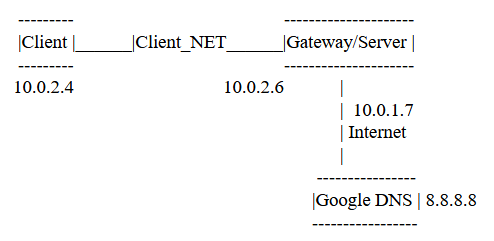
\includegraphics[width=0.7\linewidth]{files/CSE548_Fig_1-1be50f477c22b24d946ea309925d3949.png}
\caption[]{Lab Network Topology}
\label{CSE548_Fig_1}
\end{figure}

In Figure~\ref{CSE548_Fig_1} Lab Network Topology, we have a client that is connected to the 10.0.2.0 network, and a Gateway/Server that is connected to both the 10.0.2.0 and 10.0.1.0 network.  The aim is to setup a firewall and routing provisions on the Gateway/Server to satisfy the requirements mentioned above.

To setup the Project, two virtual machines were created: one for the Client, the other for the Gateway/Server.  The Client's virtual machine network setup is shown in Figure~\ref{CSE548_Fig_2}: Client Network Setup below:

\begin{figure}[!htbp]
\centering

\includegraphics[width=0.7\linewidth]{files/CSE548_Fig_2-a8a89ede2c19300be43e0ca6394f91f8.png}
\caption[]{Client Network Setup}
\label{CSE548_Fig_2}
\end{figure}

The Gateway/Server's network setup is shown in Figure~\ref{CSE548_Fig_3}: Gateway/Server Network Setup. We can see that the Gateway/Server's network setup is multi -- homed so that it can have a network port to both the 10.0.1.0 and 10.0.2.0 networks.  After the Virtual Machines were started, the Client's network setup is verified by using the ifconfig Linux command.

\begin{figure}[!htbp]
\centering
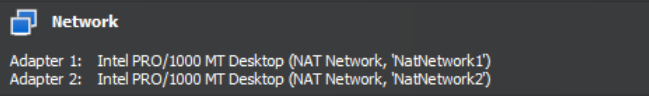
\includegraphics[width=0.7\linewidth]{files/CSE548_Fig_3-85f7088a4df2a2bf7d9fc8a3e014428e.png}
\caption[]{Gateway/Server Network Setup}
\label{CSE548_Fig_3}
\end{figure}

The output of the ifconfig Linux command is shown in Figure~\ref{CSE548_Fig_4}: Client's ifconfig Output below:

\begin{figure}[!htbp]
\centering
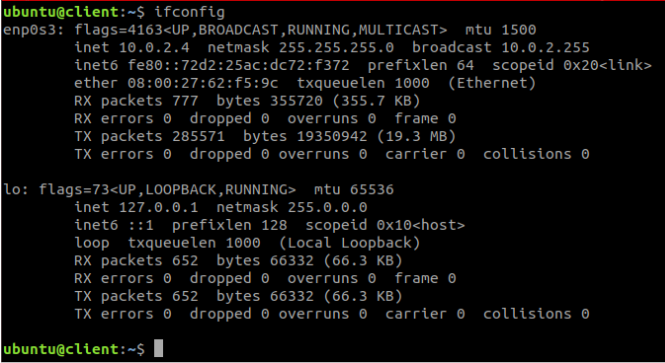
\includegraphics[width=0.7\linewidth]{files/CSE548_Fig_4-bf4bc88d89f95df222907bb0e95b02e0.png}
\caption[]{Client's \textit{ifconfig} Output}
\label{CSE548_Fig_4}
\end{figure}

As required, the Client's \textit{ifconfig} output has an IP address of 10.0.2.4.  However, for the Gateway/Server, its network port that is connected to the 10.0.2.0 network has an IP address of 10.0.2.6.  Pings from the client to the Gateway server over the 10.0.2.0 network operate as normal.  In order for the Client to be able to have access to the 10.0.1.0 network visible at the Gateway/Server's other network port, a default gateway routing entry had to be added to the Client's routing table.  This informs the the Client's operating system of how to handle packets whose IP addresses are not on the local network.  The Client's routing table is shown in Figure~\ref{CSE548_Fig_5}: Client's Routing Table below:

\begin{figure}[!htbp]
\centering
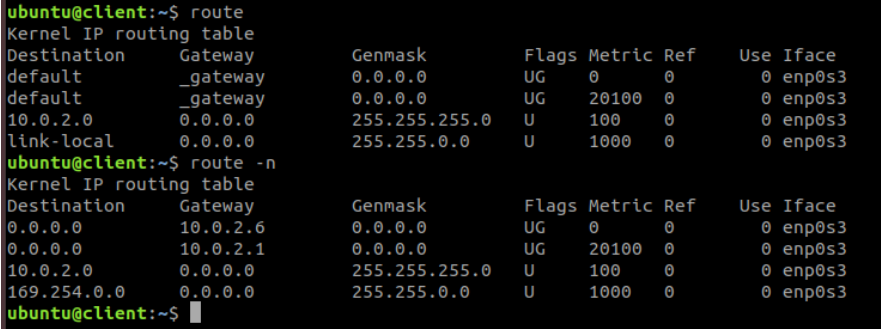
\includegraphics[width=0.7\linewidth]{files/CSE548_Fig_5-6158874c4d7b3af5609af3ee6b8fbf52.png}
\caption[]{Client's Routing Table}
\label{CSE548_Fig_5}
\end{figure}

In Figure~\ref{CSE548_Fig_5}: Client's Routing Table, we can see a entry for the default gateway whose IP address is 10.0.2.6.  The destination address for the default gateway routing table entry is 0.0.0.0, which means that any packet whose destination IP address is not on the local network (10.0.1.0) should be sent to the Gateway/Server.

The Gateway/Server was configured to be multi -- homed, with two network interfaces.  The output of the ifconfig Linux command when executed on the Gateway/Server is shown in Figure~\ref{CSE548_Fig_6}: Gateway/Server's ifconfig Output.

\begin{figure}[!htbp]
\centering
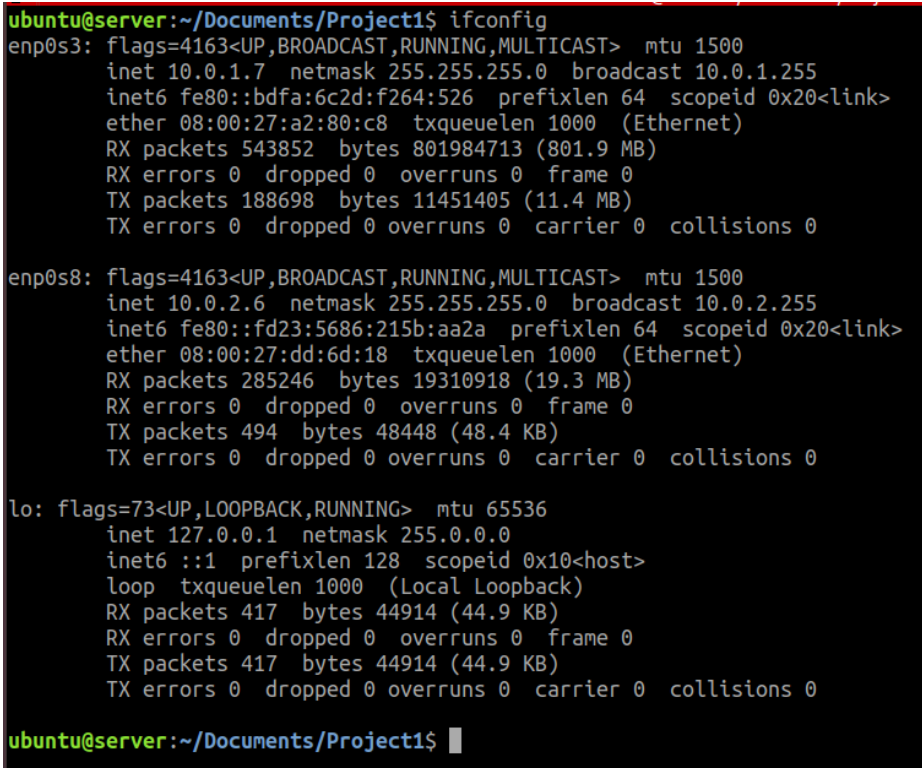
\includegraphics[width=0.7\linewidth]{files/CSE548_Fig_6-ee31ad79008ada53252c0d20c55a6570.png}
\caption[]{Gateway/Server's \textit{ifconfig} Output}
\label{CSE548_Fig_6}
\end{figure}

As can be seen in Figure~\ref{CSE548_Fig_6}: Gateway/Server's ifconfig Output, the Gateway/Server is connected to both the 10.0.1.0 and 10.0.2.0 networks.
In order for the Gateway/Server to allow pings to the IP address 8.8.8.8, Network Address Translation (NAT) was implemented as shown in Figure~\ref{CSE548_Fig_7}: Gateway/Server's NAT Setup below:

\begin{figure}[!htbp]
\centering
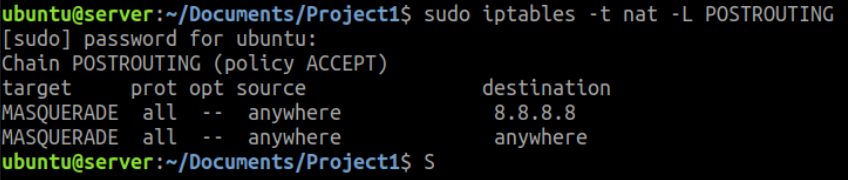
\includegraphics[width=0.7\linewidth]{files/CSE548_Fig_7-1d5e0af006016290c95e16d83ad421e4.png}
\caption[]{Gateway/Server's NAT Setup}
\label{CSE548_Fig_7}
\end{figure}

In Figure~\ref{CSE548_Fig_7}: Gateway/Server's NAT Setup, a Masquerade entry was added that allowed for network address translation for the reply pings coming back from the pinged IP address 8.8.8.8).  If this entry didn't exist, then reply pings would never be received by the Client.
A simple web server was implemented on the Gateway/Server.  The web content for the server was the message ``Welcome to Demo and Test!''.  This content was stored in an html file as shown in Figure~\ref{CSE548_Fig_8}: Gateway/Server's Web Content below:

\begin{figure}[!htbp]
\centering
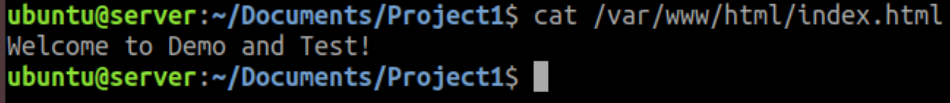
\includegraphics[width=0.7\linewidth]{files/CSE548_Fig_8-6e9a8a87053d5a00a601aeb88f92f5b0.png}
\caption[]{Gateway/Server's Web Content}
\label{CSE548_Fig_8}
\end{figure}

An Apache \footnote{Apache HTTP Server. \href{https://httpd.apache.org/}{https://httpd.apache.org/}} webserver was started Gateway/Server.  The status of the webserver is shown in Figure~\ref{CSE548_Fig_9}: Apache Webserver's Status below:

\begin{figure}[!htbp]
\centering
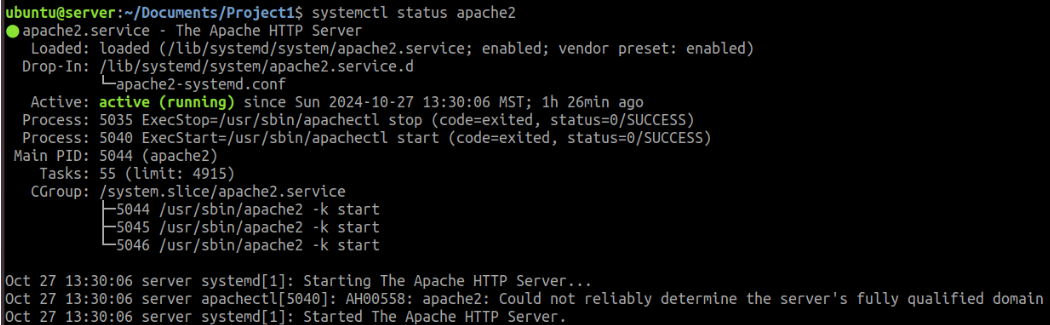
\includegraphics[width=0.7\linewidth]{files/CSE548_Fig_9-9013544693c5b01520ffba63d0d69850.png}
\caption[]{Apache Webserver's Status}
\label{CSE548_Fig_9}
\end{figure}

\subparagraph{Project 2: SDN-Based Stateless Firewall}

In Project 2, we setup a Software Defined Networking Stateless Firewall.  The firewall resided on an Open Virtual Switch that implements the OpenFlow protocol.  A POX \footnote{Using the POX SDN Controller. \href{https://brianlinkletter.com/2015/04/using-the-pox-sdn-controller/}{https://brianlinkletter.com/2015/04/using-the-pox-sdn-controller/}}  instance acts as the controller for the Open Virtual Switch.  Containers are instantiated using Mininet to create four containers.  Layer 2 and Layer 3 firewall rules are applied to the controller using a firewall application running the application plane.  Various tests are performed in order to test the functionality of the firewall application.

The network setup for this Project is shown in Figure~\ref{CSE548_Fig_10}: Project 2 Network Setup below:

\begin{figure}[!htbp]
\centering
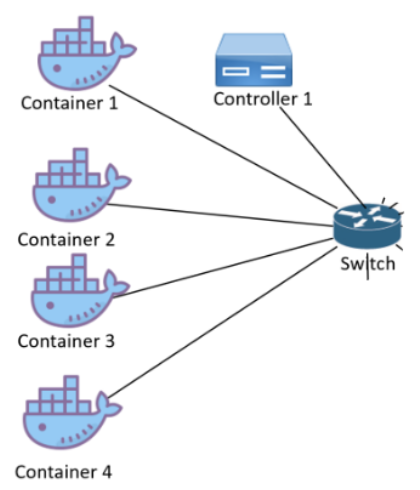
\includegraphics[width=0.7\linewidth]{files/CSE548_Fig_10-0c62471eea2bbedc2c1614ff8e71d72b.png}
\caption[]{Project 2 Network Setup}
\label{CSE548_Fig_10}
\end{figure}

Figure~\ref{CSE548_Fig_10}: Project 2 Network Setup shows the network topology.  The default IP addresses were changed such that the containers have the following IP addresses:

\begin{itemize}
\item Container 1: 192.168.2.10
\item Container 2: 192.168.2.20
\item Container 3: 192.168.2.30
\item Container 4: 192.168.2.40
\end{itemize}

The default firewall rules did not prevent reachability between the containers.  Firewall rules were added per the Project instructions and tests were performed to check the functionality of the firewall with the new rules.

To setup the controller, the following POX command was issued as shown in Figure~\ref{CSE548_Fig_11}: POX Instantiation Command:

\begin{figure}[!htbp]
\centering
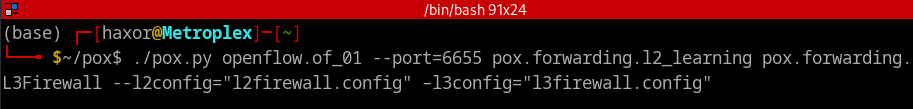
\includegraphics[width=0.7\linewidth]{files/CSE548_Fig_11-9ced168e2dcf5acb9ae43ac69e64ace1.png}
\caption[]{POX Instantiation Command}
\label{CSE548_Fig_11}
\end{figure}

The POX instantiation command shown in Figure~\ref{CSE548_Fig_11}: POX Instantiation Command starts a POX controller using the OpenFlow protocol, using port 6655, with a Layer 2 learning firewall and a Layer 3 forwarding firewall.

To setup the Containers (Clients), the following Mininet \footnote{Mininet: An Instant Virtual Network on your Laptop (or other PC). \url{http://mininet.org/}} command was issued as shown in Figure~\ref{CSE548_Fig_12}: Host Network Configurations below:

\begin{figure}[!htbp]
\centering
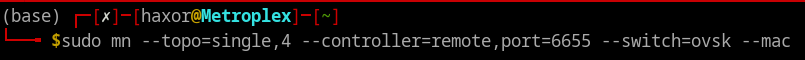
\includegraphics[width=0.7\linewidth]{files/CSE548_Fig_12-b5ebd6e5d0b9c1486715b1debfea6dc8.png}
\caption[]{Host Network Configurations}
\label{CSE548_Fig_12}
\end{figure}

Issuing the command shown in Figure~\ref{CSE548_Fig_12}: Mininet Instantiation Command created four containers that attached themselves to the Open Virtual Switch listening on port 6655, with MAC (Media Access Control) functionality enabled.  The output of the command is shown in Figure~\ref{CSE548_Fig_13}: Output of Mininet Command below:

\begin{figure}[!htbp]
\centering
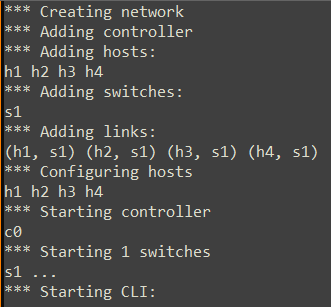
\includegraphics[width=0.7\linewidth]{files/CSE548_Fig_13-0467043b2f4ccf8077df05415b1a7f8f.png}
\caption[]{Output of Mininet Command}
\label{CSE548_Fig_13}
\end{figure}

In the Mininet output shown in Figure~\ref{CSE548_Fig_13}: Output of Mininet Command, we can see that 4 hosts are created, and attached to switch s1.  Links were added between the hosts and s1.  Once the links were established, the hosts were configured with IP addresses and the Controller and Switch were started.

The default IP addesses given to the hosts were not in compliance with the Project requirements; therefore, their IP addresses were changed using the Linux \textit{ifconfig} command.  The results of the issued \textit{ifconfig} commands for each host are shown in the following figures (Figure~\ref{CSE548_Fig_14a}, Figure~\ref{CSE548_Fig_14b}, Figure~\ref{CSE548_Fig_14c}, Figure~\ref{CSE548_Fig_14d}) below:

\begin{figure}[!htbp]
\centering
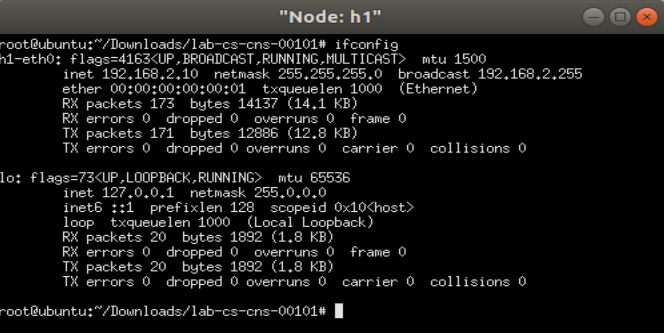
\includegraphics[width=0.7\linewidth]{files/CSE548_Fig_14a-bf21651112156987f282403ef982994a.png}
\caption[]{Host 1's \textit{ifconfig} Output}
\label{CSE548_Fig_14a}
\end{figure}

\begin{figure}[!htbp]
\centering
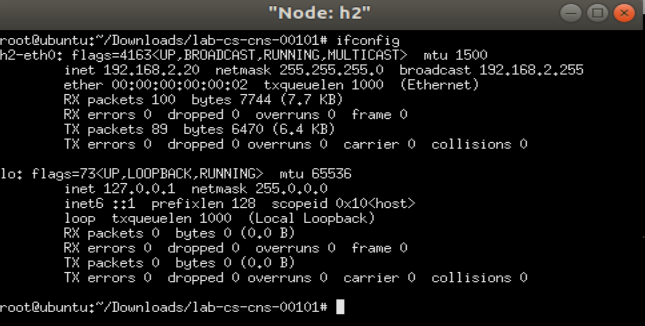
\includegraphics[width=0.7\linewidth]{files/CSE548_Fig_14b-caaa6e52179e5fdc0b1d51f75d112ab0.png}
\caption[]{Host 2's \textit{ifconfig} Output}
\label{CSE548_Fig_14b}
\end{figure}

\begin{figure}[!htbp]
\centering
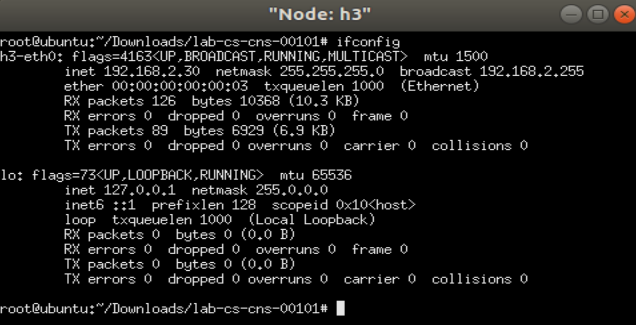
\includegraphics[width=0.7\linewidth]{files/CSE548_Fig_14c-cff910f28ebc3438452d3b911f9b9102.png}
\caption[]{Host 3's \textit{ifconfig} Output}
\label{CSE548_Fig_14c}
\end{figure}

\begin{figure}[!htbp]
\centering
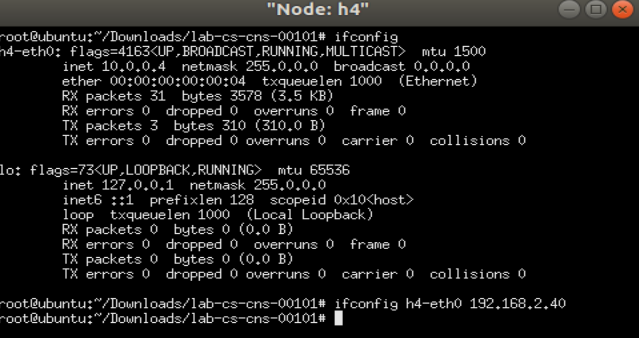
\includegraphics[width=0.7\linewidth]{files/CSE548_Fig_14d-41f13cd84bc136a42ae2c89e97af849b.png}
\caption[]{Host 4's \textit{ifconfig} Output}
\label{CSE548_Fig_14d}
\end{figure}

As can be seen in Figure~\ref{CSE548_Fig_14a}, Figure~\ref{CSE548_Fig_14b}, Figure~\ref{CSE548_Fig_14c}, Figure~\ref{CSE548_Fig_14d}: Host Network Configurations, every host's IP address was changed from the default 10.0.0.0 network to the 192.168.2.0 network.

\subparagraph{Project 3: SDN-Based DoS Attacks and Mitigation Project}

The purpose of this project is to learn about Software Defined Networking and implementing Denial of Service (DoS) attack mitigation.  In this project an Open Virtual Switch is created that operates on the OpenFlow protocol.  A POX instance acts as the controller for the Open Virtual Switch.  Containers are instantiated using Mininet to create four containers.  The L3 firewall application was modified to detect DoS attacks and permanently block the offending MAC address.  Various tests are performed in order to test the functionality of the firewall application.
Setup for this Project is the same as for Project 2, except that the POX controller was now started with a Layer 3 learning firewall.  The initiation command for the POX controller is shown in Figure~\ref{CSE548_Fig_18}: Starting Layer 3 Learning Application through POX below:

\begin{figure}[!htbp]
\centering
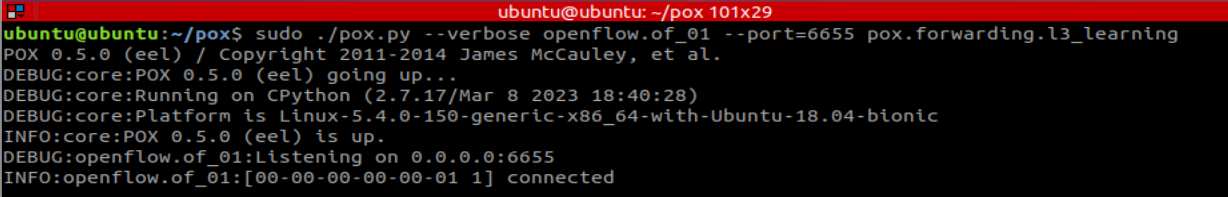
\includegraphics[width=0.7\linewidth]{files/CSE548_Fig_18-27c7e1d6f87fa5d0ba70424e62969a08.png}
\caption[]{Starting Layer 3 Learning Application through POX}
\label{CSE548_Fig_18}
\end{figure}

The Layer 3 Learning application started using the command shown in Fig 15: Starting Layer 3 Learning Application through POX, instantiates a Open Virtual Switch whose Layer 3 firewall is defined in the pox.forwarding.l3\_learning configuration file.  The Layer 3 configuration is defined in a Python script attached to this document \href{/sections/mcs-projects/mcs-portfolio-project/l3firewall}{L3Firewall.py}

\subparagraph{Project 4: Machine Learning-Based Anomaly Detection}

The purpose of this Project is to use machine learning to spot abnormal patterns in network traffic and identify potential attacks from hackers.  Training data for the machine learning models is provided by the Course Team.  Two distinct models are trained and tested against three different test sets.  Testing / validation accuracy and loss are determined, as well as construction of a confusion matrix for the three separate testing conditions.  An assessment is made to determine the model with the most testing accuracy, and then to figure out why that model fares better than others.  This determination involves examining the training data and testing data to notice any particular patterns in the categories and subcategories of attacks.

The analysis was performed in a Virtualbox Linux virtual machine (VM) guest running on a Windows 11 host.  The Linux system is Parrot OS.  The VM was assigned 12/16 processors and 24 Gbytes of RAM.  Unfortunately, Virtualbox does not support GPU passthrough to the guest and using the GPU for model training was not possible.  Model training was performed on the CPU with an average training time of about 2.5 hours per scenario.
The course team provided the bare-bones Python code necessary to make inroads into the Project.  Specifically, a data extractor script was provided to extract specific classes of attacks from the NSL-KDD standard cybersecurity dataset.  The data extractor script was migrated into a Jupyter Lab notebook running a Python 3.11 kernel.  The notebook is provided as an attachment to this Report \href{/sections/mcs-projects/mcs-portfolio-project/dataextractor}{Data Extractor}.  Migrating the data extractor script into Jupyter Lab provided a means of monitoring the operation of the script in logical sections.  The data extractor script was used to create training and testing data per the Project specifications.

After the training and testing datasets were extracted, the next script that was provided by the Course Team and migrated into Jupyter Lab was FNN\_sample.py.  This script contained the bulk of the work necessary to be completed for the Project.  The script was modified to use the training and testing datasets per the Project specifications.  To facilitate reuse, a separate Jupyter Lab notebook file was create for each of the three scenarios.  These notebooks are provided as an attachment to this report \href{/sections/mcs-projects/mcs-portfolio-project/fnn-sample-sa}{FNN Sample SA}, \href{/sections/mcs-projects/mcs-portfolio-project/fnn-sample-sb}{FNN Sample SB}, \href{/sections/mcs-projects/mcs-portfolio-project/fnn-sample-sc}{FNN Sample SC}.

The Python Modules Keras \footnote{Keras. \url{https://keras.io/}} and Tensorflow \footnote{TensorFlow. \href{https://www.tensorflow.org/}{https://www.tensorflow.org/}} were the backends that provided the framework for training and testing the Feedforward Neural Networks.

The first step was to obtain the NSL-KDD \footnote{NSL-KDD Dataset. \href{https://www.unb.ca/cic/datasets/nsl.html}{https://www.unb.ca/cic/datasets/nsl.html}} dataset per the Project instructions.  The dataset was obtained and examined within Jupyter Lab.  The first few lines of the dataset are shown in Figure~\ref{CSE548_Fig_19}: NSL-KDD Dataset Excerpt below:

\begin{figure}[!htbp]
\centering
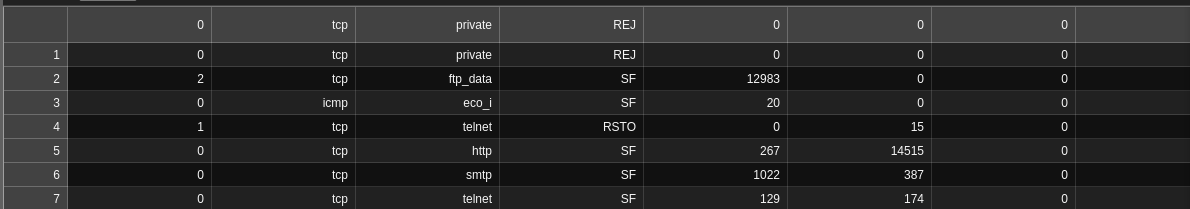
\includegraphics[width=0.7\linewidth]{files/CSE548_Fig_19-38b104783df56addb007b9343b4f172a.png}
\caption[]{NSL-KDD Dataset Excerpt}
\label{CSE548_Fig_19}
\end{figure}

Figure~\ref{CSE548_Fig_19}: NSL-KDD Dataset Excerpt shows that the data is a CSV file with many rows and columns (only a few rows and columns are visible above).  A description is provided in an attached HTML file.  Task 2 of the Project instructions called out using the KDDTrain+.txt and KDDTest+.txt files, and obtaining attack classes and subclasses from them.  The KDDTrain+.csv and KDDTest+.txt raw data is opened in Jupyter Lab and shown in Figure~\ref{CSE548_Fig_20}: KDDTrain+.txt (partial) and Figure~\ref{CSE548_Fig_21}: KDDTest+.txt (partial) below:

\begin{figure}[!htbp]
\centering
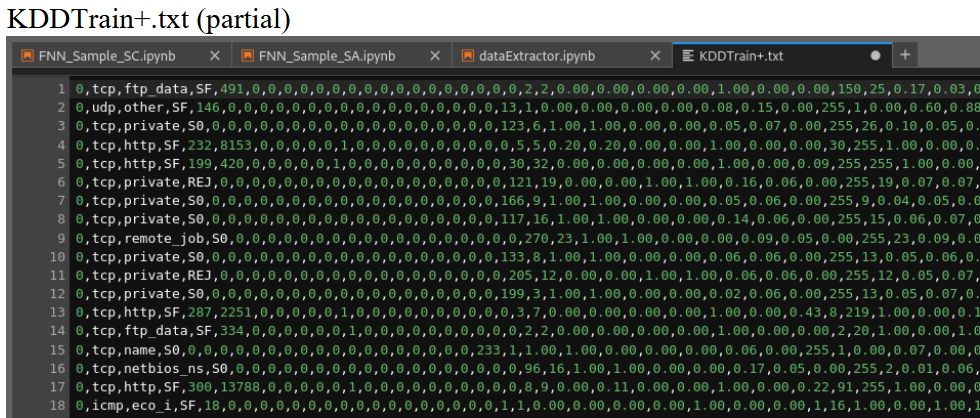
\includegraphics[width=0.7\linewidth]{files/CSE548_Fig_20-013795b4b6531974f2d78352a0712463.png}
\caption[]{KDDTrain+.txt (partial)}
\label{CSE548_Fig_20}
\end{figure}

\begin{figure}[!htbp]
\centering
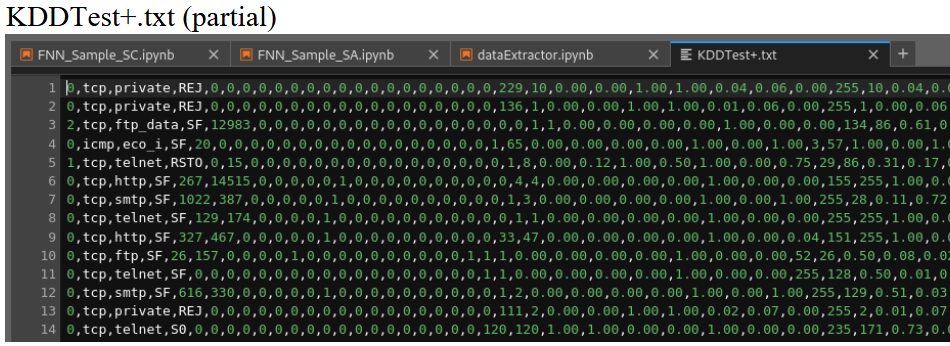
\includegraphics[width=0.7\linewidth]{files/CSE548_Fig_21-8ae502528d93b305f92df1bedc26caf2.png}
\caption[]{KDDTest+.txt (partial)}
\label{CSE548_Fig_21}
\end{figure}

In Figure~\ref{CSE548_Fig_20}: KDDTrain+.txt (partial) and Figure~\ref{CSE548_Fig_21}: KDDTest+.txt (partial), we can see that the files contain large amounts of categorical and numerical data.  The class labels are at the second to last column (not shown for brevity).  	As denoted by their filenames, the data in KDDTrain+.txt will be used to train the machine learning model, and KDDTest+.txt will be used for testing the machine learning models.

Task 2 of the Project calls out the following scenarios shown in Table~\ref{CSE548_Table_1}: Train / Test Scenarios:

\begin{table}
\centering
\caption[]{Train / Test Scenarios}
\label{CSE548_Table_1}
\begin{tabular}{p{\dimexpr 0.250\linewidth-2\tabcolsep}p{\dimexpr 0.250\linewidth-2\tabcolsep}p{\dimexpr 0.250\linewidth-2\tabcolsep}p{\dimexpr 0.250\linewidth-2\tabcolsep}}
\toprule
Datasets & Scenario A (SA) & Scenario B (SB) & Scenario C (SC) \\
\hline
Training Dataset & A1, A3, N & A1, A2, N & A1, A2, N \\
Testing Dataset & A2, A4, N & A1, N & A1, A2, A3, N \\
\bottomrule
\end{tabular}
\end{table}

We can see that there are three scenarios with different testing requirements, although scenario B and scenario C share a common training dataset.  This commonality greatly reduces the amount of model training time.

For Scenario A, the distribution of attack types is shown in Figure~\ref{CSE548_Fig_22}: A1 and A3 Training Dataset Distribution of Attack Types below:

\begin{figure}[!htbp]
\centering
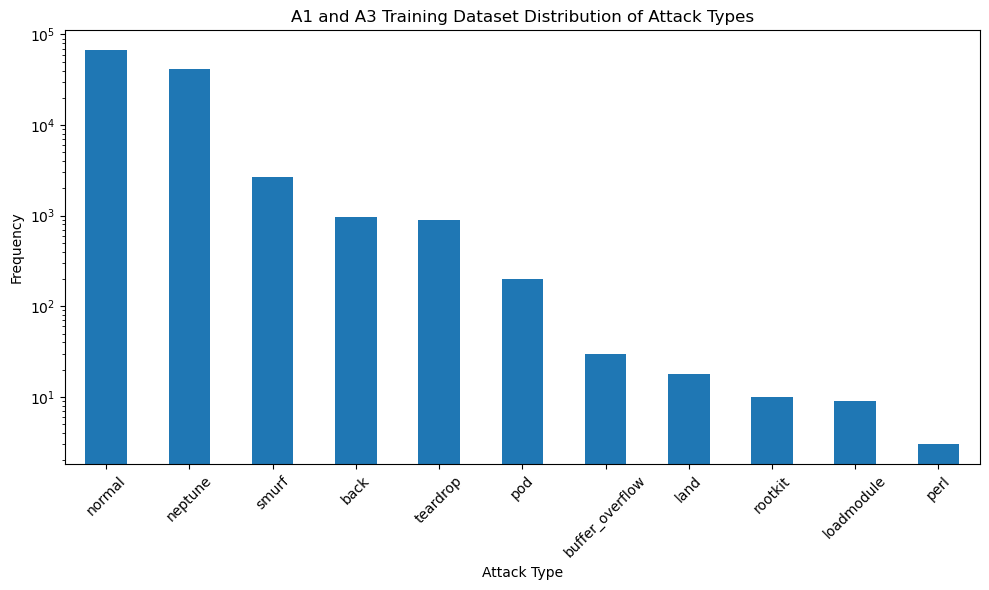
\includegraphics[width=0.7\linewidth]{files/CSE548_Fig_22-0da7daa8ffff28a6a08389c81668a56f.png}
\caption[]{A1 and A3 Training Dataset Distribution of Attack Types}
\label{CSE548_Fig_22}
\end{figure}

Scenario B and C had the following attack distribution shown in Figure~\ref{CSE548_Fig_23}: A1 and A2 Training Dataset Distribution of Attack Types below:

\begin{figure}[!htbp]
\centering
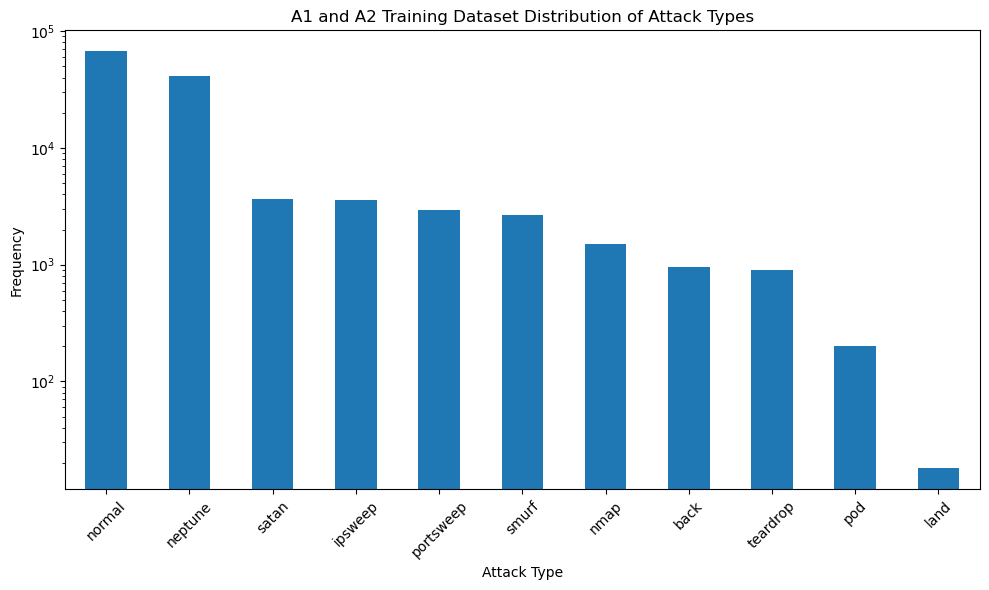
\includegraphics[width=0.7\linewidth]{files/CSE548_Fig_23-5822ac6a419b28936e0c5744977e6c4a.png}
\caption[]{A1 and A2 Training Dataset Distribution of Attack Types}
\label{CSE548_Fig_23}
\end{figure}

Of particular interest is how the trained models would perfom when tested on data that is not included in their training data.  To that end, the test data for Scenario A is shown in Figure~\ref{CSE548_Fig_24}: A2 and A4 Testing Dataset Distribution of Attack Types.

\begin{figure}[!htbp]
\centering
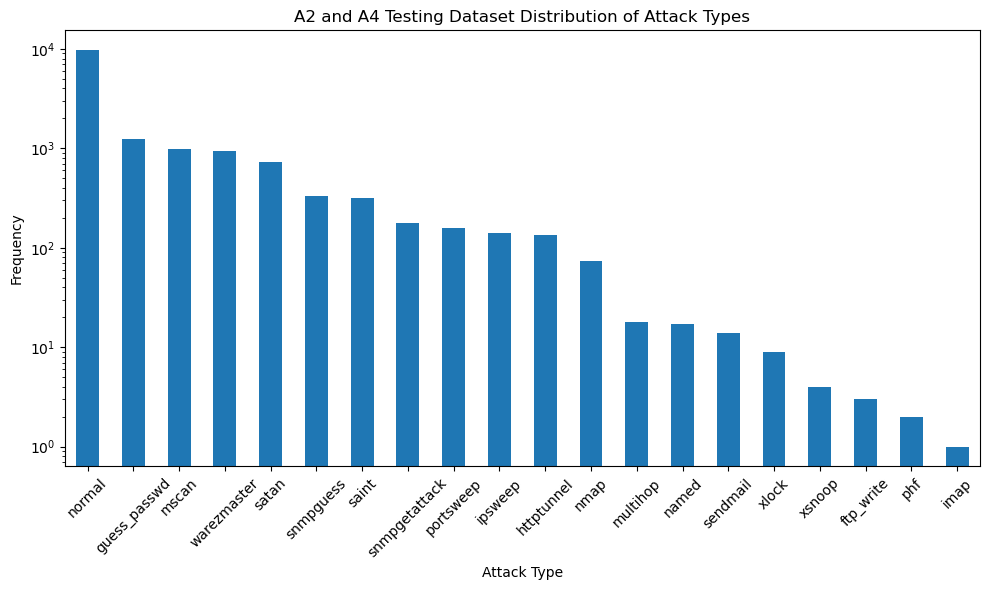
\includegraphics[width=0.7\linewidth]{files/CSE548_Fig_24-e601d85111ea97a754027d75cd973e16.png}
\caption[]{A2 and A4 Testing Dataset Distribution of Attack Types}
\label{CSE548_Fig_24}
\end{figure}

We can see that in Scenario A, the model is trained on subclasses A1 and A3 but tested on A2 and A4.  A similar situtation was applied for Scenario B and C.

A distribution of the attacks in the testing data for Scenario B is shown in Figure~\ref{CSE548_Fig_25}: A1 Testing Dataset Distribution of Attack Types.

\begin{figure}[!htbp]
\centering
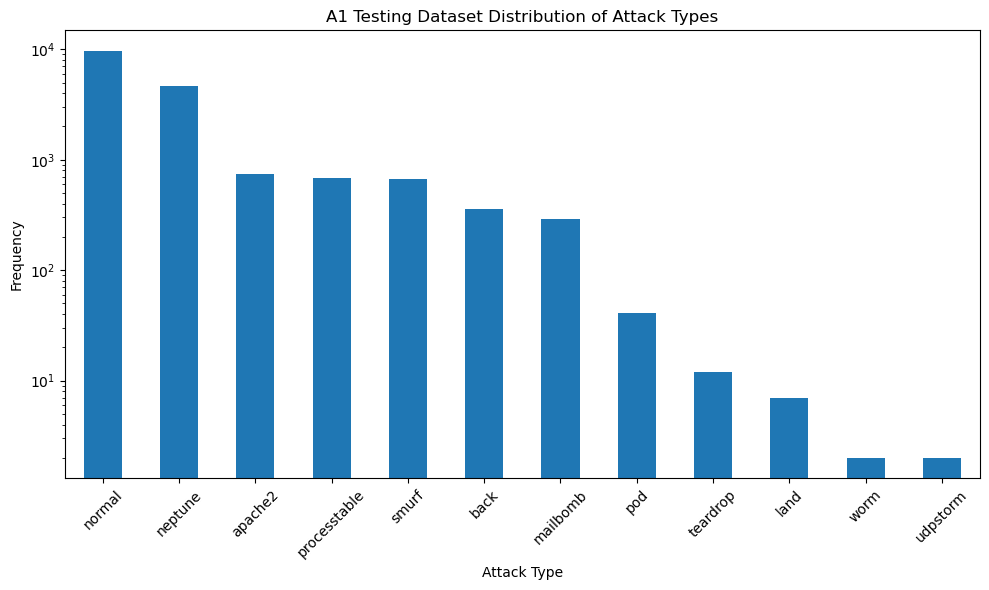
\includegraphics[width=0.7\linewidth]{files/CSE548_Fig_25-65ddebf61e0773752e9e9966728c4ec3.png}
\caption[]{A1 Testing Dataset Distribution of Attack Types}
\label{CSE548_Fig_25}
\end{figure}

Similarly, the testing data for Scenario C is shown in Figure~\ref{CSE548_Fig_26}: A1, A2 and A3 Testing Dataset Distribution of Attack Types.

\begin{figure}[!htbp]
\centering
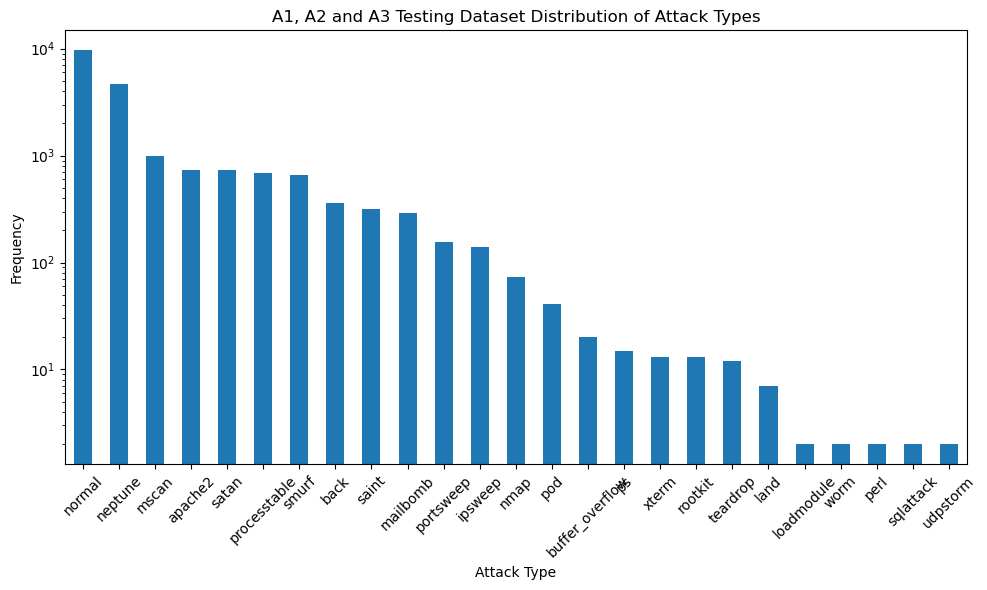
\includegraphics[width=0.7\linewidth]{files/CSE548_Fig_26-15a5431ce8754c4b364cf3c99bfb9b3f.png}
\caption[]{A1, A2 and A3 Testing Dataset Distribution of Attack Types}
\label{CSE548_Fig_26}
\end{figure}

\subparagraph{Data Preparation: One - Hot Encoding}

Since we will be training a neural network, all string objects in the dataset need to be processed into numeric values.  A convenient method is ``one -- hot encoding'', where each category gets its own column and a ``1'' for that particular category in the data row.  The categorical data was converted into numerical data by using One -- Hot Encoding from the SKLearn \footnote{Scikit-learn. \href{https://scikit-learn.org/}{https://scikit-learn.org/}} Python library.

\subparagraph{Data Preparation: Feature Scaling}

To improve accuracy of the neural network, it is important that features with large ranges do not swamp out the features with smaller ranges.  For this reason, all of the numerical data is normalized using SKLearn's Standard Scaler.

\subparagraph{Model Training}

The models were then trained on the conditioned data.  These tasks are performed in the FNN\_Sample\_SX Jupyter Notebooks (where X is either A, B or C.  See attached Jupyter Notebooks).  Training a FNN is a very time consuming process; therefore, once trained, the network weights and biases were saved into a Keras format for later recall.  When saving the models training weights and biases, the loss history is not saved.  It was therefore recorded into JSON files for later recall.

The models were then reloaded into memory and a summary was viewed.  Keras provides a method to observe a summary of the trained model.  The summary for Scenario A is shown in Figure~\ref{CSE548_Fig_27}: Scenario A Trained Model Summary below:

\begin{figure}[!htbp]
\centering
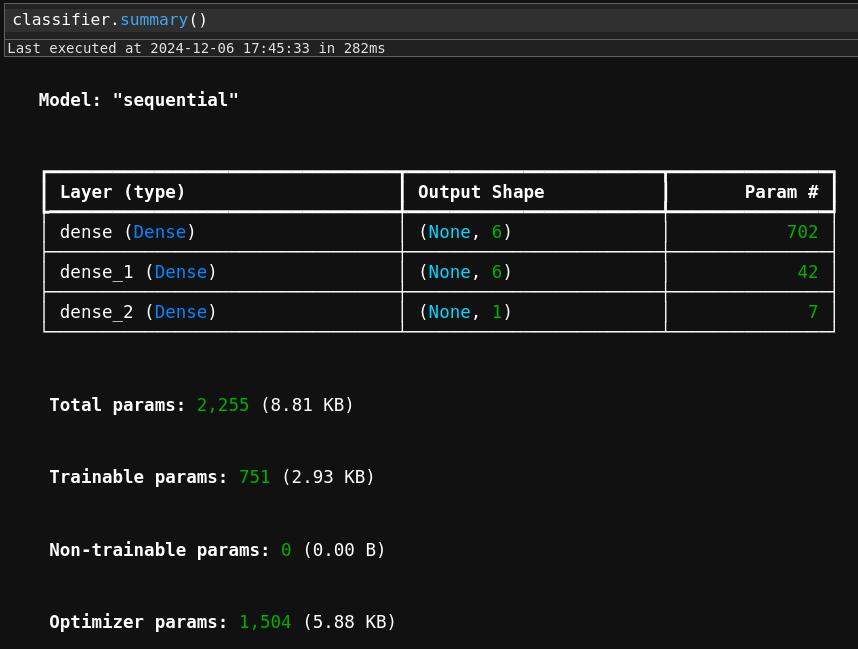
\includegraphics[width=0.7\linewidth]{files/CSE548_Fig_27-864215c9d5998cfe08cc827f13156c63.png}
\caption[]{Scenario A Trained Model Summary}
\label{CSE548_Fig_27}
\end{figure}

Per Figure~\ref{CSE548_Fig_27}: Scenario A Trained Model Summary, the structure of the neural network is a dense layer of 6 input neurons, 6 inner neurons and one output neuron.  The output neuron outputted a value between 0 and 1, where a value greater than 0.9 was considered as an attack, and normal otherwise.  The number of epochs was 10 and the batch size was selected to be 10.  These values seemed to provide good (i.e.\textgreater  0.95) training accuracy and low (\textless 0.1) loss for this particular neural network architecture and datasets.  Similar summaries are obtained for Scenario's B and C.

\subparagraph{Explanation of Solution}

\subparagraph{Project 1: Packet Filter Firewall (iptables) Project}

In order to meet the requirements of the Project, \texttt{iptables} rules were created such that network actions comply with the stipulations of the Project.  For example, the Client can not ping the Gateway/Server, etc.  The Gateway/Server's \texttt{iptables} rules are shown in Figure~\ref{CSE548_Fig_28}: Gateway/Server's iptables Rules below:

\begin{figure}[!htbp]
\centering
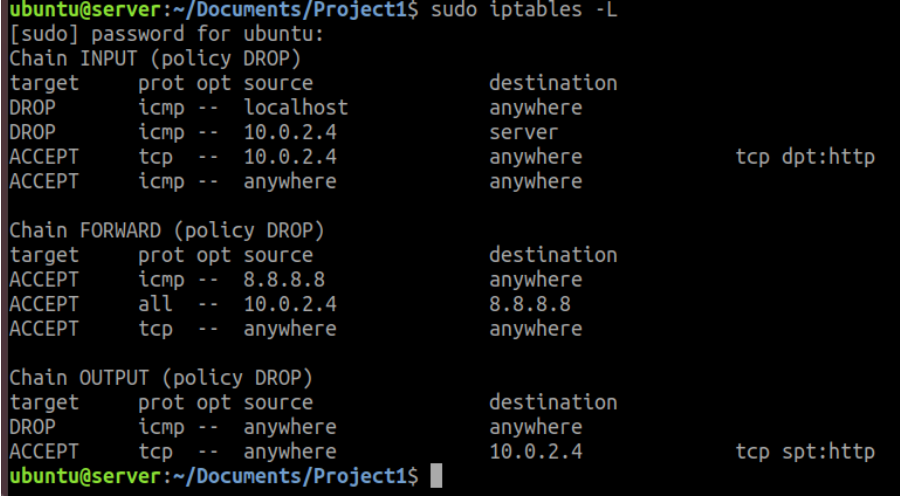
\includegraphics[width=0.7\linewidth]{files/CSE548_Fig_28-e6e4dc78bd01ccc2eb698abddc2ca988.png}
\caption[]{Gateway/Server's \texttt{iptables} Rules}
\label{CSE548_Fig_28}
\end{figure}

As can be seen in Figure~\ref{CSE548_Fig_28}: Gateway/Server's \texttt{iptables} Rules, the policy is of the ``whitelist'' type, where only allowed actions are authorized, and every other action is dropped.

\subparagraph{Project 2: SDN-Based Stateless Firewall Project}

New firewall rules were added to the Layer 3 and Layer 2 firewall configurations to container filtering rules per the Project instructions.  These are shown in Figure~\ref{CSE548_Fig_29}: Layer 3 Firewall Rules (rules 7 - 11 added) below:

\begin{figure}[!htbp]
\centering
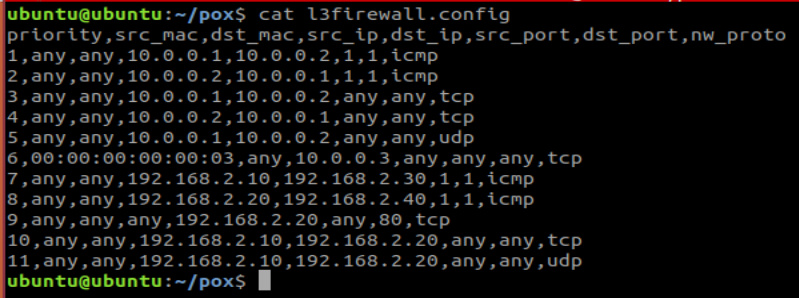
\includegraphics[width=0.7\linewidth]{files/CSE548_Fig_29-2f9fd7845ed67b0e54b3e33da2fc5965.png}
\caption[]{Layer 3 Firewall Rules (rules 7 - 11 added)}
\label{CSE548_Fig_29}
\end{figure}

Figure~\ref{CSE548_Fig_29}: Layer 3 Firewall Rules (rules 7 - 11 added) shows the Layer 3 firewall rules for the Open Virtual Switch.  To comply with the Project requirements, rules 7 through 11 were added.  These rules block:

\begin{itemize}
\item pinging beween Hosts 1 and 3
\item pinging between Hosts 2 and 4
\item block access to port 80 on Host 2
\item block any TCP or UDP traffic between Hosts 10 and 20
\end{itemize}

Layer 2 firewall rules were also implemented per the Project requirements.  The configuration of the Layer 2 firewall is shown in Figure~\ref{CSE548_Fig_30}: Layer 2 Firewall Rules (rule 3 added) below:

\begin{figure}[!htbp]
\centering
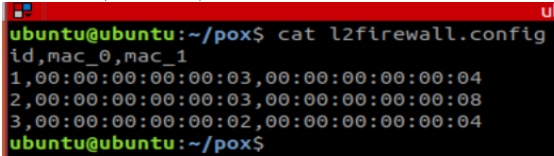
\includegraphics[width=0.7\linewidth]{files/CSE548_Fig_30-2a82b5f5a94a5c0f74b158b5a0a5e5ea.png}
\caption[]{Layer 2 Firewall Rules (rule 3 added)}
\label{CSE548_Fig_30}
\end{figure}

The additional rule created in the Layer 2 firewall shown in Figure~\ref{CSE548_Fig_30}: Layer 2 Firewall Rules (rule 3 added), blocks traffic by MAC address from Host 2 to Host 4.

\subparagraph{Project 3: SDN-Based DoS Attacks and Mitigation Project}

The aim of this project was to detect DoS attacks.  The first item that needs to be established is how to differentiate between normal and DoS traffic.  For nice round numbers, I have decided to use 10 connections in a 3 second time window.  The L3Firewall.py application was modified to include these new constants as shown in Figure~\ref{CSE548_Fig_31}: L3Firewall.py DoS Detection Threshold Constants below:

\begin{figure}[!htbp]
\centering
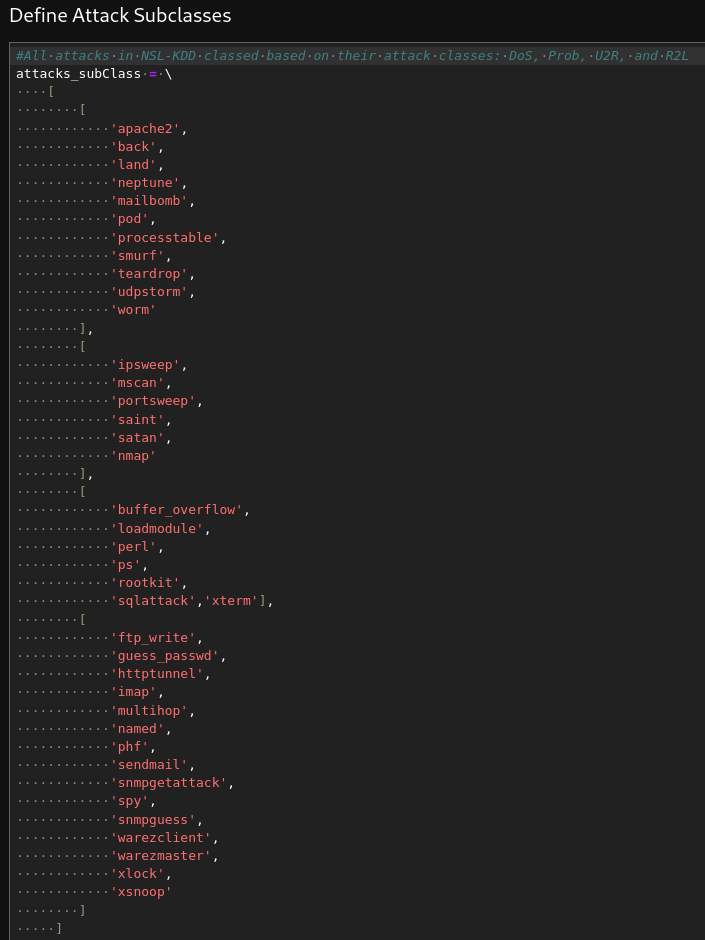
\includegraphics[width=0.7\linewidth]{files/CSE548_Fig_31-945f3308d8e4390eb108b99a15b33448.png}
\caption[]{L3Firewall.py DoS Detection Threshold Constants}
\label{CSE548_Fig_31}
\end{figure}

When examining the provided L3Firewall.py, I noticed that there was a function called:

\begin{verbatim}
replyToIP(self, packet, match, event, fwconfig)
\end{verbatim}

and it contained the logic for processing IP packets.  I therefore decided that the logic to detect a DoS style attack should go into this function.

The code that was added to the Program~\ref{CSE548_Code_1} function is shown in Program~\ref{CSE548_Code_2} below:

\begin{verbatim}
# ************* DDOS Mods start here *******************
log.debug("[*] Entered DDOS in replyToIP")
current_time = time.time()

# Create a new entry to track the new connection for possible offense
if srcmac not in connection_counter:
    connection_counter[srcmac] = []
connection_counter[srcmac].append(current_time)

# Clean up connections that don't meet offensive threshold		
connection_counter[srcmac] = \
    [item for item in connection_counter[srcmac] if (current_time - item) <= BLOCK_TIME_WINDOW]

# If the number of connections from the same MAC address exceeds the offense threshold, block.
if len(connection_counter[srcmac]) > BLOCK_THRESHOLD:
    log.debug("[*] Blocking MAC address %s for DDOS " % srcmac)
    self.blockMAC(event, srcmac)
    return
# ************* DDOS Mods end here *******************
\end{verbatim}

In the code snippet shown in Program~\ref{CSE548_Code_2}, an if statement checks whether or not a source MAC address is already in the \textit{connection\_counter} list of lists.  This list of lists contains a collection of MAC addresses that have not been seen before by the function and are now to be considered as possible DoS candidates.  If the source MAC is not in the \textit{connection\_counter} list of lists, then the current time is appended to the list corresponding to that source MAC address.

The next line is a list comprehension that removes any source MAC address whose connection time is greater than the \textit{BLOCK\_TIME\_WINDOW} constant, which is 3 seconds.  This constant was chosen heuristically in order to achieve reasonable results during testing.  Connections that exceed the  \textit{BLOCK\_TIME\_WINDOW} connection time are considered normal.

The next line is an if statement that checks if the length of the list for a particular source MAC address exceeds the \textit{BLOCK\_THRESHOLD} constant, which is 10 connection attempts.  If a particular source MAC address has 10 connections attempts, each lasting less than 3 seconds, then it is considered a source of DoS style attacks.  The source MAC is then sent to the Program~\ref{CSE548_Code_3} function, shown below:

\begin{verbatim}
# ************* My mods start here *******************
# Create function to block offending MAC address
def blockMAC(self, event, mac_address):
    # Add a flow rule to block a MAC address permanently
    log.debug("[*] Entered blockMAC")
    msg = of.ofp_flow_mod()
    match = of.ofp_match()
    match.dl_src = EthAddr(mac_address)
    match.dl_type = pkt.ethernet.IP_TYPE
    msg.match = match
    msg.priority = 65535 # high priority
    msg.action = []
    event.connection.send(msg)
    log.debug("[*] Permanently blocked the MAC address %s" % mac_address)
    log.debug("[*] Exiting blockMAC")
# ************* My mods end here ********************
\end{verbatim}

In the Program~\ref{CSE548_Code_3} function, code is present that sends a message to the OpenFlow controller's firewall to add an entry for the offending source MAC.  When this message is sent to the controller's firewall, the offending MAC address is blocked.

\subparagraph{Project 4: Machine Learning-Based Anomaly Detection Project}

In order to extract the specified scenarios from the provided training and testing datasets, a Python script called dataExtractor.py was provided by the course team.  This script was migrated into Jupyter Lab (see attachment \href{/sections/mcs-projects/mcs-portfolio-project/dataextractor}{Data Extractor}).  The script identifies the various attack classes and their associated subclasses as shown in Figure~\ref{CSE548_Fig_32}: Definition of Attack Subclasses below:

\begin{figure}[!htbp]
\centering
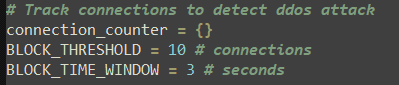
\includegraphics[width=0.7\linewidth]{files/CSE548_Fig_32-0a1912e68c0f314c886aba58d56b7f9f.png}
\caption[]{Definition of Attack Subclasses}
\label{CSE548_Fig_32}
\end{figure}

The training and testing datasets were loaded in memory as Pandas \footnote{Pandas. \href{https://pandas.pydata.org/}{https://pandas.pydata.org/}} dataframes.  A Pandas \href{https://pandas.pydata.org/pandas-docs/stable/reference/api/pandas.DataFrame.describe.html}{describe()} function was applied to the datasets to get an appreciation for their dimensions:

\begin{figure}[!htbp]
\centering
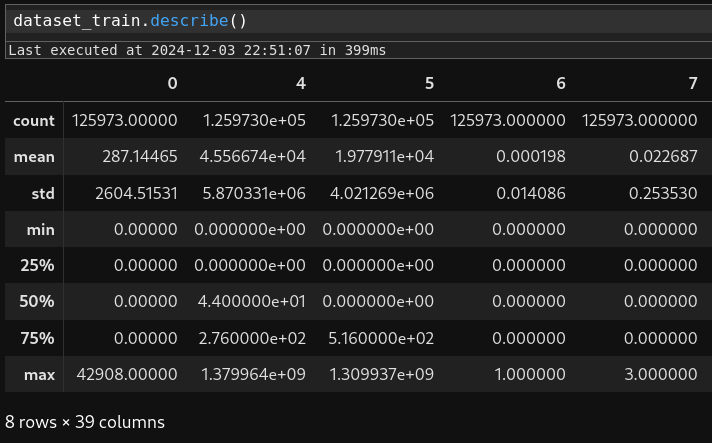
\includegraphics[width=0.7\linewidth]{files/CSE548_Fig_33-19f27524341961fff51ee02a75736fe3.png}
\caption[]{Training Dataset Characteristics (partial)}
\label{CSE548_Fig_33}
\end{figure}

Figure~\ref{CSE548_Fig_32}: Training Dataset Characteristics (partial) shows that the training dataset contains 125,973 rows of data.

\begin{figure}[!htbp]
\centering
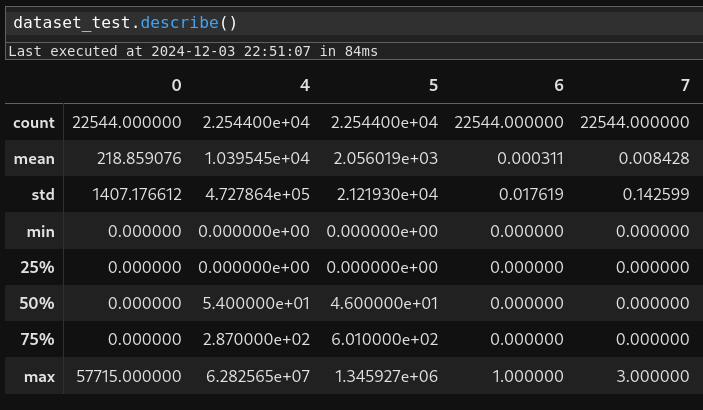
\includegraphics[width=0.7\linewidth]{files/CSE548_Fig_34-87d124a46ceb86dd70a73d8796c66b00.png}
\caption[]{Testing Dataset Characteristics (partial)}
\label{CSE548_Fig_34}
\end{figure}

Figure~\ref{CSE548_Fig_34}: Testing Dataset Characteristics (partial) shows that the testing dataset contains 22,544 rows of data.

Once the training and testing data are loaded into Pandas dataframes, they can be filtered for the desired training and testing data based on the three different scenarios as shown below:

\subparagraph{Scenario A Train / Test Configuration in Python}

\begin{verbatim}
attack_class_1 = [1, 3]
attack_class_1
\end{verbatim}

\begin{verbatim}
[1, 3]
\end{verbatim}

\begin{verbatim}
attack_class_2 = [2, 4]
attack_class_2
\end{verbatim}

\begin{verbatim}
[2, 4]
\end{verbatim}

\subparagraph{Scenario B Train / Test Configuration in Python}

\begin{verbatim}
attack_class_1 = [1, 2]
attack_class_1
\end{verbatim}

\begin{verbatim}
[1, 2]
\end{verbatim}

\begin{verbatim}
attack_class_2 = [1]
attack_class_2
\end{verbatim}

\begin{verbatim}
[1]
\end{verbatim}

\subparagraph{Scenario C Train / Test Configuration in Python}

\begin{verbatim}
attack_class_1 = [1, 2]
attack_class_1
\end{verbatim}

\begin{verbatim}
[1, 2]
\end{verbatim}

\begin{verbatim}
attack_class_2 = [1, 2, 3]
attack_class_2
\end{verbatim}

\begin{verbatim}
[1, 2, 3]
\end{verbatim}

For each scenario, a \textit{for} loop traverses the training and testing datasets and selects the desired attack classes.  Separated out training and testing datasets were then saved as CSV files for use in the next set of IPython \footnote{IPython. \href{https://ipython.org/}{https://ipython.org/}} Notebooks that perform the actual training and testing of the machine learning models.  For the A1 and A3 training datasets, this code cell is shown below in Training~A1~and~A3~Dataset~Generation:

\begin{verbatim}
print("Creating training set.....\n")
setA_train = []

if (training_attack_class_list[0][0] != 0) and \
    (len(training_attack_class_list[0]) != num_attack_class):

    for i in range(len(X_train)):
        # exp., X_train[i, -2] is the label of attack subclass, and attacks_subClass[training_attack_class_list[0][j] -1] identify the selected attack class
        if str.lower(str(X_train[i, -2])) == 'normal':
            setA_train.append(X_train[i])

        for j in range(len(training_attack_class_list[0])):
            if str.lower(str(X_train[i, -2])) in attacks_subClass[training_attack_class_list[0][j] -1]:
                setA_train.append(X_train[i])

    trainingFileName="Training"

    for i in range(len(training_attack_class_list[0])):
        trainingFileName = trainingFileName + " -a" + str(training_attack_class_list[0][i])

    trainingFileName = trainingFileName + file_extension

    np.savetxt(trainingFileName, setA_train, delimiter=',', fmt="%s" )

    print("Files " + trainingFileName + " have been created in the same folder this script resides\n")

elif (len(training_attack_class_list[0]) == num_attack_class):
    print("No changes is needed for training dataset!\n")
else:
    print("No attack classes are chosen, thus no new training file is created!\n")
\end{verbatim}

\begin{verbatim}
Creating training set.....

Files Training -a1 -a3.csv have been created in the same folder this script resides
\end{verbatim}

Similar methods were used to create the other training and testing datasets with subclasses per Table~\ref{CSE548_Table_1}: Train / Test Scenarios.

The created training and testing datasets were then imported into memory as Pandas dataframes.  Since the datasets contained both the features and labels, they needed to be further subdivided into training / testing features and labels.  The training features were extracted with the following code cell shown in Model~Training~Features below:

\begin{verbatim}
X_train = dataset_train.iloc[:, 0: -2].values
X_train
\end{verbatim}

\begin{verbatim}
array([[0, 'tcp', 'ftp_data', ..., 0.0, 0.05, 0.0],
       [0, 'udp', 'other', ..., 0.0, 0.0, 0.0],
       [0, 'tcp', 'private', ..., 1.0, 0.0, 0.0],
       ...,
       [0, 'tcp', 'smtp', ..., 0.0, 0.01, 0.0],
       [0, 'tcp', 'klogin', ..., 1.0, 0.0, 0.0],
       [0, 'tcp', 'ftp_data', ..., 0.0, 0.0, 0.0]], dtype=object)
\end{verbatim}

The training labels were extracted with the following code cell shown in below: Model~Training~Labels:

\begin{verbatim}
y_train = []
for i in range(len(label_column_train)):
    if label_column_train[i] == 'normal':
        y_train.append(0)
    else:
        y_train.append(1)

# Convert list to array
y_train = np.array(y_train)
\end{verbatim}

\begin{verbatim}
y_train
\end{verbatim}

\begin{verbatim}
array([0, 0, 1, ..., 0, 1, 0])
\end{verbatim}

We can see in Model~Training~Labels~Code that if the training label was `Normal' a `0' is appended; whereas if the label was a string other than `Normal' (i.e. some kind of attack), a `1' was appended.  Similar operations were performed for the testing data sets.  The training and testing features contained categorical data that needed to be converted into numeric data for model training and testing.  One -- Hot Encoding was selected as the method to perform this operation.  For the training feature dataset, the following code cells illustrates this operation:

\begin{verbatim}
# The following code work Python 3.7 or newer
from sklearn.preprocessing import OneHotEncoder
from sklearn.compose import ColumnTransformer
ct = ColumnTransformer(
     # The column numbers to be transformed ([1, 2, 3] represents three columns to be transferred)
    [('one_hot_encoder', OneHotEncoder(handle_unknown='ignore'), [1,2,3])],
    # Leave the rest of the columns untouched
    remainder='passthrough'
)
X_train = np.array(ct.fit_transform(X_train), dtype=np.float64)
X_test  = np.array(ct.transform(X_test) , dtype=np.float64)
\end{verbatim}

\begin{verbatim}
X_train
\end{verbatim}

\begin{verbatim}
array([[0.  , 1.  , 0.  , ..., 0.  , 0.05, 0.  ],
       [0.  , 0.  , 1.  , ..., 0.  , 0.  , 0.  ],
       [0.  , 1.  , 0.  , ..., 1.  , 0.  , 0.  ],
       ...,
       [0.  , 1.  , 0.  , ..., 0.  , 0.01, 0.  ],
       [0.  , 1.  , 0.  , ..., 1.  , 0.  , 0.  ],
       [0.  , 1.  , 0.  , ..., 0.  , 0.  , 0.  ]])
\end{verbatim}

In addition to dealing with categorical data, scaling was necessary to prevent a particular feature from over -- biasing the training data.  The \href{https://scikit-learn.org/stable/modules/generated/sklearn.preprocessing.StandardScaler.html}{SKLearn StandardScaler() class} was selected for this operation.  The code cells Perform~Feature~Scaling~on~Training~Data~Code and Perform~Feature~Scaling~on~Testing~Data~Code~Output show the results:

\begin{verbatim}
# Perform feature scaling. For ANN you can use StandardScaler, for RNNs recommended is 
# MinMaxScaler. 
# referece: https://scikit -learn.org/stable/modules/generated/sklearn.preprocessing.StandardScaler.html
# https://scikit -learn.org/stable/modules/preprocessing.html
from sklearn.preprocessing import StandardScaler
sc = StandardScaler()
X_train = sc.fit_transform(X_train)  # Scaling to the range [0,1]
X_test  = sc.fit_transform(X_test)
\end{verbatim}

\begin{verbatim}
X_train
\end{verbatim}

\begin{verbatim}
array([[ -0.19511653,  0.42713604, -0.36510181, ..., -0.66659951,
        -0.14895839, -0.31810766],
       [ -0.19511653, -2.34117451,  2.73896205, ..., -0.66659951,
        -0.32815058, -0.31810766],
       [ -0.19511653,  0.42713604, -0.36510181, ...,  1.51653833,
        -0.32815058, -0.31810766],
       ...,
       [ -0.19511653,  0.42713604, -0.36510181, ..., -0.66659951,
        -0.29231215, -0.31810766],
       [ -0.19511653,  0.42713604, -0.36510181, ...,  1.51653833,
        -0.32815058, -0.31810766],
       [ -0.19511653,  0.42713604, -0.36510181, ..., -0.66659951,
        -0.32815058, -0.31810766]])
\end{verbatim}

The training features are now normalized with a mean of zero.  A similar operation was performed for the testing data.

Once the training and testing data are cleaned and prepared, a Fully -- connected Neural Network (FNN) can be constructed.  The FNN is defined as shown in the Defining~FNN~Structure code cell below:

\begin{verbatim}
# Adding the input layer and the first hidden layer, 6 nodes, input_dim specifies the number of variables
# rectified linear unit activation function relu, reference: https://machinelearningmastery.com/rectified -linear -activation -function -for -deep -learning -neural -networks/
# Adding the input layer with Input() and the first hidden layer
classifier.add(Input(shape=(len(X_train[0]),)))  # Input layer
classifier.add(Dense(units=6, kernel_initializer='uniform', activation='relu'))

# Adding the second hidden layer
classifier.add(Dense(units=6, kernel_initializer='uniform', activation='relu'))

# Adding the output layer
classifier.add(Dense(units=1, kernel_initializer='uniform', activation='sigmoid'))
\end{verbatim}

\begin{framed}
\textbf{Additional Context from Copilot}\\
In the Defining~FNN~Structure code cell, we can see that the FNN has an input layer of 6 neurons, a hidden layer of 6 neurons and an output layer of one neuron.  The activation function for the hidden layer is ReLU (Rectified Linear Unit), and the activation function for the output layer is Sigmoid.
\end{framed}

The model was compiled with the parameters as shown in the Compilation~of~FNN code cell below:

\begin{verbatim}
# Compiling the ANN, 

# Gradient descent algorithm “adam“, Reference: https://machinelearningmastery.com/adam -optimization -algorithm -for -deep -learning/

# This loss is for a binary classification problems and is defined in Keras as “binary_crossentropy“, Reference: https://machinelearningmastery.com/how -to -choose -loss -functions -when -training -deep -learning -neural -networks/

classifier.compile(
    optimizer = 'adam', 
    loss = 'binary_crossentropy', 
    metrics = ['accuracy']
    )
\end{verbatim}

\begin{framed}
\textbf{Website Referenced in Defining~FNN~Structure and Compilation~of~FNN}\\
The code for defining and compiling the FNN was inspired by the following website:
\href{https://machinelearningmastery.com}{https://machinelearningmastery.com}
\end{framed}

In Compilation~of~FNN, we can see that the FNN was compiled with the ADAM optimizer, a `binary\_crossentropy' loss function, and the metric is `accuracy'.  The choices for these hyperparameters were made based on the provided code from the Course team.

\begin{framed}
\textbf{Additional Context from Copilot}\\
\begin{itemize}
\item \texttt{ADAM} optimizer: an adaptive first‑and‑second‑moment SGD (momentum + RMSProp) optimizer (good default; typically uses lr=0.001) that speeds and stabilizes training.
\item \texttt{binary\_crossentropy} loss: the log loss for binary targets; for a true label y∈\{0,1\} and predicted probability p, loss = $- \big(y\log p + (1 -y)\log(1 -p)\big)$. It's appropriate for a single-output sigmoid FNN.
\item \texttt{accuracy} metric: fraction of examples classified correctly (Keras uses a default 0.5 threshold on the sigmoid output).
\end{itemize}
\end{framed}

The model was then fit and saved as a Keras file.  This was done to avoid retraining the model during code development since model trainnig takes a very long time. The code cell Train~Model Save~Model~to~Keras~Fileshows the code cells that perform the training and saving of the traning history data.

\begin{verbatim}
# Fitting the ANN to the Training set
# Train the model so that it learns a good (or good enough) mapping of rows of input data to the output classification.
# add verbose=0 to turn off the progress report during the training
# To run the whole training dataset as one Batch, assign batch size: BatchSize=X_train.shape[0#]
#classifierHistory = classifier.fit(X_train, y_train, batch_size = BatchSize, epochs = NumEpoch)
\end{verbatim}

\begin{verbatim}
Epoch 1/10
11333/11333 [==============================] - 26s 2ms/step - loss: 0.0347 - accuracy: 0.9885
Epoch 2/10
11333/11333 [==============================] - 26s 2ms/step - loss: 0.0137 - accuracy: 0.9960
Epoch 3/10
11333/11333 [==============================] - 25s 2ms/step - loss: 0.0106 - accuracy: 0.9969
Epoch 4/10
11333/11333 [==============================] - 25s 2ms/step - loss: 0.0095 - accuracy: 0.9974
Epoch 5/10
11333/11333 [==============================] - 26s 2ms/step - loss: 0.0084 - accuracy: 0.9977
Epoch 6/10
11333/11333 [==============================] - 26s 2ms/step - loss: 0.0076 - accuracy: 0.9979
Epoch 7/10
11333/11333 [==============================] - 26s 2ms/step - loss: 0.0071 - accuracy: 0.9981
Epoch 8/10
11333/11333 [==============================] - 25s 2ms/step - loss: 0.0068 - accuracy: 0.9981
Epoch 9/10
11333/11333 [==============================] - 25s 2ms/step - loss: 0.0067 - accuracy: 0.9981
Epoch 10/10
11333/11333 [==============================] - 26s 2ms/step - loss: 0.0067 - accuracy: 0.9982
\end{verbatim}

\begin{verbatim}
classifier.save("fitted_FNN_model_SA.keras")  # Save the model in HDF5 format

# Save the history
#import json
#with open("fitted_FNN_model_history_SA.json", "w") as f:
#    json.dump(classifierHistory.history, f)
\end{verbatim}

\begin{framed}
\textbf{Note}\\
In the code cell Train~Model, the command \href{http://classifier.fit}{classifier.fit}() is commented out to avoid retraining the model during code development.  The trained model is saved as shown in the code cell Save~Model~to~Keras~File and is recalled from the Keras file in the code cell Load~Model~from~Keras~File~and~Load~Training~History~from~JSON~File.
\end{framed}

Once the model was trained, it can be reloaded at any time using the Keras load\_model() function.  The model's training history is loaded from a JSON file.  The following code cell in Load~Model~from~Keras~File~and~Load~Training~History~from~JSON~File displays this process:

\begin{verbatim}
#from keras.models import load_model

#classifier = load_model("fitted_FNN_model_SA.keras")  # Load the saved model

# Load the history
#import json
#with open("fitted_FNN_model_history_SA.json", "r") as f:
#    classifierHistory = json.load(f)
\end{verbatim}

\begin{framed}
\textbf{Note}\\
In the code cell Load~Model~from~Keras~File~and~Load~Training~History~from~JSON~File, the commands are commented out to avoid overwriting the trained model and training history during code development.
\end{framed}

Similar operations were performed for all Scenarios.  Now that the models are trained, they can be tested per the conditions described in Table~\ref{CSE548_Table_1}.

\subparagraph{Description of Results}

\subparagraph{Project 1: Packet Filter Firewall (iptables) Project}

Once the webserver was setup on the Gateway/Server, accessing the webpage using the Linux command \href{https://www.man7.org/linux/man-pages/man1/curl.1.html}{curl} from the client was possible.  This is shown in Figure~\ref{CSE548_Fig_35}: Accessing the Web Server on the Gateway/Server from the Client below:

\begin{figure}[!htbp]
\centering
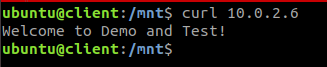
\includegraphics[width=0.7\linewidth]{files/CSE548_Fig_35-df9d0232a83a259487a0d1c2daebc129.png}
\caption[]{Accessing the Web Server on the Gateway/Server from the Client}
\label{CSE548_Fig_35}
\end{figure}

In order to test proper functioning of the firewall, the following port scans were performed as shown in Figure~\ref{CSE548_Fig_36}: Client TCP Port Scan of Server and Figure~\ref{CSE548_Fig_37}: Client UDP Port Scan of Server:

\subparagraph{Client TCP Port Scan of Server}

\begin{figure}[!htbp]
\centering
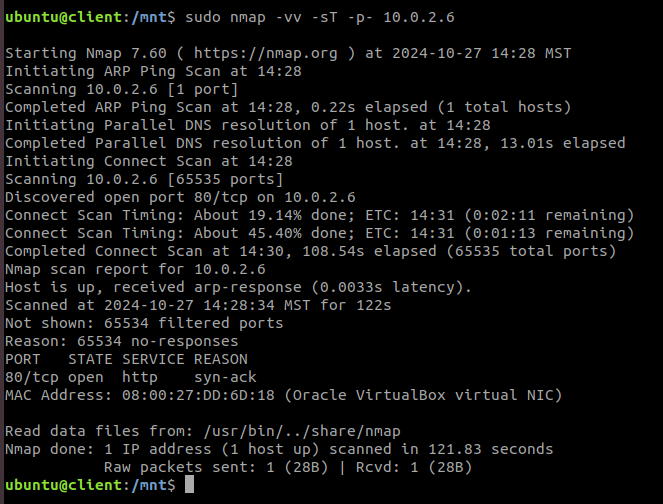
\includegraphics[width=0.7\linewidth]{files/CSE548_Fig_36-be325bc9c29316cc6c40a06dba414673.png}
\caption[]{Client TCP Port Scan of Server}
\label{CSE548_Fig_36}
\end{figure}

\subparagraph{Client UDP Port Scan of Server}

\begin{figure}[!htbp]
\centering
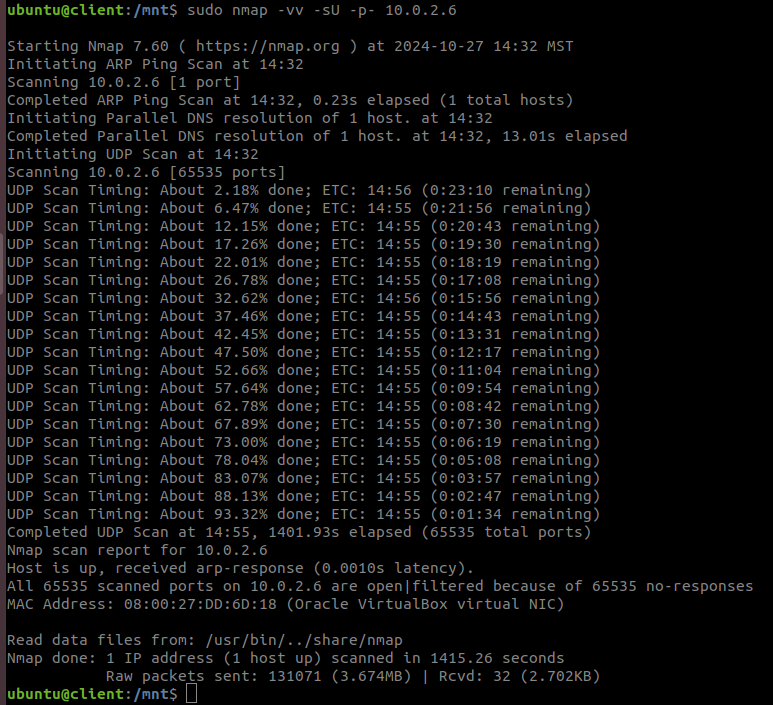
\includegraphics[width=0.7\linewidth]{files/CSE548_Fig_37-0a122268d474022b0bb53bb3e9c21c20.png}
\caption[]{Client UDP Port Scan of Server}
\label{CSE548_Fig_37}
\end{figure}

In Figure~\ref{CSE548_Fig_36}: Client TCP Port Scan of Server we can see that because of the firewall (iptables) rules, the only TCP port the client can have access to is port 80 on the Gateway/Server.  Figure~\ref{CSE548_Fig_37}: Client UDP Port Scan of Server shows that all UDP ports on the Gateway/Server are closed to the Client as per Project Requirements.

\subparagraph{Ping Tests to Verify Firewall Requirements}

Another requirement of the Project is that the Client must be able to ping 8.8.8.8.  For this to work, the Gateway/Server needs to be setup as the default gateway on the Client, and the Gateway/Server must implement Network Address Translation to translate ICMP\footnote{Internet Control Message Protocol (ICMP). \href{https://en.wikipedia.org/wiki/Internet\_Control\_Message\_Protocol}{Internet Control Message Protocol}, \href{https://tools.ietf.org/html/rfc792}{https://tools.ietf.org/html/rfc792}} send and receive packets from 8.8.8.8 to and from the Client, respectively.  The Client was able to send pings to 8.8.8.8 successfully and the results are shown in Figure~\ref{CSE548_Fig_38}: Client Ping to Internet Address 8.8.8.8 below:

\begin{figure}[!htbp]
\centering
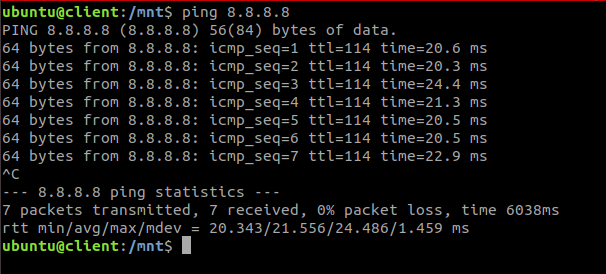
\includegraphics[width=0.7\linewidth]{files/CSE548_Fig_38-bab70c8ddb3a60f2e4da1f3dad464816.png}
\caption[]{Client Ping to Internet Address 8.8.8.8}
\label{CSE548_Fig_38}
\end{figure}

A Project requirement is that the Client must not be able to ping to 8.8.4.4.  Since there is no explicit whitelist rule allowing pings to this address, the ICMP ping packets were dropped as required.  This is shown in Figure~\ref{CSE548_Fig_39}: Client Ping to Internet Address 8.8.4.4 below:

\begin{figure}[!htbp]
\centering
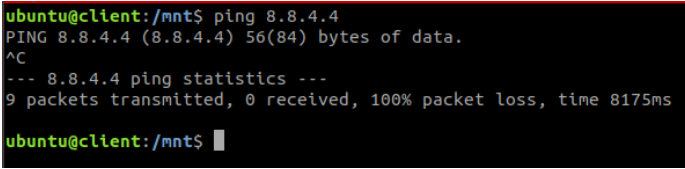
\includegraphics[width=0.7\linewidth]{files/CSE548_Fig_39-b09714c70c9756480d861b70be1e9bd2.png}
\caption[]{Client Ping to Internet Address 8.8.4.4}
\label{CSE548_Fig_39}
\end{figure}

A Project requirement is that the Client must not be able to ping the Gateway/Server.  The firewall on the Gateway/Server was setup to drop ping packets from the Client.  Successful test results of this are shown in Figure~\ref{CSE548_Fig_40}: Client Ping of Gateway/Server below:

\begin{figure}[!htbp]
\centering
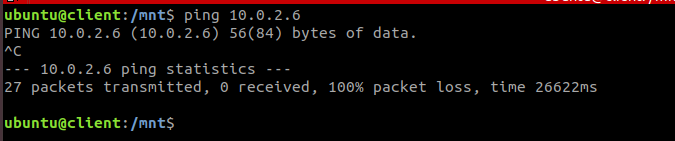
\includegraphics[width=0.7\linewidth]{files/CSE548_Fig_40-c767609086f627e5f839dfb9d9d70737.png}
\caption[]{Client Ping of Gateway/Server}
\label{CSE548_Fig_40}
\end{figure}

A Project requirement is that the Gateway/Server must not be able to ping the localhost.  ICMP packets that are sent from the Server and outside of the whitelist are successfully blocked as shown in Figure~\ref{CSE548_Fig_41}: Server Ping to Localhost below:

\begin{figure}[!htbp]
\centering
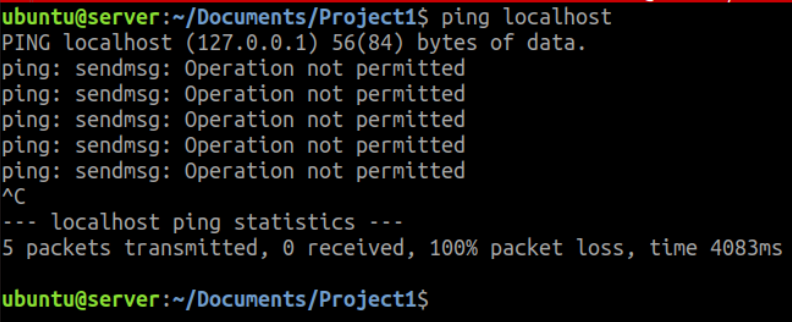
\includegraphics[width=0.7\linewidth]{files/CSE548_Fig_41-7b25f66d8621cb85ff1fdc2315501ab9.png}
\caption[]{Server Ping to Localhost}
\label{CSE548_Fig_41}
\end{figure}

A Project requirement is that the Gateway/Server must not be able to ping the Client.  ICMP packets that are sent from the Server and outside of the whitelist are successfully blocked as shown in Figure~\ref{CSE548_Fig_42}: Server Ping to Client below:

\begin{figure}[!htbp]
\centering
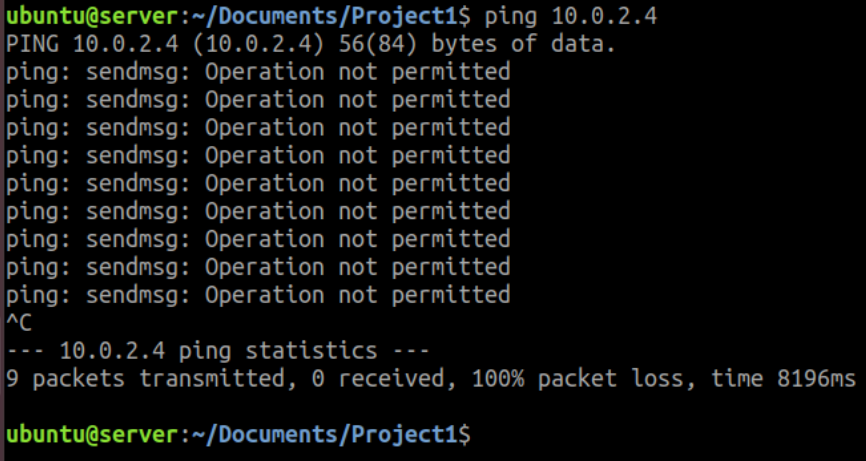
\includegraphics[width=0.7\linewidth]{files/CSE548_Fig_42-a7b548f15711a4dc9f9310fd503c4f14.png}
\caption[]{Server Ping to Client}
\label{CSE548_Fig_42}
\end{figure}

\subparagraph{Project 2: SDN-Based Stateless Firewall Project}

Once the firewalls were setup on the Controller, pings were blocked per the Project requirements.  For example, when Host 1 tried to ping Host 3, the pings were dropped, as shown in Figure~\ref{CSE548_Fig_43}: Check Blocking ICMP Traffic from 192.168.2.10 to 192.168.2.30 below:

\begin{figure}[!htbp]
\centering
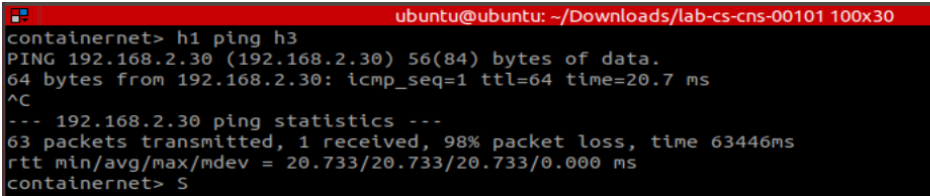
\includegraphics[width=0.7\linewidth]{files/CSE548_Fig_43-b0c7d9509c50afb08477d70c41983280.png}
\caption[]{Check Blocking ICMP Traffic from 192.168.2.10 to 192.168.2.30}
\label{CSE548_Fig_43}
\end{figure}

Note that in Figure~\ref{CSE548_Fig_43}: Check Blocking ICMP Traffic from 192.168.2.10 to 192.168.2.30, we can see that one ping did go through, but then the learning firewall learned the flow rule to block the remaining ping packets.  A similar successful test was performed for pings from Host 2 to Host 4 per Project requirements.  The results are shown in Figure~\ref{CSE548_Fig_44}: Check Blocking ICMP Traffic from 192.168.2.20 to 192.168.2.40 below:

\begin{figure}[!htbp]
\centering
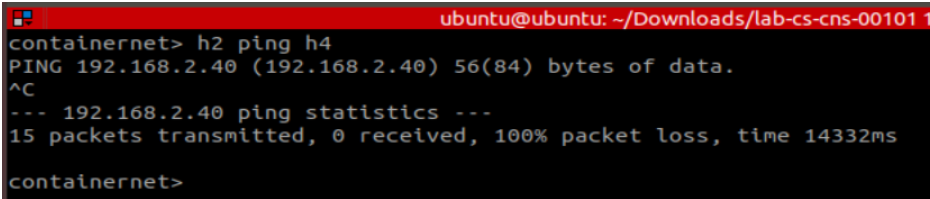
\includegraphics[width=0.7\linewidth]{files/CSE548_Fig_44-ad652011d30de12c22f6fbc78c6ff008.png}
\caption[]{Check Blocking ICMP Traffic from 192.168.2.20 to 192.168.2.40}
\label{CSE548_Fig_44}
\end{figure}

A Project requirement is that HTTP traffic must be blocked from Host 2 to any requestor.  To test this flow rule, the \href{https://pythonbasics.org/webserver/}{Python Simple Webserver} was started on Host 2 (Figure~\ref{CSE548_Fig_45}: HTTP Server Setup on Host 2).  A successful test of HTTP requests being blocked from the three other Hosts are shown in Figure~\ref{CSE548_Fig_46}: HTTP Requests to Node 2 Blocked below:

\begin{figure}[!htbp]
\centering
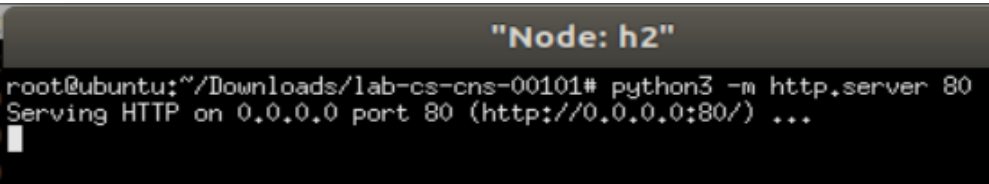
\includegraphics[width=0.7\linewidth]{files/CSE548_Fig_45-d0bc46e5c51d40ee743540aa2ae1d119.png}
\caption[]{HTTP Server Setup on Host 2}
\label{CSE548_Fig_45}
\end{figure}

\begin{figure}[!htbp]
\centering
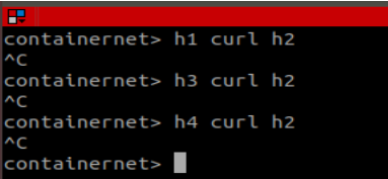
\includegraphics[width=0.7\linewidth]{files/CSE548_Fig_46-bff2a2fc33dc5995a51537fa7ae8772d.png}
\caption[]{HTTP Requests to Node 2 Blocked}
\label{CSE548_Fig_46}
\end{figure}

A Project requirement is that MAC address filtering is performed from Host 2 to Host 4.  To perform this test, the Linux command \href{https://linux.die.net/man/8/arping}{arping} was used.  A successful test showing the MAC address filtering from Host 2 to Host 4 was performed and the results are shown in Figure~\ref{CSE548_Fig_47}: Host 2 to Host 4 MAC Address Filtering below:

\begin{figure}[!htbp]
\centering
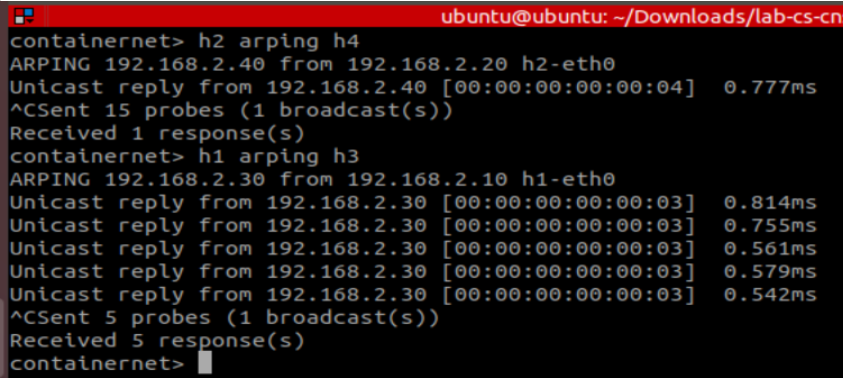
\includegraphics[width=0.7\linewidth]{files/CSE548_Fig_47-b0806778c17c73742e8ac4e32d8f7fd3.png}
\caption[]{Host 2 to Host 4 MAC Address Filtering}
\label{CSE548_Fig_47}
\end{figure}

It can be seen in Figure~\ref{CSE548_Fig_47}: Host 2 to Host 4 MAC Address Filtering that only one response is received from Node 4, while testing \href{https://linux.die.net/man/8/arping}{arping} from Node 1 to Node 3 produced many responses.  This is taken as traffic from Node 2 to Node 4 is blocked based on MAC addresses, since the first reply is necessary for the Controller to learn the flow rule.

A Project requirement is that both TCP and UDP traffic are blocked from Host 1 to Host 2.  The \href{https://linux.die.net/man/8/hping3}{hping3} Linux command was used to send both TCP and UDP packets.  A successful test of TCP packets being blocked when sent from Host 1 to Host 2 is shown in Figure~\ref{CSE548_Fig_48}: Check Blocking of TCP Traffic from Host 1 to Host 2 below:

\begin{figure}[!htbp]
\centering
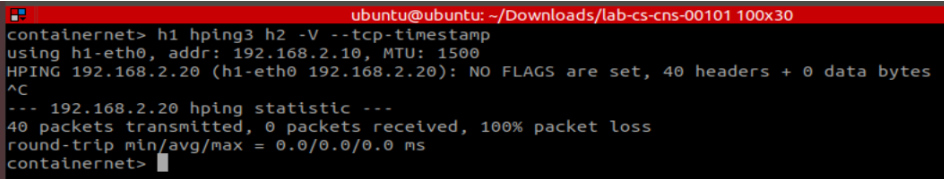
\includegraphics[width=0.7\linewidth]{files/CSE548_Fig_48-cef2716dcedb686f4cf1589f0f99d0b9.png}
\caption[]{Check Blocking of TCP Traffic from Host 1 to Host 2}
\label{CSE548_Fig_48   }
\end{figure}

Likewise, for UDP traffic, a successful test showing that the UDP traffic from Host 1 to Host 2 is being blocked is shown in Figure~\ref{CSE548_Fig_49}: Check Blocking of UDP Traffic from Host 1 to Host 2 below:

\begin{figure}[!htbp]
\centering
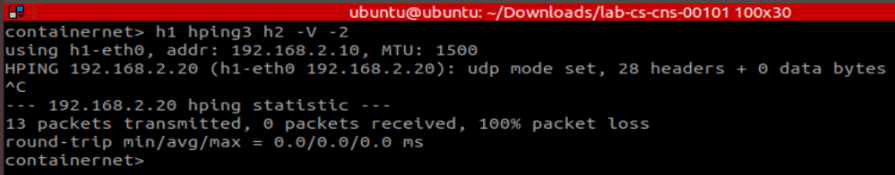
\includegraphics[width=0.7\linewidth]{files/CSE548_Fig_49-3c9213dd9c8254b5dbad072366962a4a.png}
\caption[]{Check Blocking of UDP Traffic from Host 1 to Host 2}
\label{CSE548_Fig_49}
\end{figure}

As can be seen from Figure~\ref{CSE548_Fig_48}: Check Blocking of TCP Traffic from Host 1 to Host 2 and Figure~\ref{CSE548_Fig_49}: Check Blocking of UDP Traffic from Host 1 to Host 2, both TCP and UDP traffic was successfully blocked from Host 1 to Host 2.

\subparagraph{Project 3: SDN-Based DoS Attacks and Mitigation Project}

As a baseline, a DoS flood test was performed from Host 1 to 192.168.2.20 (Host 2) with a spoofed source address of 10.10.10.1.  The commands used to initiate the flood test are shown in Figure~\ref{CSE548_Fig_50}: Packet Flood Test from Host 1 to Host 2 with Spoofed Source IP Address 10.10.10.1 below:

\begin{figure}[!htbp]
\centering
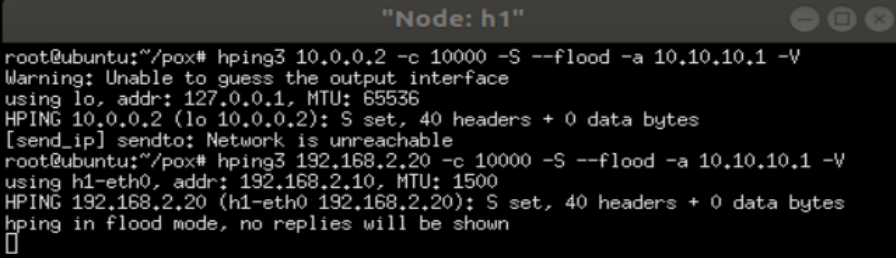
\includegraphics[width=0.7\linewidth]{files/CSE548_Fig_50-1404f3fc2b83b63b16fc89ff72ca4feb.png}
\caption[]{Packet Flood Test from Host 1 to Host 2 with Spoofed Source IP Address}
\label{CSE548_Fig_50}
\end{figure}

\begin{framed}
\textbf{Explanation of hping3 Command by Copilot}\\
The command used in Figure~\ref{CSE548_Fig_50}: Packet Flood Test from Host 1 to Host 2 with Spoofed Source IP Address is:
\texttt{hping3 10.0.0.2 -c 10000 -S --flood -a 10.10.10.1 -V}

\begin{itemize}
\item \texttt{10.0.0.2}: target IP.
\item \texttt{-c 10000}: send (up to) 10,000 packets then exit.
\item \texttt{-S}: set the TCP SYN flag (crafts SYN packets).
\item \texttt{--flood}: send packets as fast as possible (no delays), i.e., a high‑rate send.
\item \texttt{-a 10.10.10.1}: spoof the source IP address to 10.10.10.1.
\item \texttt{-V}: verbose output (show packet headers/info).
\end{itemize}

Summary: this issues a high‑rate SYN flood (DoS-style) toward 10.0.0.2 while spoofing the source IP. It requires root privileges, can disrupt networks/hosts, and may be illegal or against policy if run against systems you do not own --- do not run this on networks without explicit authorization.
\end{framed}

As the flood of packets was happening, the OpenFlow switch's flow entries were updating in real time as shown in Figure~\ref{CSE548_Fig_51}: OpenFlow Entries during Packet Flood below:

\begin{figure}[!htbp]
\centering
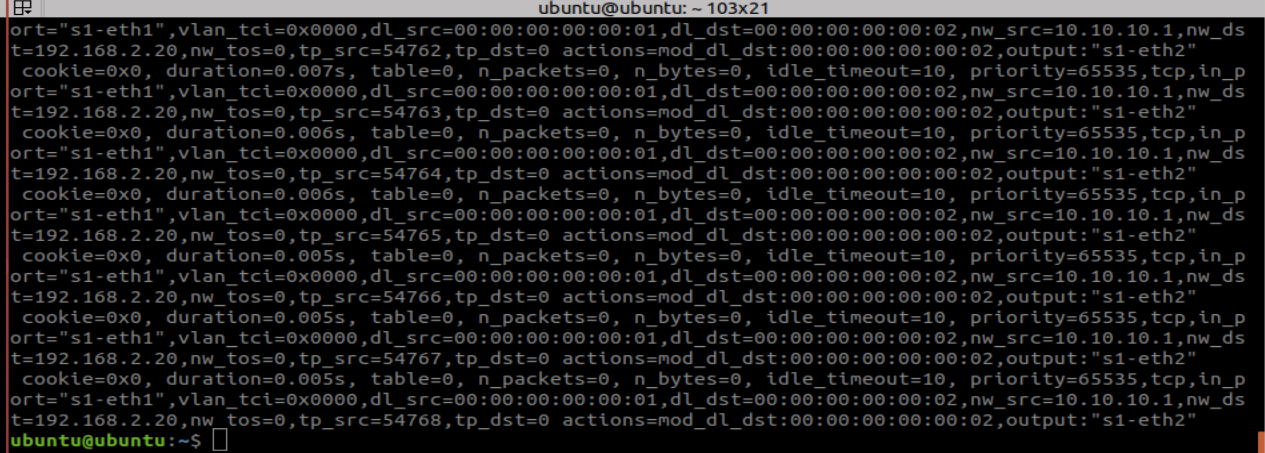
\includegraphics[width=0.7\linewidth]{files/CSE548_Fig_51-c009cd7c15f52399986e5795fca4cc9d.png}
\caption[]{OpenFlow Entries during Packet Flood}
\label{CSE548_Fig_51}
\end{figure}

The POX controller window was also displaying learned flow rules as shown in Figure~\ref{CSE548_Fig_52}: POX Controller Output during Packet Flood below:

\begin{figure}[!htbp]
\centering
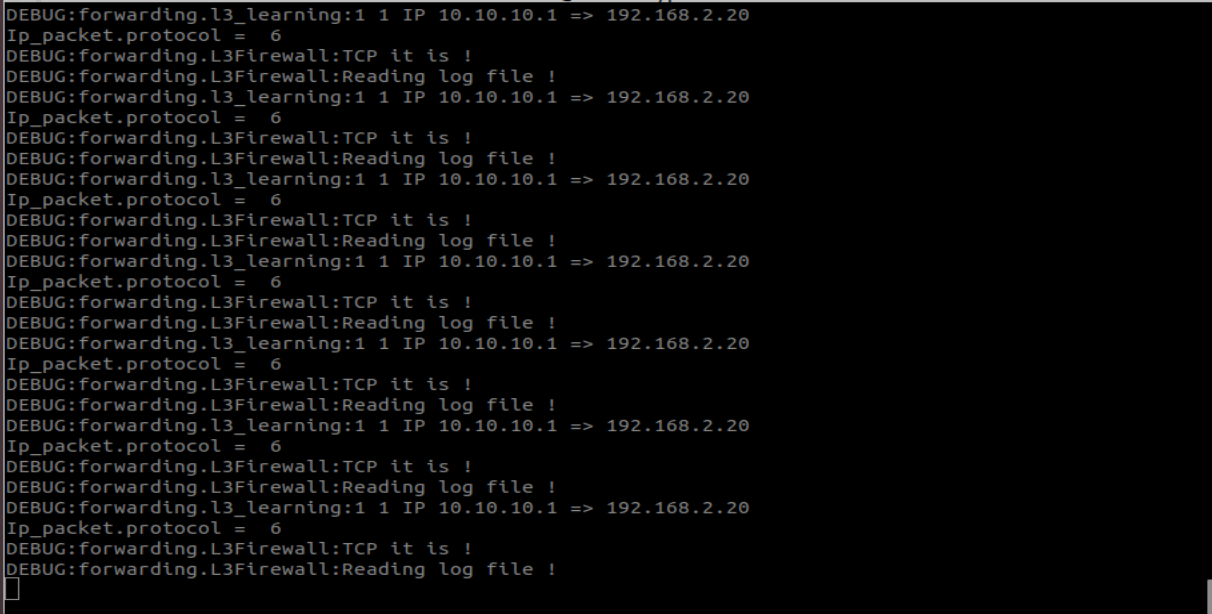
\includegraphics[width=0.7\linewidth]{files/CSE548_Fig_52-c074d12bc12a8765982d047dc9a247c8.png}
\caption[]{POX Controller Output during Packet Flood}
\label{CSE548_Fig_52}
\end{figure}

We used the \href{https://github.com/iptraf-ng/iptraf-ng}{iptraf-ng}\footnote{\texttt{iptraf-ng} is an ncurses-based IP LAN monitor that generates various network statistics including TCP info, UDP counts, ICMP   and OSPF information, Ethernet load info, node stats, IP checksum errors, and others.  If the \texttt{iptraf-ng} command is issued without any command-line options, the program comes up in interactive mode, with the various facilities accessed through the main menu. \href{https://www.man7.org/linux/man-pages/man8/iptraf-ng.8.html}{https://www.man7.org/linux/man-pages/man8/iptraf-ng.8.html}, \href{https://github.com/iptraf-ng/iptraf-ng}{https://github.com/iptraf-ng/iptraf-ng}} Linux application to monitor the amount of IP packets during the packet flood.  The output of \href{https://github.com/iptraf-ng/iptraf-ng}{iptraf-ng} is shown in Figure~\ref{CSE548_Fig_53}: Iptraf-ng Output during Packet Flood below:

\begin{figure}[!htbp]
\centering
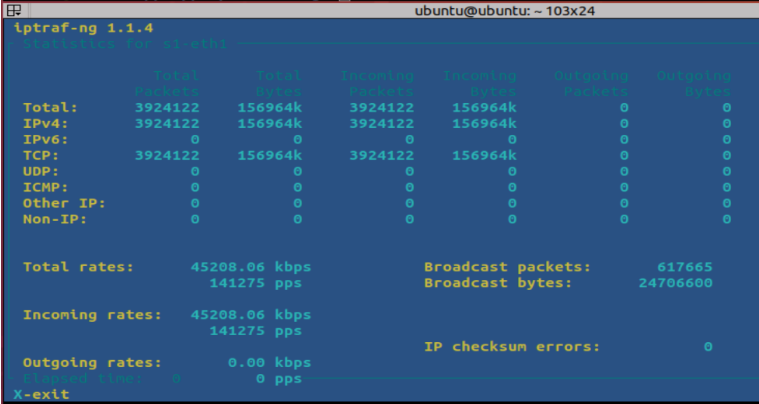
\includegraphics[width=0.7\linewidth]{files/CSE548_Fig_53-32eaedd1a6ee3e72935f0b321fca8620.png}
\caption[]{Iptraf-ng Output during Packet Flood}
\label{CSE548_Fig_53}
\end{figure}

It can be seen from Figure~\ref{CSE548_Fig_53}: Iptraf-ng Output during Packet Flood that a huge amount of packets were being sent and a DoS attack was successful.

To mitigate the DoS attack, I swapped out the baseline L3Firewall.py for my modified version and restarted the POX controller.  Again, a DoS was started as shown in Figure~\ref{CSE548_Fig_54}: DoS Attack from Host 1 to Host 2 with Spoofed Source Address of 10.10.10.1 below:

\begin{figure}[!htbp]
\centering
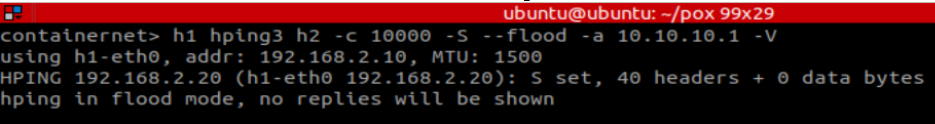
\includegraphics[width=0.7\linewidth]{files/CSE548_Fig_54-53a211b2c476097422a931150133036b.png}
\caption[]{DoS Attack from Host 1 to Host 2 with Spoofed Source Address of 10.10.10.1}
\label{CSE548_Fig_54}
\end{figure}

As before, we observed the traffic flows on the OpenFlow switch.  The observation was performed using the Linux \href{https://www.man7.org/linux/man-pages/man1/watch.1.html}{watch}\footnote{\texttt{watch} runs command repeatedly, displaying its output and errors (the first screenful). This allows you to watch the program output change over time. By default, command is run every 2 seconds and \texttt{watch} will run until interrupted.  A header informs of the start and running time of command as well as its exit code. \href{https://www.man7.org/linux/man-pages/man1/watch.1.html}{https://www.man7.org/linux/man-pages/man1/watch.1.html}} command, so as to be able to observe changes more easily without having to notice changes in a rapidly scrolling screen.  The results of the Linux \href{https://www.man7.org/linux/man-pages/man1/watch.1.html}{watch} command are shown in Figure~\ref{CSE548_Fig_55}: Watch of OpenFlow Switch Traffic Flows.  We notice that a flow rule was added to drop packets from MAC address ending in 01 (i.e. the offending MAC address).

\begin{figure}[!htbp]
\centering
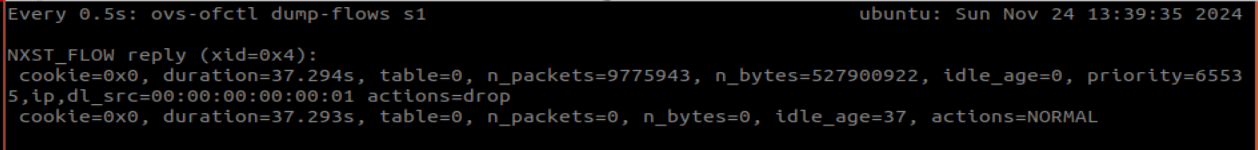
\includegraphics[width=0.7\linewidth]{files/CSE548_Fig_55-9d3f85b265e2d11b139ca547ec84c4ba.png}
\caption[]{Watch of OpenFlow Switch Traffic Flows}
\label{CSE548_Fig_55}
\end{figure}

The output of the POX controller indicates that a MAC address was blocked.  This is shown in Figure~\ref{CSE548_Fig_56}: POX Controller Output Indicating Offending MAC Address Permanently Blocked below:

\begin{figure}[!htbp]
\centering
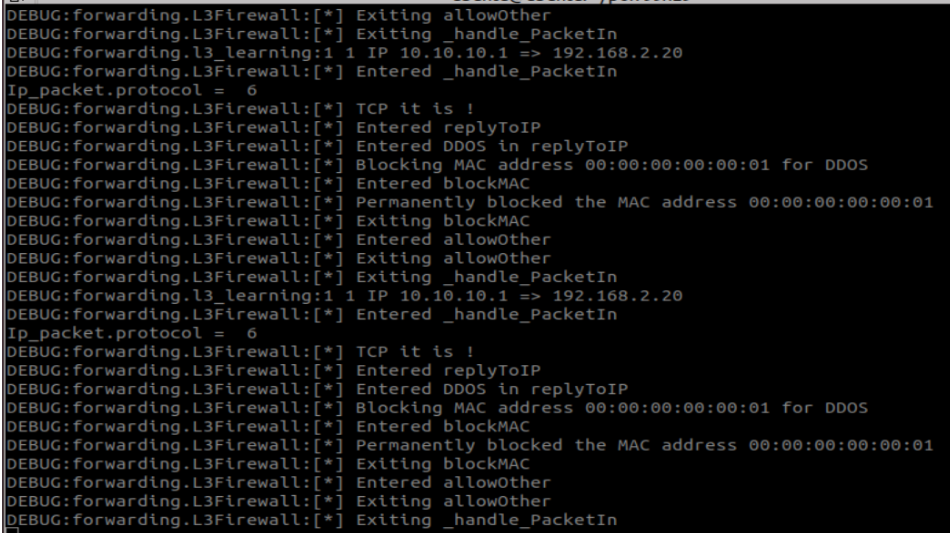
\includegraphics[width=0.7\linewidth]{files/CSE548_Fig_56-350e457c701378ea9f620c27ffc18223.png}
\caption[]{POX Controller Output Indicating Offending MAC Address Permanently Blocked}
\label{CSE548_Fig_56}
\end{figure}

Pinging between other hosts is still possible as the switch blocks the DoS attack from Host 1.  For example pinging from Host 4 to Host 3 is shown below in Figure~\ref{CSE548_Fig_57}: Pinging Allowed Between Host 4 and Host 3:

\begin{figure}[!htbp]
\centering
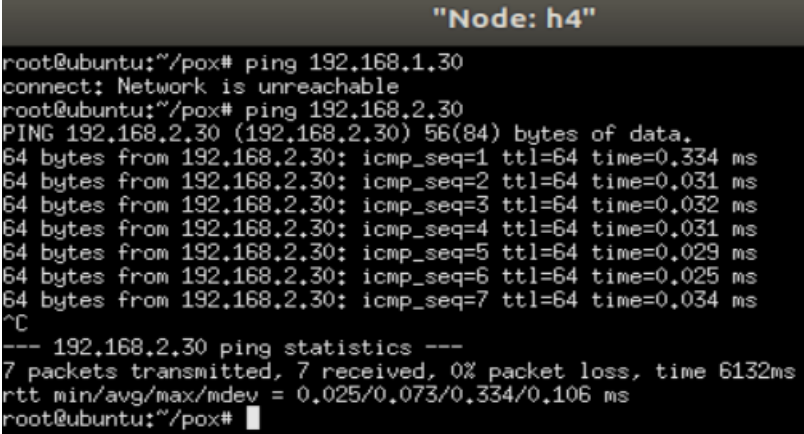
\includegraphics[width=0.7\linewidth]{files/CSE548_Fig_57-7dfd469b75980042cc00c1270da349e5.png}
\caption[]{Pinging Allowed Between Host 4 and Host 3}
\label{CSE548_Fig_57}
\end{figure}

However, pinging from Host 1 to any other host is blocked, as shown in Figure~\ref{CSE548_Fig_58}: Pings Blocked from Host 1 to Any Other Host, Figure~\ref{CSE548_Fig_59}: Pings Blocked from Host 1 to Any Other Host, and Figure~\ref{CSE548_Fig_60}: Pings Blocked from Host 1 to Any Other Host below:

\begin{figure}[!htbp]
\centering
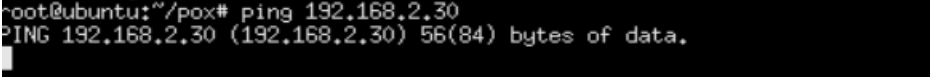
\includegraphics[width=0.7\linewidth]{files/CSE548_Fig_58-4c114077123a7382f696e9c331bbd070.png}
\caption[]{Pings Blocked from Host 1 to Any Other Host}
\label{CSE548_Fig_58}
\end{figure}

\begin{figure}[!htbp]
\centering
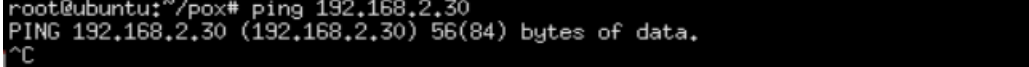
\includegraphics[width=0.7\linewidth]{files/CSE548_Fig_59-c1aa5b51d763c862731c6771e2933069.png}
\caption[]{Pings Blocked from Host 1 to Any Other Host}
\label{CSE548_Fig_59}
\end{figure}

\begin{figure}[!htbp]
\centering
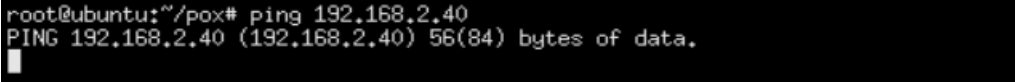
\includegraphics[width=0.7\linewidth]{files/CSE548_Fig_60-43d28c6559d13f0e2b94c535e9e67b9d.png}
\caption[]{Pings Blocked from Host 1 to Any Other Host}
\label{CSE548_Fig_60}
\end{figure}

We can see from Figure~\ref{CSE548_Fig_58}, Figure~\ref{CSE548_Fig_59}, and Figure~\ref{CSE548_Fig_60}: Pings Blocked from Host 1 to Any Other Host, that pings from Host 1 to any other Host are effectively blocked by the firewall.

\subparagraph{Project 4: Machine Learning-Based Anomaly Detection Project}

Once the machine learning models were trained, the learned weights and biases were saved in the Keras\footnote{Keras. \url{https://keras.io/}} format.  The saving of the trained models prevents having to go through the very time -- consuming training process during code development.  When saving the models, their training accuracy and loss histories were not preserved; therefore, their training accuracies and loss histories were saved as JSON files for later retrieval.  An example of the accuracy and loss history for Scenario A is shown in Figure~\ref{CSE548_Fig_61}: Scenario A Model Training Accuracy and Loss JSON File Contents below:

\begin{figure}[!htbp]
\centering
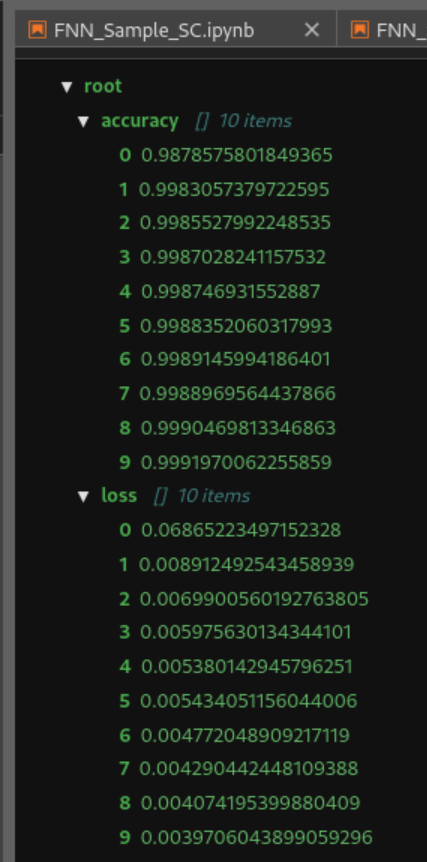
\includegraphics[width=0.7\linewidth]{files/CSE548_Fig_61-63a412639c85ae29a8ca2cbbd3ca9e4d.png}
\caption[]{Scenario A Model Training Accuracy and Loss JSON File Contents}
\label{CSE548_Fig_61}
\end{figure}

For Scenario A, the training accuracy and loss were then evaluated using the SKLearn \href{https://scikit-learn.org/stable/modules/generated/sklearn.metrics.accuracy\_score.html}{evaluate()} function.  The results of the evaluation are shown in Figure~\ref{CSE548_Fig_62}: Evaluate Training Accuracy and Loss:

\begin{figure}[!htbp]
\centering
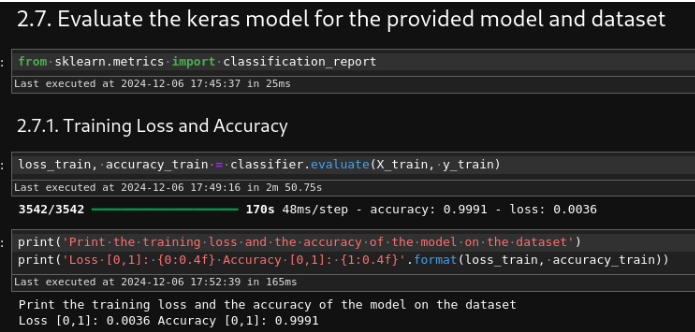
\includegraphics[width=0.7\linewidth]{files/CSE548_Fig_62-a2dbe046279a93ed65a6942c6dd04905.png}
\caption[]{Evaluate Training Accuracy and Loss}
\label{CSE548_Fig_62}
\end{figure}

We can see in Figure~\ref{CSE548_Fig_62}: Evaluate Training Accuracy and Loss, that the training accuracy is 0.9991 and the loss is 0.0036.  These are astonishingly great results, and may be an indication of overfitting.

We then evaluate the learned model on the testing dataset.  The results of this evaluation are shown in below:Figure~\ref{CSE548_Fig_63}: Evaluate Scenario A Test Accuracy and Loss:

\begin{figure}[!htbp]
\centering
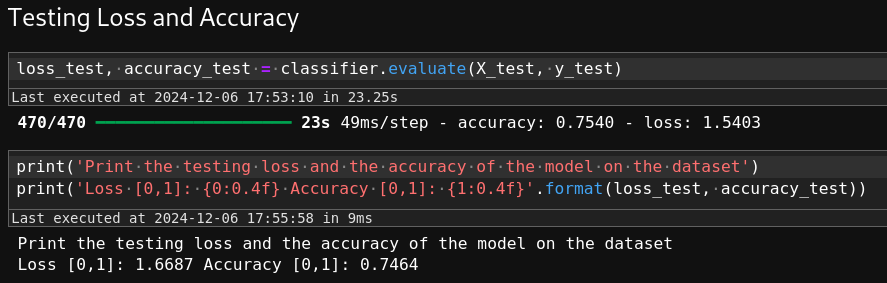
\includegraphics[width=0.7\linewidth]{files/CSE548_Fig_63-bfbb68c2886a07a2c754d96c8fe781ed.png}
\caption[]{Evaluate Scenario A Test Accuracy and Loss}
\label{CSE548_Fig_63}
\end{figure}

Although the testing accuracy in Figure~\ref{CSE548_Fig_63}: Evaluate Scenario A Test Accuracy and Loss, is lower and the loss is higher than for training, the model does pretty well against a testing dataset that does not contain data from the same classes and subclasses.

For Scenario B, the training and testing accuracy and loss are shown in Figure~\ref{CSE548_Fig_64}: Scenario B Training and Testing Accuracy and Loss below:

\begin{figure}[!htbp]
\centering
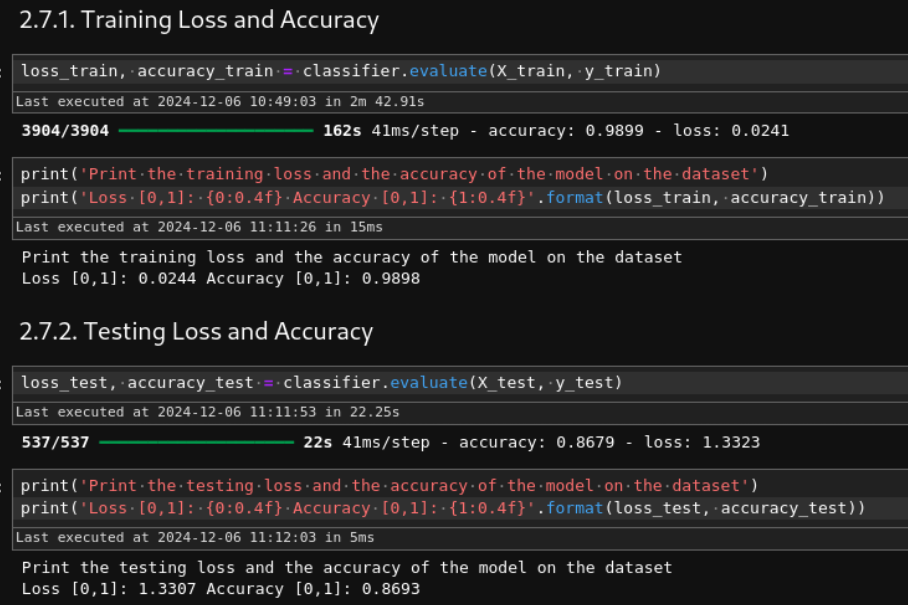
\includegraphics[width=0.7\linewidth]{files/CSE548_Fig_64-848a707661b8ec08685fcb1d7646bf98.png}
\caption[]{Scenario B Training and Testing Accuracy and Loss}
\label{CSE548_Fig_64}
\end{figure}

We can see from Figure~\ref{CSE548_Fig_64}: Scenario B Training and Testing Accuracy and Loss that although Scenario A has better training accuracy and lower training loss, Scenario B has better testing accuracy and lower testing loss.

For Scenario C, the training and testing accuracy and loss are shown in Figure~\ref{CSE548_Fig_65}: Scenario C Training and Testing Accuracy and Loss below:

\begin{figure}[!htbp]
\centering
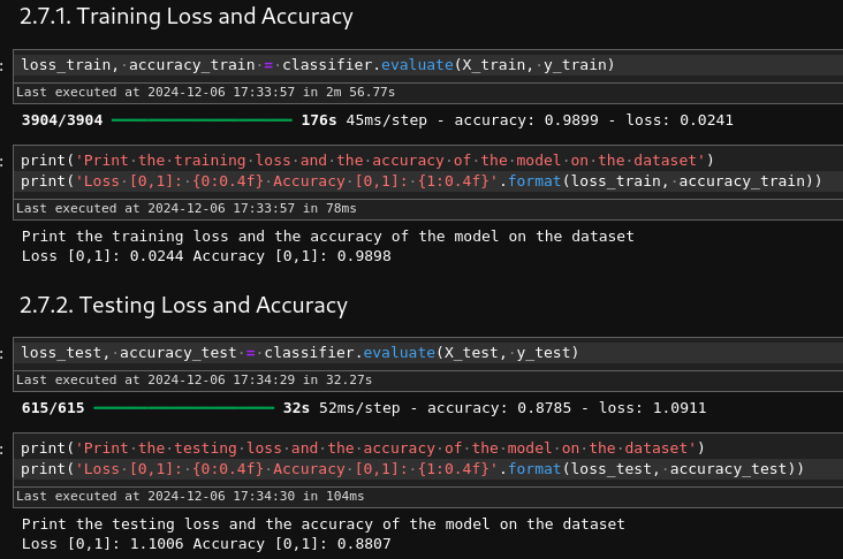
\includegraphics[width=0.7\linewidth]{files/CSE548_Fig_65-8721374381ca2f707d0162080070c1c0.png}
\caption[]{Scenario C Training and Testing Accuracy and Loss}
\label{CSE548_Fig_65}
\end{figure}

We can see from Figure~\ref{CSE548_Fig_65}: Scenario C Training and Testing Accuracy and Loss that Scenario C has lower training accuracy and training loss than scenario A, but it has better testing accuracy and lower testing loss than both scenario A and scenario B.

For Scenario A, we plot the training accuracy and loss as a function of training epoch.  The results are shown in Figure~\ref{CSE548_Fig_66}: Scenario A Model Training Accuracy and Figure~\ref{CSE548_Fig_67}: Scenario A Model Training Loss below:

\begin{figure}[!htbp]
\centering
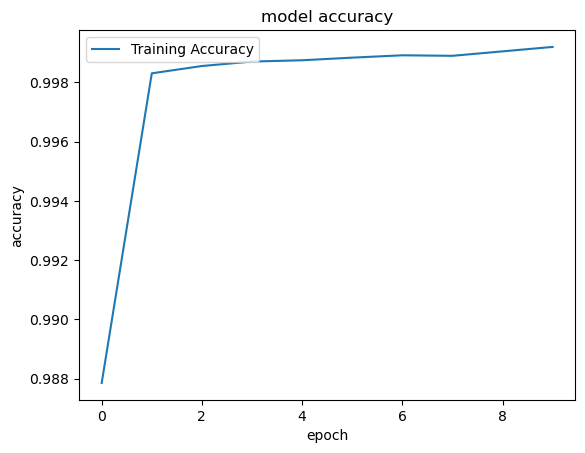
\includegraphics[width=0.7\linewidth]{files/CSE548_Fig_66-24e467a4d7e44d7be05d945df3ea6f6d.png}
\caption[]{Scenario A Model Training Accuracy}
\label{CSE548_Fig_66}
\end{figure}

\begin{figure}[!htbp]
\centering
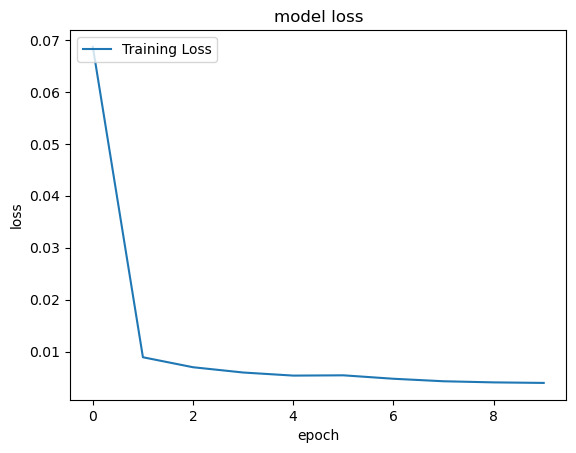
\includegraphics[width=0.7\linewidth]{files/CSE548_Fig_67-65a3a0480a3fd4930408809ea49e2f2d.png}
\caption[]{Scenario A Model Training Loss}
\label{CSE548_Fig_67}
\end{figure}

For Scenario B, we plot the training accuracy and loss in Figure~\ref{CSE548_Fig_68}: Scenario B Model Training Accuracy and Figure~\ref{CSE548_Fig_69}: Scenario B Model Training Loss below:

\begin{figure}[!htbp]
\centering
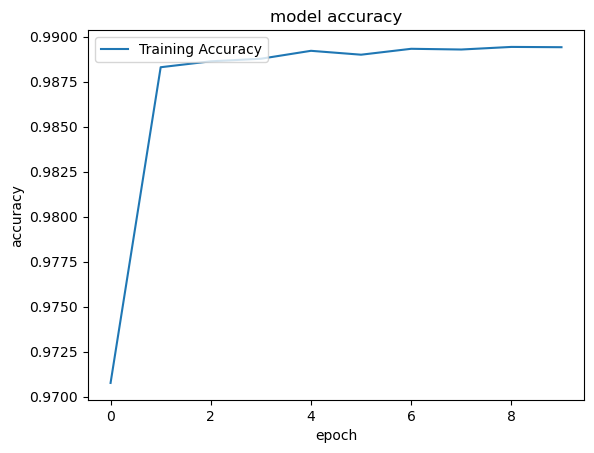
\includegraphics[width=0.7\linewidth]{files/CSE548_Fig_68-3f3a5b9be973f8889cc012e6a87f9db5.png}
\caption[]{Scenario B Model Training Accuracy}
\label{CSE548_Fig_68}
\end{figure}

\begin{figure}[!htbp]
\centering
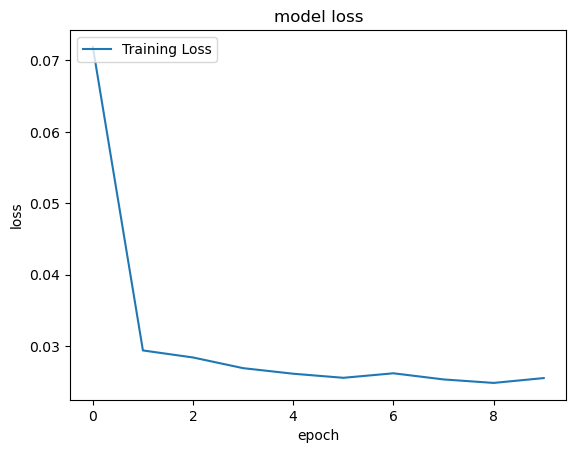
\includegraphics[width=0.7\linewidth]{files/CSE548_Fig_69-cf45b15738b852150355bc40e6286bed.png}
\caption[]{Scenario B Model Training Loss}
\label{CSE548_Fig_69}
\end{figure}

For Scenario C, we have the following model training accuracy and loss as shown in Figure~\ref{CSE548_Fig_70}: Scenario C Model Training Accuracy and Figure~\ref{CSE548_Fig_71}: Scenario C Model Training Loss.  We can see that Scenario B and Scenario C have the same training accuracy and training loss curves since both scenarios used the same model parameters and training data.

\begin{figure}[!htbp]
\centering
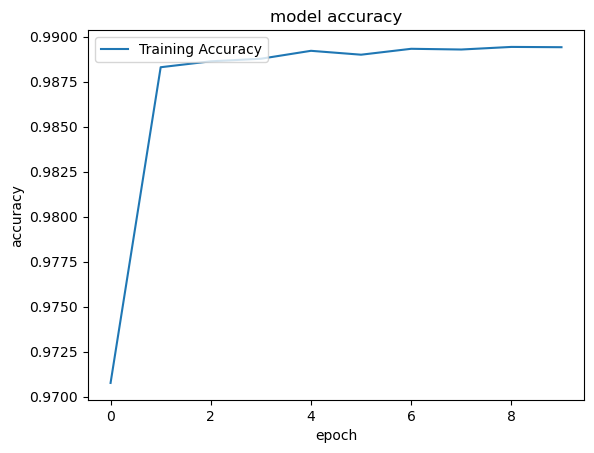
\includegraphics[width=0.7\linewidth]{files/CSE548_Fig_70-1b0e5121a319f85d07cc731f74b01d6a.png}
\caption[]{Scenario C Model Training Accuracy}
\label{CSE548_Fig_70}
\end{figure}

\begin{figure}[!htbp]
\centering
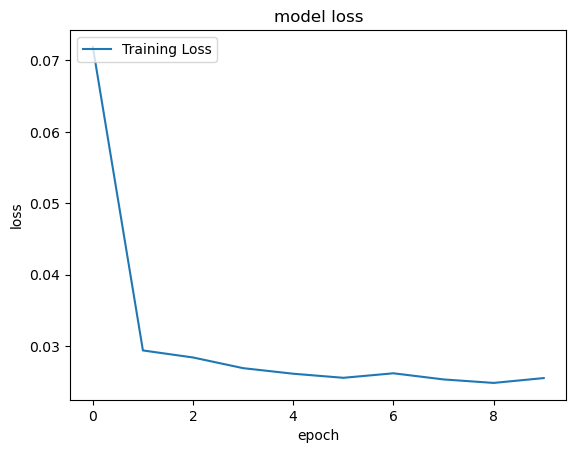
\includegraphics[width=0.7\linewidth]{files/CSE548_Fig_71-a50c5b3b2e319e952760b9c99d62aed6.png}
\caption[]{Scenario C Model Training Loss}
\label{CSE548_Fig_71}
\end{figure}

\subparagraph{Display Confusion Matrices and Scores}

We now show the confusion matrices and scores for each Scenario.  For Scenario A, we have the following confusion matrix, shown in Figure~\ref{CSE548_Fig_72}: Scenario A Confusion Matrix below:

\begin{figure}[!htbp]
\centering
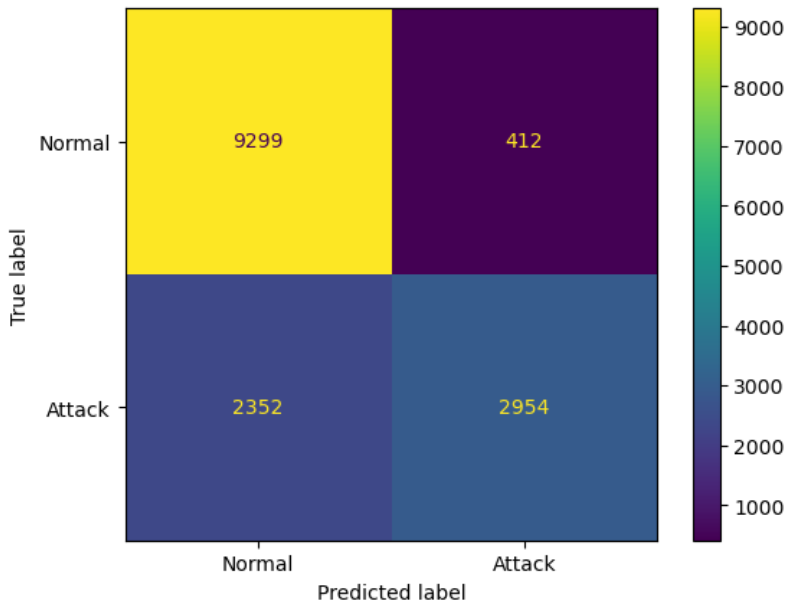
\includegraphics[width=0.7\linewidth]{files/CSE548_Fig_72-21961a39642cf140d7a4137c6ea688db.png}
\caption[]{Scenario A Confusion Matrix}
\label{CSE548_Fig_72}
\end{figure}

The confusion matrix in Figure~\ref{CSE548_Fig_72}: Scenario A Confusion Matrix indicates a large number of False Negatives (2352), which is not a good result for an attack detection model.

The model scores for Scenario A are shown in Figure~\ref{CSE548_Fig_73}: Scenario A Model Scores below:

\begin{figure}[!htbp]
\centering
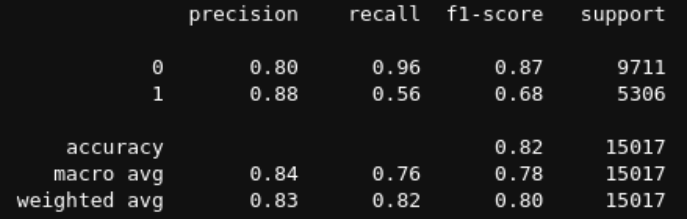
\includegraphics[width=0.7\linewidth]{files/CSE548_Fig_73-1d467ec9dad75fcd6c5922280de5576b.png}
\caption[]{Scenario A Model Scores}
\label{CSE548_Fig_73}
\end{figure}

As can be seen in Figure~\ref{CSE548_Fig_73}: Scenario A Model Scores, the precision is 0.8 for the Normal Class and 0.88 for the Attack Class.  This means that of all of the positive predictions, 0.8 of the predictions are correct for the Normal Class, and 0.88 are correct for the Attack Class.

However, when considering the Recall (i.e. True Positive Rate), we see that of all of the actual positives, the model correctly identified 0.96 of the Normal Classes, but only 0.56 of the Attack Classes.  Therefore, we can say that the model struggles to correctly predict when an attack is occuring.  This is somewhat not surprising since the model was tested on subclasses that it was not trained on.

For Scenario B, we have the following confusion matrix shown in Figure~\ref{CSE548_Fig_74}: Scenario B Confusion Matrix below:

\begin{figure}[!htbp]
\centering
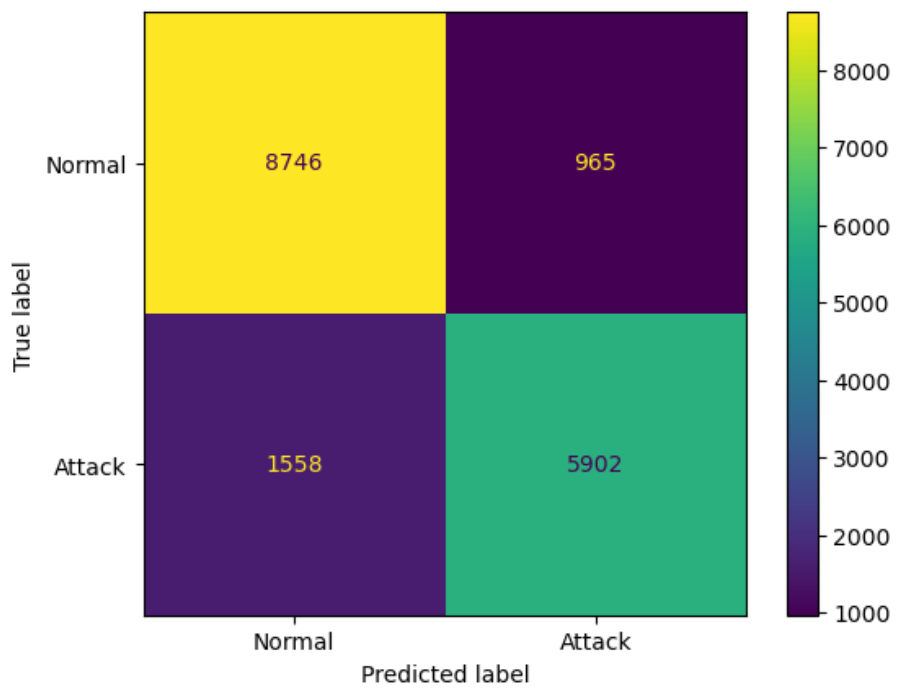
\includegraphics[width=0.7\linewidth]{files/CSE548_Fig_74-d5423714b6b60b2f9dc07a1b2a861eee.png}
\caption[]{Scenario B Confusion Matrix}
\label{CSE548_Fig_74}
\end{figure}

The confusion matrix shown in Figure~\ref{CSE548_Fig_74}: Scenario B Confusion Matrix indicates that Scenario B has a much lower amount of False Negatives (1558 vs 2352) than Scenario A.

The model scores for Scenario B are shown in Figure~\ref{CSE548_Fig_75}: Scenario B Model Scores below:

\begin{figure}[!htbp]
\centering
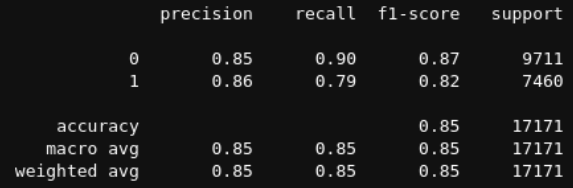
\includegraphics[width=0.7\linewidth]{files/CSE548_Fig_75-c2f4721e822ed9e246b99ceca336de13.png}
\caption[]{Scenario B Model Scores}
\label{CSE548_Fig_75}
\end{figure}

We observe from Figure~\ref{CSE548_Fig_75}: Scenario B Model Scores, the precision is 0.85 for the Normal Class and 0.86 for the Attack Class.  This means that of all of the positive predictions, 0.85 of the predictions are correct for the Normal Class, and 0.86 are correct for the Attack Class.  The precision of the Scenario A model are just slightly better than the Scenario B model; however, the Scenario B model has drastically better recall (i.e. true positive rate) performance.

We can see from Figure~\ref{CSE548_Fig_75}: Scenario B Model Scores, that the model for Scenario B had a recall (i.e. true positive rate) of 0.9 for the Normal Class and a recall (i.e. true positive rate) of 0.79 for the Attack Class.  The model in Scenario B performs much better in identifying actual attacks when compared to the model in Scenario A (recall of 0.79 vs recall of 0.56).

For Scenario C, we have the following confusion matrix shown in Figure~\ref{CSE548_Fig_76}: Scenario C Confusion Matrix below:

\begin{figure}[!htbp]
\centering
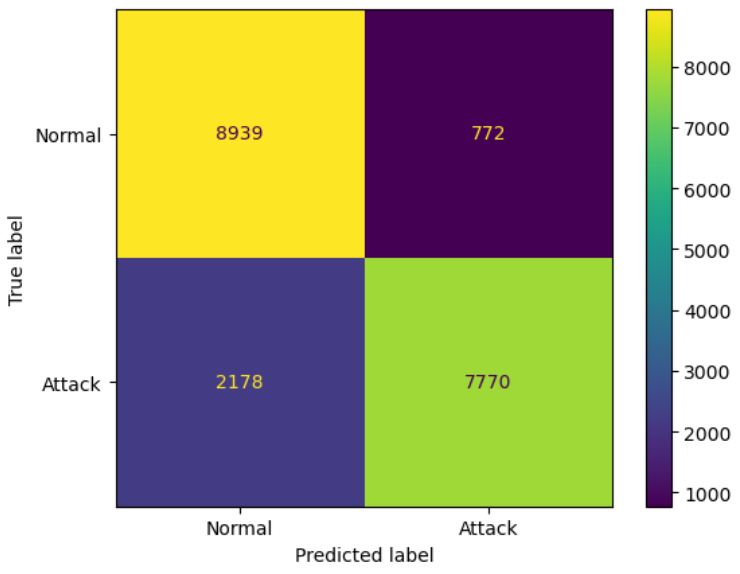
\includegraphics[width=0.7\linewidth]{files/CSE548_Fig_76-814329c099aa145556af03236cedbd58.png}
\caption[]{Scenario C Confusion Matrix}
\label{CSE548_Fig_76}
\end{figure}

The confusion matrix shown in Figure~\ref{CSE548_Fig_76}: Scenario C Confusion Matrix seems to indicate many False Negatives (2178); however, as a ratio to True Negatives (8939) and True Positives (7770), the model in this Scenario seems to perform better than the models in both Scenarios A and B.

The scores for the model in Scenario C are shown Figure~\ref{CSE548_Fig_77}: Scenario C Model Scores below:

\begin{figure}[!htbp]
\centering
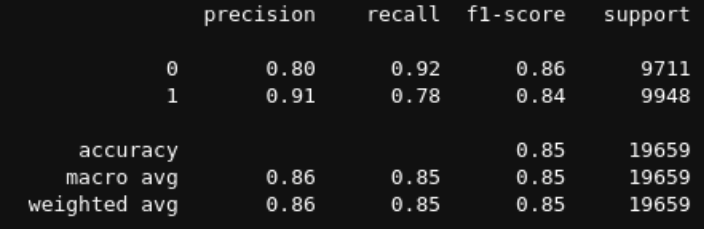
\includegraphics[width=0.7\linewidth]{files/CSE548_Fig_77-6adc31e7173ad2995b8ef9d142adfde6.png}
\caption[]{Scenario C Model Scores}
\label{CSE548_Fig_77}
\end{figure}

Observing the model score shown in Figure~\ref{CSE548_Fig_77}: Scenario C Model Scores, we see that the model in Scenario C has comparable precision (i.e. proportion of predicted positives that are correct) and recall (i.e. proportion of actual positives correctly identified) to the model in Scenario B, but has higher support (i.e. the number of actual occurrences of a class in the dataset) for those scores.  What is astonishing is that the model has such high precision and recall despite being tested on data that it has not been trained on (i.e. trained on subclasses A and B, tested on sublasses A, B and C).

It is observed that the model in Scenario A performed worse than the models in Scenario B and Scenario C when the testing subclasses differed from the training subclasses.  Astonishingly, even though scenario C was never training on attack subclass A3, it performed slightly better than scenario B.  Scenario B was trained on attack subclasses A1 and A2, but was tested on attack subclass A1.  Since it was already exposed to this attack subclass, it fared pretty well.  Scenario C was trained on attack subclasses A1 and A2, but not on A3.  Despite this, it still fared very well, even slightly better than scenario B.  This indicates that attack subclass A1 and A2 have some feature similarities to attack subclass C.

We can see from the bar charts in Figure~\ref{CSE548_Fig_22}: A1 and A3 Training Dataset Distribution of Attack Types and Figure~\ref{CSE548_Fig_24}: A2 and A4 Testing Dataset Distribution of Attack Types that for scenario A, there is no overlap in attack names.  The only commonality is the normal column.  Since the normal column magnitude is roughly an order of magnitude higher than the attacks, the model must be learning to recognize what is normal and using this to make a distinction.

For Scenario B, we can see from the bar charts in Figure~\ref{CSE548_Fig_23}: A1 and A2 Training Dataset Distribution of Attack Types and Figure~\ref{CSE548_Fig_25}: A1 Testing Dataset Distribution of Attack Types, that in addition to overlap on the normal class, there is significant overlap for the attack classes.

For Scenario C, we can see from the bar charts in Figure~\ref{CSE548_Fig_23}: A1 and A2 Training Dataset Distribution of Attack Types and Figure~\ref{CSE548_Fig_26}: A1, A2 and A3 Testing Dataset Distribution of Attack Types that in addition to significant normal class overlap, there is significant overlap in attack types, as well as additional attack types not seen in the training data.

We can get an even better idea of the performance of the model when observing the Receiver Operating Characteristic (ROC) Curve and Area Under the Curve (AUC).  For Scenario A, we have the following ROC and AUC shown in Figure~\ref{CSE548_Fig_78}: Scenario A Receiver Operating Characteristic Curve and Area Under the Curve below:

\begin{figure}[!htbp]
\centering
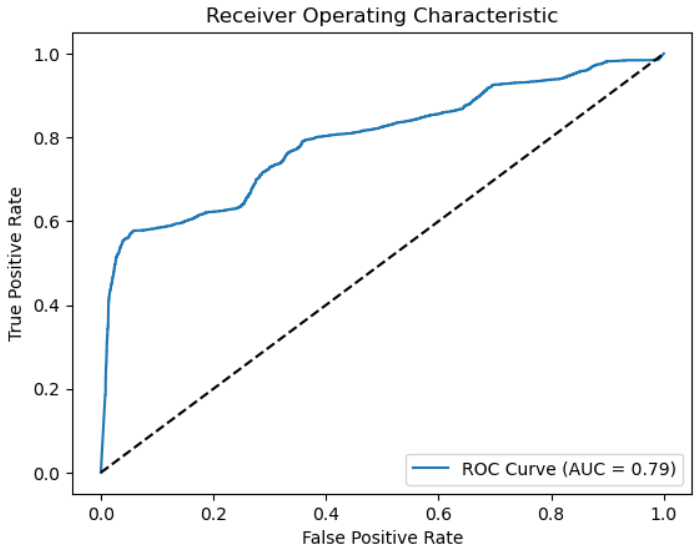
\includegraphics[width=0.7\linewidth]{files/CSE548_Fig_78-b0cbf38a5cc591a49b99e92a31348d9c.png}
\caption[]{Scenario A Receiver Operating Characteristic Curve and Area Under the Curve}
\label{CSE548_Fig_78}
\end{figure}

The ROC curve shown in Figure~\ref{CSE548_Fig_78}: Scenario A Receiver Operating Characteristic Curve and Area Under the Curve shows that it is difficult for this model to achieve a good True Positive Rate without starting to get unacceptably high False Positive rates.  The model is about 30 \% (i.e. 0.79 - 0.5) better than random guessing as indicated by the Area Under Curve\footnote{\href{https://en.wikipedia.org/wiki/Receiver\_operating\_characteristic}{Receiver operating characteristic}}.

For Scenario B, we have the ROC and AUC shown in Figure~\ref{CSE548_Fig_79}: Scenario B Receiver Operating Characteristic Curve and Area Under the Curve.  The ROC curve for Scenario B shows that this model is much better at achieving a high True Positive rate without a high False Positive rate.  The model is about 40\% (i.e. 0.89 - 0.5) better than random guessing as indicated by the Area Under Curve\footnote{\href{https://en.wikipedia.org/wiki/Receiver\_operating\_characteristic}{Receiver operating characteristic}}.

\begin{figure}[!htbp]
\centering
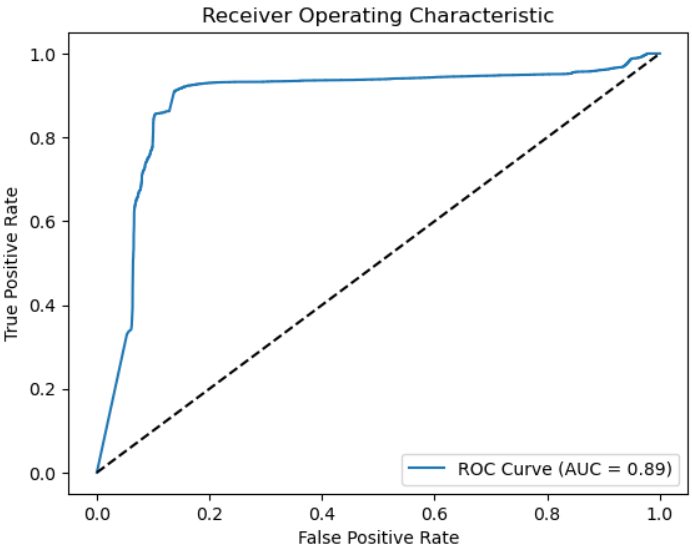
\includegraphics[width=0.7\linewidth]{files/CSE548_Fig_79-482c1c35a43f27532219a69a45367a93.png}
\caption[]{Scenario B Receiver Operating Characteristic Curve and Area Under the Curve}
\label{CSE548_Fig_79}
\end{figure}

For Scenario C, we have the ROC and AUC shown in Figure~\ref{CSE548_Fig_80}: Scenario C Receiver Operating Characteristic Curve and Area Under the Curve.  Scenario C has a ROC and AUC similar to scenario B.  This makes sense, since they were trained on the same dataset.  What is astonishing is that scenario C is tested on a wider variety of data but still performs slightly better than scenario B as seen from the AUC (0.9 for Scenario C vs 0.89 for Scenario B).  The conclusion is that there were enough similarities in the training and test data so that the model in Scenario C performed well.

\begin{figure}[!htbp]
\centering
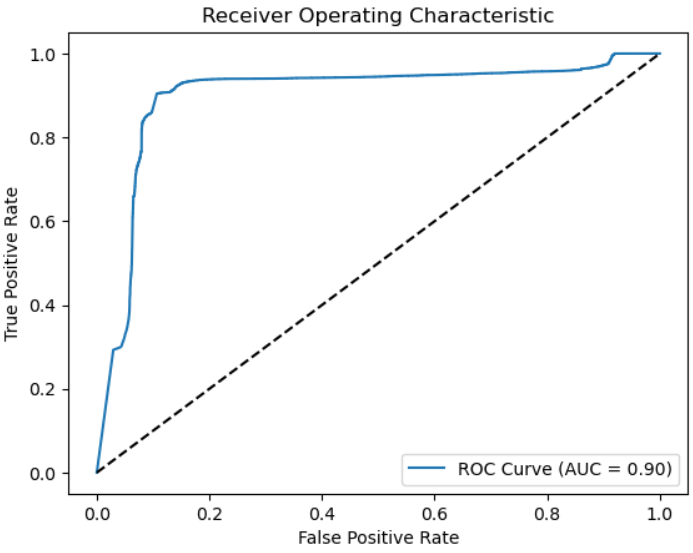
\includegraphics[width=0.7\linewidth]{files/CSE548_Fig_80-dc80e16c53efd22ff56cba74a2ef7cf3.png}
\caption[]{Scenario C Receiver Operating Characteristic Curve and Area Under the Curve}
\label{CSE548_Fig_80}
\end{figure}

\subparagraph{Description of my Contributions to the Project}

\subparagraph{Project 1: Packet Filter Firewall (iptables) Project}

For Project 1, I renamed the hostnames of the Virtual Machines (VMs) to `Client' and `Server' to enhance clarity of the report and prevent confusion as to which machine I am working with.  I figured out how to setup NAT networking on the two VMs so that they attached to the correct networks.

Additionally, it may not be apparent in the report, but working with \texttt{iptables}\footnote{\texttt{Iptables} is a user-space utility program that allows a system administrator to configure the IP packet filter rules of the Linux kernel firewall, implemented as different Netfilter modules. \href{https://netfilter.org/projects/iptables/index.html}{https://netfilter.org/projects/iptables/index.html}} and chains is very complicated.  I had to redo this section of the Project many times to get the operation that was required.  My selected method was to add one iptables rule at a time and test functionality.  If things operate as expected, then I add another rule.  If things break, I delete the rule and retest.  Sometimes, the rule sets get entangled and it is worth starting over.  I also learned about adding a default route to the Client.  This was necessary since the OS on the Client would not know what to do with packets whose destination IP address is outside of the attached network.
I have been working with web server for many years, so I knew how to quickly setup an Apache webserver on the Gateway/Server, even though the Python simple webserver would have been sufficient.  I also used the \texttt{curl}\footnote{\texttt{curl} is a command-line tool for transferring data specified with URL syntax. \href{https://curl.se/docs/manpage.html}{https://curl.se/docs/manpage.html}} command to rapidly test whether the web server was working.

\subparagraph{Project 2: SDN-Based Stateless Firewall Project}

In Project 2, I used the Linux \texttt{Terminator}\footnote{\texttt{Terminator} is a terminal emulator for Linux which allows users to arrange multiple terminal windows in a grid. \href{https://terminator-gtk3.readthedocs.io/en/latest/}{https://terminator-gtk3.readthedocs.io/en/latest/}} terminal application to subdivide the terminal window into quadrants, so I can view the OpenFlow switch status, the POX controller status and the OpenFlow Switch's traffic flows.  This greatly enhanced understanding of the operation of the components in real time.

\subparagraph{Project 3: SDN-Based DoS Attacks and Mitigation Project}

In Project 3, in order to see the DoS attack happening in real time, I used the \texttt{iptraf-ng}[myref\_12] application to watch packet counters of packets on the network.  It was readily apparent that a packet flood was occurring since almost 4 million packets were sent by the offending Host, and the data rate was over 45 megabits/second.

In the code writing process for the \href{/sections/mcs-projects/mcs-portfolio-project/l3firewall}{\texttt{L3Firewall.py}} application, I placed many debug output points that helped to figure out whether the code was operating as intended.

\subparagraph{Project 4: Machine Learning-Based Anomaly Detection Project}

In Project 4, I converted the provided Python scripts into \texttt{IPython}\footnote{IPython. \href{https://ipython.org/}{https://ipython.org/}} Notebooks in the \texttt{Jupyter Lab}\footnote{\texttt{JupyterLab} is an open-source web-based interactive development environment for Jupyter notebooks, code, and data. \href{https://jupyter.org/}{https://jupyter.org/}} environment.  I broke down the provided scripts into code cells according to logical divisions and made enhancements such as debug points as necessary.  This enabled understanding of exactly what the scripts were supposed to do.  I also added the ability to save the trained models into \texttt{Keras}\footnote{Keras. \url{https://keras.io/}} files, and the training accuracy and loss history into \texttt{JSON}\footnote{\texttt{JSON} (JavaScript Object Notation) is a lightweight data-interchange format that is easy for humans to read and write, and easy for machines to parse and generate. \href{https://www.json.org/json-en.html}{https://www.json.org/json-en.html}} files.  This enabled development of the code without having to wait an extremely long time to retrain the models.

\subparagraph{Explanation of New Skills, Techniques, or Knowledge Acquired from the Project}

\subparagraph{Project 1: Packet Filter Firewall (iptables) Project}

A lesson that I learned was that it was worth taking the time to enter the \texttt{iptables}\footnote{\texttt{Iptables} is a user-space utility program that allows a system administrator to configure the IP packet filter rules of the Linux kernel firewall, implemented as different Netfilter modules. \href{https://netfilter.org/projects/iptables/index.html}{https://netfilter.org/projects/iptables/index.html}} commands one at a time and checking the iptables chains using:

\begin{verbatim}
iptables -L
\end{verbatim}

I also learned how to fix errors by using the \texttt{--line-numbers} switch and the \texttt{-D} switch to delete mistakes.  \texttt{Iptables}\footnote{\texttt{Iptables} is a user-space utility program that allows a system administrator to configure the IP packet filter rules of the Linux kernel firewall, implemented as different Netfilter modules. \href{https://netfilter.org/projects/iptables/index.html}{https://netfilter.org/projects/iptables/index.html}} chains can become complicated, so it is worth to flush the entire chains and start over when things stop working.  I also learned that the \texttt{-A} switch will append a rule to the end, while the \texttt{-I} switch will insert a rule to the top.  The order of the rules matters, so that if there is a \texttt{DROP} before an \texttt{ACCEPT}, then the packet will be dropped.

\subparagraph{Project 2: SDN-Based Stateless Firewall Project}

An Open Virtual Switch[\^mref\_1] was set up and four containers were connected to it.  Firewall rules were set into place to provide security as per Project requirements.  The firewall was tested against various test conditions.  After performing the labs, the project was pretty straightforward.  I did learn about \texttt{hping}\footnote{\texttt{hping} is a command-line oriented TCP/IP packet assembler/analyzer. The interface is inspired to the ping(8) Unix command, but hping isn't only able to send ICMP echo requests. It supports TCP, UDP, ICMP and RAW-IP protocols, has a traceroute mode, the ability to send files between a covered channel, and many other features. \href{https://en.wikipedia.org/wiki/Hping}{Hping}, \href{https://www.hping.org/wiki-sub/index/}{https://www.hping.org/wiki-sub/index/}}, which is a very powerful alternative to the standard Linux \texttt{ping}\footnote{\texttt{ping} is a computer network administration utility used to test the reachability of a host on an Internet Protocol (IP) network. It measures the round-trip time for messages sent from the originating host to a destination computer that are echoed back to the source. \href{https://en.wikipedia.org/wiki/Ping\_(networking\_utility)}{Ping (networking utility)}} command.

One thing that I did notice is that the firewall would stop working after a certain time.  After restarting the POX process, the firewall would work correctly.  I am not sure if this is a bug or proper behavior.  The network traffic that was examined with \texttt{Wireshark}\footnote{\texttt{Wireshark} is a free and open-source packet analyzer. It is used for network troubleshooting, analysis, software and communications protocol development, and education. \href{https://www.wireshark.org/}{https://www.wireshark.org/}} did not exhibit any anomalous behavior that precipitated the firewall shutting down.

\subparagraph{Project 3: SDN-Based DoS Attacks and Mitigation Project}

An Open Virtual Switch was set up and 4 containers were connected to it.  A DoS attack was performed that indicated that the baseline firewall configuration was susceptible to such attacks.  The \href{/sections/mcs-projects/mcs-portfolio-project/l3firewall}{\texttt{L3Firewall.py}} application was modified to detect and permanently block the offending host by \texttt{MAC}\footnote{A \texttt{Media Access Control address (MAC address)} is a unique identifier assigned to a network interface controller (NIC) for use as a network address in communications within a network segment. \href{https://en.wikipedia.org/wiki/MAC\_address}{MAC address}} address.  Successful operation of the DoS mitigation was demonstrated.

I learned much about how the \texttt{Open Virtual Switch}\footnote{OpenFlow Switch Specification. \href{https://opennetworking.org/}{https://opennetworking.org/}} operates and deals with traffic flows by observing the addition of flow rules to the learning firewall.  When modifying the \href{/sections/mcs-projects/mcs-portfolio-project/l3firewall}{\texttt{L3Firewall.py}} application, I learned about the format of the procedural calls and functions within the \texttt{Open Virtual Switch}\footnote{OpenFlow Switch Specification. \href{https://opennetworking.org/}{https://opennetworking.org/}} framework that examines flows and packets.  These procedural calls and functions can then be used to block traffic that matches the criteria of a DoS style attack.

\subparagraph{Project 4: Machine Learning-Based Anomaly Detection Project}

In Project 4, we were provided with lots of Python code to get started.  My favorite method of performing Data Science is to use \texttt{IPython Notebooks}\footnote{IPython. \href{https://ipython.org/}{https://ipython.org/}} in the \texttt{Jupyter Lab}\footnote{\texttt{JupyterLab} is an open-source web-based interactive development environment for Jupyter notebooks, code, and data. \href{https://jupyter.org/}{https://jupyter.org/}} environment.  I used the provided \href{/sections/mcs-projects/mcs-portfolio-project/dataextractor}{\texttt{dataExtractor.py}} to create a \texttt{IPython Notebook}\footnote{IPython. \href{https://ipython.org/}{https://ipython.org/}} based on this script to create the training subclass datasets.  Data label and preprocessing methods were taken out of the provided data\_preprocessor.py and distinctLabelExtractor.py scripts and incorporated into more general Notebooks called \href{/sections/mcs-projects/mcs-portfolio-project/fnn-sample-sa}{FNN Sample SA}, \href{/sections/mcs-projects/mcs-portfolio-project/fnn-sample-sb}{FNN Sample SB}, \href{/sections/mcs-projects/mcs-portfolio-project/fnn-sample-sc}{FNN Sample SC}.  It was decided to use three separate Notebooks to faciliate code reuse without having to rename general variable names.
Since the model training takes a very long time, I learned how to save the trained model into a \texttt{Keras}\footnote{Keras. \url{https://keras.io/}} file, as well as saving the training accuracy and loss histories into \texttt{JSON}\footnote{\texttt{JSON} (JavaScript Object Notation) is a lightweight data-interchange format that is easy for humans to read and write, and easy for machines to parse and generate. \href{https://www.json.org/json-en.html}{https://www.json.org/json-en.html}} files for later recall.  At first glance, it was not trivial to identify the best performing model, since the model in Scenario A had such a high training accuracy.  Therefore, I had to learn to investigate the precision, recall, ROC and AUC characteristics of each model to get a better feel for which model peformed the best.

\paragraph{CSE572 Data Mining: Portfolio Project Report}

\textbf{Abstract} --- Insulin Pump and Continuous Glucose Monitor sensor data were analyzed from three different vantage points in this study.  The first analysis resulted in an understanding of the amount time a patient dwells in a blood glucose classification level.  The second study looked at whether certain extracted features could be used to train a Support Vector Machine to classify whether a patient has eaten a meal or not.  Remarkably, the accuracy of the learned model was \textgreater  99\%.  Finally, clustering was performed on the extracted features and compared to ground truth.

\subparagraph{1. Introduction and Problem Statement}

In this portfolio project report, we will be reviewing the results obtained from the three projects in this course.  The first project consisted of extracting glucose level time series data and its properties for a person using an artificial pancreas.  The second project consisted of training a machine model to assess whether the person has eaten a meal or not.  While the third project consisted of clustering the glucose data to determine the amount of carbohydrates the person has consumed in each meal.

The artificial pancreas used by the person is the Medtronic 670G\footnote{Medtronic 670G Hybrid Closed Loop System. \href{https://www.medtronicdiabetes.com/products/minimed-670g-insulin-pump-system}{https://www.medtronicdiabetes.com/products/minimed-670g-insulin-pump-system}} control system.  The system consists of a continuous glucose monitor (CGM), which is used to collect blood glucose measurements every five minutes.  Based on these readings a feedback control system delivers precise amounts of insulin to the person.  We will be analyzing the Insulin Pump and CGM Sensor data for the projects and this report.

\subparagraph{Explanation of the Solution}

\subparagraph{Project 1: Extracting Time Series Properties of Glucose Levels in Artificial Pancreas Project}

Data for this project was provided as two separated Comma Separated Value (CSV) files.  The first CSV file contained CGM sensor data, while the second contained insuling pump data.  Both the CGM sensor data and insulin pump data were in reversed chronological order, meaning the latest data were the first rows of the files.  Additionally, the data from the CGM sensor and insulin pump were taken asynchronously from each other; therefore, synchronization would have to be performed.  The CGM sensor and insulin pump data also had many columns that added unecessary dimensionality that needed to be reduced.  Finally, there were many missing data points and over fifty -- five thousand rows of data.  An effective strategy was required for dealing with the missing data points and the sheer number of rows.

The data for both the insulin pump and the CGM sensor were loaded into Pandas\footnote{Pandas. \href{https://pandas.pydata.org/}{https://pandas.pydata.org/}} dataframes.  In order to perform Exploratory Data Analysis (EDA) and plotting of the CGM sensor data, the data was reversed into proper chronological order and filtered to only include the date and time, Sensor Glucose reading in mg/dL, and raw sensor (ISIG) value columns.  The insulin pump data was reversed into proper chronological order and filtered to only include the date and time, and the alarm mode column.

To effectively synchronize the CGM sensor and insulin pump data, a \textit{``datetime''} column was added to each dataset using the \texttt{datatime()}\footnote{The \texttt{datetime} module supplies classes for manipulating dates and times in both simple and complex ways. While date and time arithmetic is supported, the focus of the implementation is on efficient attribute extraction for output formatting and manipulation. \href{https://docs.python.org/3/library/datetime.html}{https://docs.python.org/3/library/datetime.html}} method in the Pandas Python module.  The \textit{``datetime''} column is a concatenation of the date and time columns within the datasets.

The project required knowledge of when the insulin pump was set to Auto Mode.  A reading of ``AUTO MODE ACTIVE PLGM OFF'' in the Alarm column of the insulin pump dataset indicates the start of the date and time for when Auto Mode is activated.  Once in Auto Mode, the insulin pump can not go back to manual mode without a reset.  With the datasets both having a datetime column, a search can be made from when the insulin pump was set to Auto Mode.  The corresponding data point with the closest time stamp in the CGM sensor dataset was then found.  A ``Sensor Mode'' column was added CGM sensor dataframe and each row was then assigned whether it is data from Manual Mode or Auto Mode.

To find the daily averages, it is necessary to know the number of data points per day.  Since each data point corresponds to a 5 minute increment, simple arithmetic provides that there are 288 data points per 24 hour period.  Note that this number may include missing data points.  To find the overall averages required for the project, day numbers were added to the CGM dataframe.  Day numbers were simply derived as 24 -- hour periods from the datetime column.  The maximum day number can then be used to calculate the overall averages that were required in this project.  The number of days of data per this methodology turned out to be 203.  The rows were then characterized as either day time or overnight by looking at the hour in the datetime column and assigning 6AM to 12AM as ``daytime'' and 12AM to 6AM as ``overnight''.

Handling missing data is an extremely critical part of data cleaning and preparation.  For this stage of the Project, the Pandas' linear interpolation method was used on the CGM Sensor Glucose column without further consideration for correctness;  with the assumption being that glucose levels should follow an orderly change from a last known reading.

Lastly, classification of glucose levels was required by the project as shown in Table~\ref{CSE572_Table_1}: Glucose Classification Levels.

\begin{table}
\centering
\caption[]{Glucose Classification Levels}
\label{CSE572_Table_1}
\begin{tabular}{p{\dimexpr 0.500\linewidth-2\tabcolsep}p{\dimexpr 0.500\linewidth-2\tabcolsep}}
\toprule
Glucose Level [mg/dL] & Classification Level \\
\hline
level \textgreater  250 & Hyperglycemia Critical \\
level \textgreater  180 & Hyperglycemia \\
70 \textless = level \textless = 180 & Normal \\
70 \textless = level \textless = 150 & Secondary \\
54 \textless  level \textless  70 & Hypoglycemia Level 1 \\
level \textless = 54 & Hypoglycemia Level 2 \\
\bottomrule
\end{tabular}
\end{table}

Now that the dataframes were cleaned and prepared, calculations of daily and overall means for the various categories could be performed.  The project required calculation of means for 18 different categories.  This number is arrived by realizing that there are 6 classification levels given in Table~\ref{CSE572_Table_1}: Glucose Classification Levels, and each classification level is to be averaged over the overnight, day time and whole day time periods.  Additionally, these 18 categories are to be evaluated for both when the insulin pump is in Manual Mode or Auto Mode, for a total of 36 separate mean calculations.

An example of a mean calculation would be to select from the overall data the appropriate categorical conditions, group that data by day and count the number of data items.  This effectively gives the amount of time the person's blood glucose levels were in a specific range category per day.  A per day mean and a mean for the entire dataset can then be calculated.

\subparagraph{Project 2: Machine Model Training Project}

The goal of this project is to train a machine to differentiate between the person eating a meal versus not eating a meal given the person's CGM sensor's time series data.  As in Project 1, insulin pump and CGM sensor data were provided; however, for this project two sets of data were available.

The datasets had similar problems that occurred in Project 1; however, Project 2's insulin pump datasets had the additional issue of non -- uniform date and time recording.  This necessitated an additional step of pre -- processing of the date and time columns within the datasets.  As in Project 1, the now cleaned date and time columns were combined into a ``datetime'' column using the \texttt{to\_datetime()}\footnote{The \texttt{to\_datetime()} function in the Pandas Python module is used to convert a string or a list of strings to datetime objects. \href{https://pandas.pydata.org/pandas-docs/stable/reference/api/pandas.to\_datetime.html}{https://pandas.pydata.org/pandas-docs/stable/reference/api/pandas.to\_datetime.html}} method provided by the Pandas Python module.

To train a machine learning model, rows from the datasets had to be extracted that corresponded to the person eating a meal.  It was assumed that an occurrence of a non -- NaN and positive entry in the ``BWZ Carb Input (grams)'' column corresponds to the start of a meal.  The time stamps for each of these rows were saved into a sub -- dataframe for further processing.

A meal window was defined as a 2 hour time period from when there is an entry in the meal start time sub -- dataframe.  If that window was empty, then the corresponding CGM sensor data for time period of meal time -- 30 minute to meal time + 2 hours was added to a separate agglomerated dataset.  The adding of meal data to the separate agglomerated dataset was somewhat complicated by the fact that meals might occur within the 2 hour meal window.  In that case the meal occurs within the window is ignored.  If a meal occurs exactly at the end of the 2 hour window, then data from meal time -- 1 hour and meal time + 4 hours is used.

Since the CGM sensor provides data at 5 minute intervals, a time period of 2.5 hours results in 30 CGM sensor data points.  Sometimes, due to missing data from the CGM sensor, less than 30 data points are available.  It was decided to drop any rows that contained less than 30 data points, as there was sufficient data available to train the machine.  The separate agglomerated CGM sensor readings data were then converted into a Numpy\footnote{\texttt{NumPy} is a library for the Python programming language, adding support for large, multi-dimensional arrays and matrices, along with a large collection of high-level mathematical functions to operate on these arrays. \url{https://numpy.org/}} matrix to facilitate use of Sklearn's[myref\_8] machine learning Python Modules.

For the no -- meal data, a similar procedure was followed except that the post -- absorbtive window was defined as a meal time + 2 hours to meal time + 4 hours.  If there were any meals in this post -- absorbtive period, then data for that period was ignored.  However, if the post -- absorbtive window had any 0 or NaN data points, the 0's or NaN's were ignored and data for that post -- absorbtive stretch was added into the agglomerated sub -- datasets.

Since the post -- absorbtive window is 2 hours, CGM sensor data at 5 minute interval results in 24 data points.  Any rows that had less than 24 data points were dropped since there was sufficient data to train the machine.
Even though rows with less than 30 data points in the meal data and rows with less than 24 data points in the no -- meal data were excluded, the intra -- row data might still contain NaN's.

It was decided to use \href{https://grokipedia.com/page/Imputation\_(statistics)}{imputation} to handle these missing data points.  The problem is that if the amount of missing data points is too high, then imputation would provide erroneous results.  A heuristic threshold of 10\% missing data points was chosen as a drop threshold.  From the rows that were left, the missing data points were handled with Sklearn's\footnote{Scikit-learn. \href{https://scikit-learn.org/}{https://scikit-learn.org/}} KNN (K -- Nearest Neighbor) Imputer\footnote{The \texttt{KNNImputer} class in the Sklearn Python module provides imputation for completing missing values using the k-Nearest Neighbors approach. \href{https://scikit-learn.org/stable/modules/generated/sklearn.impute.KNNImputer.html}{https://scikit-learn.org/stable/modules/generated/sklearn.impute.KNNImputer.html}}.  The K used for the KNN Imputer was 7.  This value was chosen based on a heuristic estimate.

\begin{framed}
\textbf{Additional Context from Copilot}\\
K in KNN (k‑Nearest Neighbors)

\begin{itemize}
\item K = number of nearest training instances used to make a prediction.
\item Classification: predicted class = majority vote among the K nearest neighbors (ties often broken by using odd K or tie‑breaker rule).
\item Regression: predicted value = average (or distance‑weighted average) of the K neighbors' values.
\item Effect:

\begin{itemize}
\item small K \rightarrow low bias, high variance (sensitive to noise, more overfitting)
\item large K \rightarrow high bias, low variance (smoother decision boundary, may underfit)
\end{itemize}


\item Choosing K: use cross‑validation; ensure K $\leq$ number of training samples; common practice uses odd K for binary classification.
\end{itemize}
\end{framed}

Now that the meal and no -- meal datasets were cleaned and imputed, features can be extracted that are used to train the machine learning model.  The eight features that were selected were:

\begin{itemize}
\item Mean for the row
\item Standard deviation for the row
\item Maximum value for the row
\item Minimum value for the row
\item Mean first derivative for the row
\item Mean second derivative for the row
\item Area of the curve (AUC) for the row
\item Time to reach the peak for the row
\end{itemize}

These features were then extracted for each row using a feature extractor function.

Since it is known which data corresponds to a meal or not, class labels were then added to the meal data and no -- meal data feature matrices.  A class label of 1 was added to the meal data feature matrix and a class label of 0 was added to the no -- meal feature matrix.  The meal and no meal feature matrices were then vertically stacked using Numpy's\footnote{\texttt{NumPy} is a library for the Python programming language, adding support for large, multi-dimensional arrays and matrices, along with a large collection of high-level mathematical functions to operate on these arrays. \url{https://numpy.org/}} \texttt{vstack}\footnote{The \texttt{vstack()} function in the Numpy Python module is used to stack arrays in sequence vertically (row wise). \href{https://numpy.org/doc/stable/reference/generated/numpy.vstack.html}{https://numpy.org/doc/stable/reference/generated/numpy.vstack.html}} method.  The training data was then sliced off and labeled as ``X'', while the class labels were sliced off and labeled as ``y'' following machine learning conventions.

Sklearn's\footnote{Scikit-learn. \href{https://scikit-learn.org/}{https://scikit-learn.org/}} \texttt{train\_test\_split}\footnote{The \texttt{train\_test\_split()} function in the Sklearn Python module is used to split arrays or matrices into random train and test subsets. \href{https://scikit-learn.org/stable/modules/generated/sklearn.model\_selection.train\_test\_split.html}{https://scikit-learn.org/stable/modules/generated/sklearn.model\_selection.train\_test\_split.html}} was then used to split the data into a training sub -- dataset and a testing sub -- dataset with a 80\% / 20\% ratio, respectively.  The training and testing datasets were then normalized using Sklearn's\footnote{Scikit-learn. \href{https://scikit-learn.org/}{https://scikit-learn.org/}} \texttt{StandardScaler}\footnote{The StandardScaler class in the Sklearn Python module is used to standardize features by removing the mean and scaling to unit variance. \href{https://scikit-learn.org/stable/modules/generated/sklearn.preprocessing.StandardScaler.html}{https://scikit-learn.org/stable/modules/generated/sklearn.preprocessing.StandardScaler.html}} class.

For this Project, it was decided to employ a \texttt{Support Vector Machine (SVM)}\footnote{A \texttt{Support Vector Machine (SVM)} is a supervised machine learning model that uses classification algorithms for two-group classification problems. After giving an SVM model sets of labeled training data for each category, they're able to categorize new text. \href{https://en.wikipedia.org/wiki/Support\_vector\_machine}{Support vector machine}} machine learning model, although a \texttt{Decision Tree}\footnote{\texttt{Decision Tree} learning is a supervised learning approach used in statistics, data mining and machine learning. In this formalism, a classification or regression decision tree is used as a predictive model to draw conclusions about a set of observations. \href{https://en.wikipedia.org/wiki/Decision\_tree\_learning}{Decision tree learning}} machine learning model would have also been a good choice for this binary classification problem.  A linear kernel was chosen since the dimensionality of eight is rather high, but the features have linearly seperable charactersitics.  To prevent overfitting (low bias, high variance), a Regularization Parameter (C) of 0.1 was chosen.

\begin{framed}
\textbf{Additional Context from Copilot}\\
SVM kernels and the regularization parameter C --- concise guide

\begin{itemize}
\item Kernel concept

\begin{itemize}
\item Kernel k(x,y)=⟨$\varphi$(x),$\varphi$(y)⟩ lets SVM operate in a transformed feature space without explicit mapping (kernel trick). Choose based on assumed decision-boundary shape.
\end{itemize}


\item Common kernels (form + when to use)

\begin{itemize}
\item Linear: k(x,y)=x·y

\begin{itemize}
\item Use when data is (nearly) linearly separable or \#features ≫ \#samples; fast and interpretable.
\end{itemize}


\item Polynomial: k(x,y)=($\gamma$ x·y + coef0)\^degree

\begin{itemize}
\item Captures feature interactions; degree controls complexity (degree=2 or 3 typical). Can overfit at high degree.
\end{itemize}


\item RBF / Gaussian: k(x,y)=exp(-$\gamma$ ||x-y||\^2)

\begin{itemize}
\item Default choice for many problems. $\gamma$ controls influence radius: small $\gamma$ \rightarrow smooth boundary (underfit); large $\gamma$ \rightarrow localized, complex boundary (overfit).
\end{itemize}


\item Sigmoid: k(x,y)=tanh($\gamma$ x·y + coef0)

\begin{itemize}
\item Behaves like a two‑layer neural net; less commonly used and may not satisfy Mercer conditions for all params.
\end{itemize}


\item Custom kernels: allowed but must be positive semi‑definite (Mercer) for SVM guarantees.
\end{itemize}


\item Kernel hyperparameters to tune

\begin{itemize}
\item \texttt{degree} (polynomial), \texttt{gamma} (RBF/poly/sigmoid), \texttt{coef0} (poly/sigmoid). Defaults (e.g., \texttt{gamma='scale'}) are common but cross‑validate.
\end{itemize}


\item Regularization parameter C (intuition + effect)

\begin{itemize}
\item SVM objective (soft‑margin): minimize 1/2 ||w||\^2 + C $\Sigma$ $\xi$\_i  subject to margin constraints.
\item C controls trade‑off between margin width and training errors:

\begin{itemize}
\item Large C \rightarrow penalize slack heavily \rightarrow narrower margin, fewer training errors (low bias, higher variance / potential overfit).
\item Small C \rightarrow allow more slack \rightarrow wider margin, more regularization (higher bias, lower variance / potential underfit).
\end{itemize}


\item Practical rule: grid‑search C on log scale (e.g., 1e-3 \dots 1e3).
\end{itemize}


\item Practical tips

\begin{itemize}
\item Always scale/normalize features before kernel SVM.
\item If data is high‑dimensional and linear performance is acceptable, use linear SVM for speed (or LinearSVC).
\item Start with RBF + CV over \{C, $\gamma$\}; if that fails, try polynomial or custom kernels informed by domain knowledge.
\end{itemize}
\end{itemize}
\end{framed}

The SVM model was then trained on the normalized training data and an accuracy of 99.71\% was the result.  Additionally, the F1 score was calculated to be 1.00.

\begin{framed}
\textbf{Additional Context from Copilot}\\
F1 score = harmonic mean of precision and recall:

\begin{itemize}
\item Formula:

\begin{equation}
F_1 = 2\cdot\frac{\text{precision}\cdot\text{recall}}{\text{precision}+\text{recall}}
\end{equation}


\item Precision:

\begin{equation}
\text{precision} = \frac{TP}{TP + FP}
\end{equation}


\item Recall:

\begin{equation}
\text{recall} = \frac{TP}{TP + FN}
\end{equation}


\item Purpose: balances precision and recall into a single metric (better than arithmetic mean when values differ).
\item Range: 0--1 (higher is better). Use when you need a single measure that penalizes extreme imbalance between precision and recall.
\end{itemize}

What the extremes mean:

\begin{itemize}
\item F1 = 0: occurs when \texttt{TP = 0} (so precision = 0 and/or recall = 0). The model makes no correct positive predictions or misses all positives.
\item F1 = 1: occurs when \texttt{FP = 0} and \texttt{FN = 0} (so precision = 1 and recall = 1). The model perfectly identifies all positives with no false alarms.
\end{itemize}
\end{framed}

The high accuracy and high F1 score led me to believe that the model exhibited overfitting.  Altering the kernel of Regularization parameter reduced the F1 score, but not by much.  It was therefore surmized that the choice of features were perhaps optimal for differentiating between a mean and no -- meal.  \texttt{Principle Component Analysis (PCA)}\footnote{\texttt{Principal Component Analysis (PCA)} is a statistical procedure that uses an orthogonal transformation to convert a set of observations of possibly correlated variables into a set of values of linearly uncorrelated variables called principal components. \href{https://en.wikipedia.org/wiki/Principal\_component\_analysis}{Principal component analysis}}, a \texttt{Confusion Matrix Heatmap}\footnote{A \texttt{Confusion Matrix Heatmap} is a visualization tool used to evaluate the performance of a classification model by displaying the counts of true positive, true negative, false positive, and false negative predictions in a matrix format, often enhanced with color gradients to represent the magnitude of each count. \href{https://en.wikipedia.org/wiki/Confusion\_matrix}{Confusion matrix}}, and \texttt{Pairwise Plotting}\footnote{\texttt{Pairwise Plotting} is a data visualization technique that involves creating scatter plots for every possible pair of variables in a dataset, allowing for the examination of relationships and correlations between multiple variables simultaneously. \href{https://seaborn.pydata.org/generated/seaborn.pairplot.html}{https://seaborn.pydata.org/generated/seaborn.pairplot.html}} were then used to visualize the outputs of the SVM model.

\subparagraph{Project 3: Cluster Validation Project}

In this Project, the person's carborhydrate input provided Insulin Pump dataset is separated into bins and an unsupervised clustering algorithm is used to cluster the data and compare it to the binned ground truth.

Using techniques similar to Projects 1 and 2, the Insulin Pump data and the CGM sensor data were extracted to find the carbohydrates ingested and blood glucose levels.  The minimum and maximum carbohydrates ingested were then used as the binning limits and a bin size of 20 resulted in 6 bins.  Binning was easily accomplished using Numpy's\footnote{\texttt{NumPy} is a library for the Python programming language, adding support for large, multi-dimensional arrays and matrices, along with a large collection of high-level mathematical functions to operate on these arrays. \url{https://numpy.org/}} \texttt{digitize}\footnote{The \texttt{digitize()} function in the Numpy Python module is used to return the indices of the bins to which each value in input array belongs. \href{https://numpy.org/doc/stable/reference/generated/numpy.digitize.html}{https://numpy.org/doc/stable/reference/generated/numpy.digitize.html}} method on the resulting carbohydrate input data from the Insulin Pump.  As in Project 2, the CGM sensor data was cleaned, missing data imputed, features extracted and normalized.

Two methods of clustering were employed: \texttt{K-Means}\footnote{\texttt{K-Means} is an unsupervised machine learning algorithm used for clustering data into K distinct groups based on feature similarity. \href{https://en.wikipedia.org/wiki/K-means\_clustering}{K-means clustering}} and \texttt{DBSCAN}\footnote{\texttt{DBSCAN} (Density-Based Spatial Clustering of Applications with Noise) is an unsupervised machine learning algorithm used for clustering data points based on their density, allowing it to identify clusters of varying shapes and sizes while effectively handling noise and outliers. \href{https://en.wikipedia.org/wiki/DBSCAN}{DBSCAN}} clustering.  For K-Means, the K parameter was set to the number of bins, which was six.

\begin{framed}
\textbf{Additional Context from Copilot}\\
K in K‑means = the number of clusters the algorithm will find.

\begin{itemize}
\item Role: K specifies how many centroids are created; each datapoint is assigned to the nearest centroid and centroids are updated to minimize within‑cluster sum of squared distances.
\item Effect: small K \rightarrow few/large clusters (high bias, underfit); large K \rightarrow many/small clusters (low bias, high variance, possible overfit).
\item How chosen: domain knowledge or heuristics such as the elbow method (plot total within‑cluster SSE vs K), silhouette score, gap statistic, or stability/consensus clustering; try multiple K and validate.
\item Practical tips: scale features, use KMeans++ initialization and multiple random restarts to avoid poor local minima, and inspect cluster interpretability, not just numeric scores.
\end{itemize}
\end{framed}

The Features Matrix was then sent through the \texttt{K-Means}\footnote{\texttt{K-Means} is an unsupervised machine learning algorithm used for clustering data into K distinct groups based on feature similarity. \href{https://en.wikipedia.org/wiki/K-means\_clustering}{K-means clustering}} clustering algorithm.  For visualization, since the feature data has 8 dimensions, \texttt{PCA}\footnote{\texttt{Principal Component Analysis (PCA)} is a statistical procedure that uses an orthogonal transformation to convert a set of observations of possibly correlated variables into a set of values of linearly uncorrelated variables called principal components. \href{https://en.wikipedia.org/wiki/Principal\_component\_analysis}{Principal component analysis}} was used to find the primary two features to plot the clusters against.  In order to also visualize and compare the results of the \texttt{K-Means} clustering to the ground truth, each bin entry was plotted for each Features Matrix row.  Additionally, each K-Means clustering result was plotted for each Features Matrix row.  The \texttt{Sum of Squared Errors} were then computed.

\begin{framed}
\textbf{Additional Context from Copilot}\\
Sum of Squared Errors (SSE) in K‑means clustering:

\begin{itemize}
\item Definition: SSE = $\Sigma$ (distance between each point and its assigned cluster centroid)\textsuperscript{2}. It quantifies how tightly data points are clustered around their centroids.
\item Role: SSE is the objective function that K‑means aims to minimize during clustering. Lower SSE indicates more compact clusters.
\item Effect of K: As K increases, SSE typically decreases because more centroids allow points to be closer to their assigned centroid. However, too high K can lead to overfitting (each point its own cluster).
\item Choosing K: The ``elbow method'' involves plotting SSE vs K and looking for a point where the decrease in SSE starts to level off (the ``elbow''). This suggests a good trade‑off between cluster compactness and model simplicity.
\end{itemize}
\end{framed}

For \texttt{DBSCAN}\footnote{\texttt{DBSCAN} (Density-Based Spatial Clustering of Applications with Noise) is an unsupervised machine learning algorithm used for clustering data points based on their density, allowing it to identify clusters of varying shapes and sizes while effectively handling noise and outliers. \href{https://en.wikipedia.org/wiki/DBSCAN}{DBSCAN}}, a similar process was taken; however, the \texttt{DBSCAN} algorithm assigns a ``-1'' to noise points.  These had to be handled so as to make a comparison to the results of the \texttt{K-Means}\footnote{\texttt{K-Means} is an unsupervised machine learning algorithm used for clustering data into K distinct groups based on feature similarity. \href{https://en.wikipedia.org/wiki/K-means\_clustering}{K-means clustering}} clustering and the ground truth.  Finally, entropy and purity were computed for each cluster and for the overall clustering results.

\begin{framed}
\textbf{Additional Context from Copilot}\\
Entropy and Purity in Clustering:

\begin{itemize}
\item Entropy:

\begin{itemize}
\item Definition: Entropy measures the disorder or uncertainty in cluster assignments. For a cluster C with classes \{c1, c2, ..., cn\}, entropy is calculated as:

\begin{equation}
Entropy(C) = - \sum_{i=1}^{n} p(c_i) \log_2 p(c_i)
\end{equation}


where p(ci) is the proportion of points in cluster C that belong to class ci.


\item Role: Lower entropy indicates that a cluster is more homogeneous (i.e., contains mostly points from a single class). Higher entropy indicates more mixed classes within the cluster.
\end{itemize}


\item Purity:

\begin{itemize}
\item Definition: Purity measures the extent to which clusters contain a single class. For a cluster C, purity is calculated as:

\begin{equation}
Purity(C) = \frac{1}{|C|} \max_{i} |c_i|
\end{equation}


where |C| is the size of cluster C and |ci| is the number of points in C that belong to class ci.


\item Role: Higher purity indicates that a cluster is more homogeneous. Purity ranges from 0 to 1, with 1 indicating that all points in the cluster belong to the same class.
\end{itemize}


\item Overall Measures:

\begin{itemize}
\item Overall Entropy: Weighted average of entropies of all clusters.
\item Overall Purity: Weighted average of purities of all clusters.
\end{itemize}


\item Use Cases: Both metrics are used to evaluate clustering quality when ground truth class labels are available.
\end{itemize}
\end{framed}

\subparagraph{Description of Results}

\subparagraph{Project 1: Extracting Time Series Properties of Glucose Levels in Artificial Pancreas Project}

The insulin pump dataset contained 41,434 rows, many of which contained missing data.  The CGM sensor dataset contained 55,343 rows of data, of which 51,175 rows contained non-null Sensor Glucose information.\newline
In the insulin pump dataset, the time stamp for when Auto Mode was activated shown in Figure~\ref{CSE572_Fig_1}: Insulin Pump Auto Mode Data Row:

\begin{figure}[!htbp]
\centering
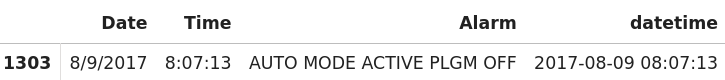
\includegraphics[width=0.7\linewidth]{files/CSE572_Fig_1-399d284a5dea92b7f0447a4ec4a2d281.png}
\caption[]{Insulin Pump Auto Mode Data Row}
\label{CSE572_Fig_1}
\end{figure}

The corresponding data point with the closest time stamp in the CGM sensor dataset is shown in Figure~\ref{CSE572_Fig_2}: Corresponding CGM Sensor Auto Mode Data Row:

\begin{figure}[!htbp]
\centering
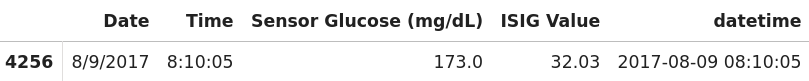
\includegraphics[width=0.7\linewidth]{files/CSE572_Fig_2-44bb7ee06feb7f47ad9bc48a3b265920.png}
\caption[]{Corresponding CGM Sensor Auto Mode Data Row}
\label{CSE572_Fig_2}
\end{figure}

In order to visualize the CGM sensor data, a plot was made using Pandas.  On the x -- axis we have the row number, and on the y -- axis we have the sensor glucose output in [mg/dL] as shown in Figure~\ref{CSE572_Fig_3}: Plot of CGM Data vs Row Number.

\begin{figure}[!htbp]
\centering
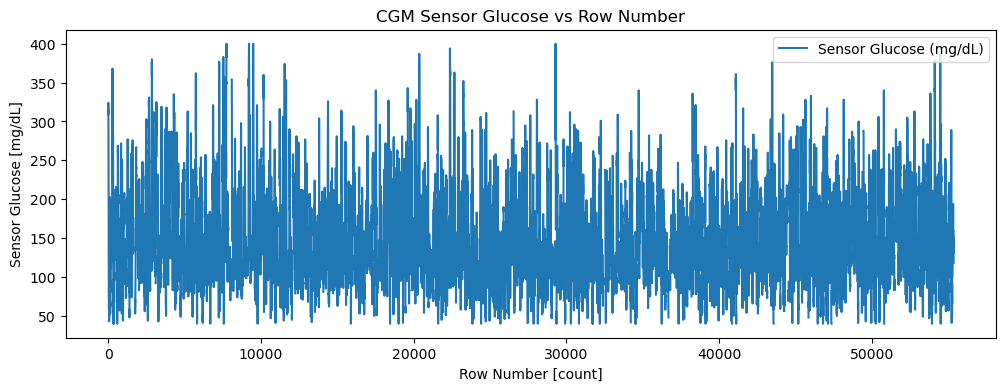
\includegraphics[width=0.7\linewidth]{files/CSE572_Fig_3-172aea5bcbe5fa91bdbd521680f2d239.png}
\caption[]{Plot of CGM Data vs Row Number}
\label{CSE572_Fig_3}
\end{figure}

Not much can be seen from the plot in Figure~\ref{CSE572_Fig_3}: Plot of CGM Data vs Row Number at this point, except for maybe the minimums and maximums.

The CGM data was processed and placed into a \texttt{Pandas}\footnote{Pandas. \href{https://pandas.pydata.org/}{https://pandas.pydata.org/}} \texttt{Dataframe}\footnote{A \texttt{DataFrame} is a two-dimensional, size-mutable, and potentially heterogeneous tabular data structure provided by the Pandas Python module, which allows for easy data manipulation, analysis, and storage in rows and columns. \href{https://pandas.pydata.org/pandas-docs/stable/reference/api/pandas.DataFrame.html}{https://pandas.pydata.org/pandas-docs/stable/reference/api/pandas.DataFrame.html}} shown in Figure~\ref{CSE572_Fig_4}: Processed CGM Dataframe:

\begin{figure}[!htbp]
\centering
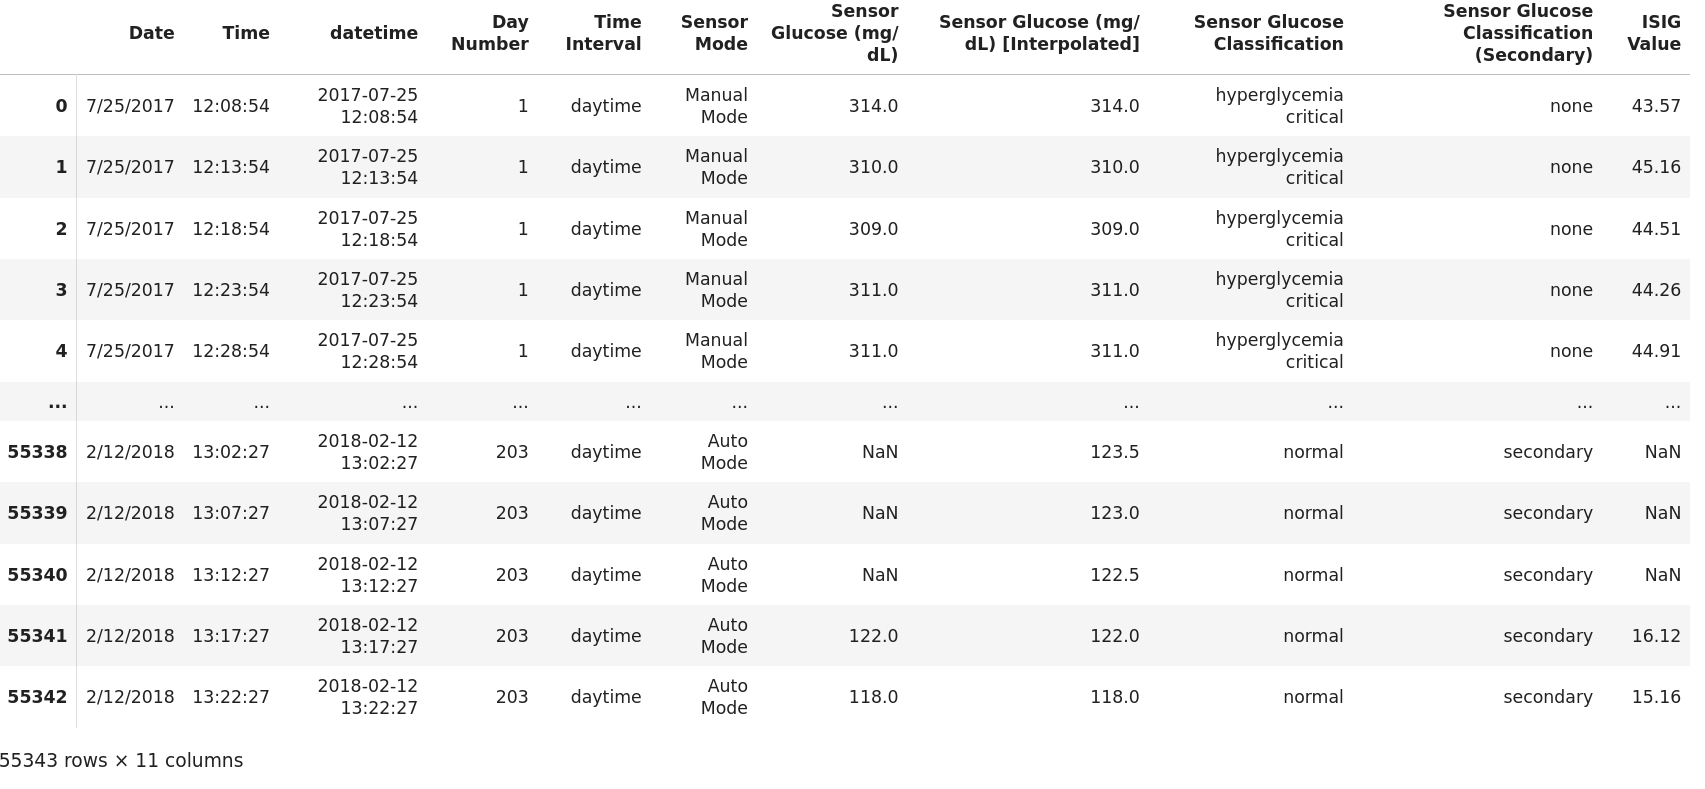
\includegraphics[width=0.7\linewidth]{files/CSE572_Fig_4-ef36140a4a772a57166d78ada15d780b.png}
\caption[]{Processed CGM Dataframe}
\label{CSE572_Fig_4}
\end{figure}

To obtain the averages required for the Project, sub -- dataframes were selected from the main dataframe shown in Figure~\ref{CSE572_Fig_4}: Processed CGM Dataframe based on the required mean.  For example, Manual Mode, Overnight Percentage of Time in Hyperglycemia range.  There were 166 CGM entries spanning 7 distinct days.  This data was aggregated by day using the \texttt{Pandas}\footnote{Pandas. \href{https://pandas.pydata.org/}{https://pandas.pydata.org/}} \texttt{groupby}\footnote{The \texttt{groupby()} function in the Pandas Python module is used to split data into groups based on some criteria, allowing for aggregation, transformation, or filtration of the data within each group. \href{https://pandas.pydata.org/pandas-docs/stable/reference/api/pandas.DataFrame.groupby.html}{https://pandas.pydata.org/pandas-docs/stable/reference/api/pandas.DataFrame.groupby.html}} function and counted to obtain the quantity in hyperglycemia for that day.  This is shown in Figure~\ref{CSE572_Fig_5}: Manual Mode / Overnight / Hyperglycemia.

\begin{figure}[!htbp]
\centering
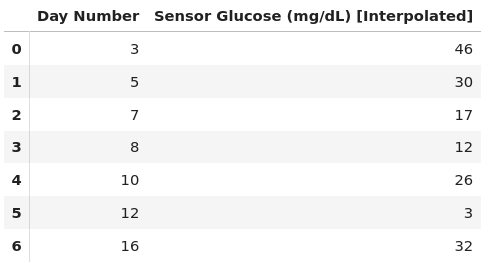
\includegraphics[width=0.7\linewidth]{files/CSE572_Fig_5-c29003ca3dd7d0b574c577ef0d9298e0.png}
\caption[]{Manual Mode / Overnight / Hyperglycemia}
\label{CSE572_Fig_5}
\end{figure}

The percentage mean for the day was computed by dividing each row in Figure~\ref{CSE572_Fig_5}: Manual Mode / Overnight / Hyperglycemia by 288 and multiplying by 100.  An overall mean for this set of conditions was obtained by averaging the percentage mean for each day out of the total number of days in the the dataset.  Similar methodoly was undertaken for the 35 other combinations.  The results of all of the means for the 36 combinations are given in Project~1~Results~-~Table~of~Calculated~Percentage~Means:~Overnight, Project~1~Results~-~Table~of~Calculated~Percentage~Means:~Daytime and Project~1~Results~-~Table~of~Calculated~Percentage~Means:~Whole~Day:

\begin{verbatim}
output_df[column_names_overnight]
\end{verbatim}

\bigskip\noindent
\begin{tabular}{p{\dimexpr 0.143\linewidth-2\tabcolsep}p{\dimexpr 0.143\linewidth-2\tabcolsep}p{\dimexpr 0.143\linewidth-2\tabcolsep}p{\dimexpr 0.143\linewidth-2\tabcolsep}p{\dimexpr 0.143\linewidth-2\tabcolsep}p{\dimexpr 0.143\linewidth-2\tabcolsep}p{\dimexpr 0.143\linewidth-2\tabcolsep}}
\toprule
 & Overnight Hyperglycemia [\% of time] & Overnight Hyperglycemia Critical [\% of time] & Overnight Normal [\% of time] & Overnight Secondary [\% of time] & Overnight Hypoglycemia Level 1 [\% of time] & Overnight Hypoglycemia Level 2 [\% of time] \\
\hline
Manual Mode & 0.283935 & 0.076970 & 1.436782 & 1.069034 & 0.049603 & 0.000000 \\
\hline
Auto Mode & 2.175698 & 0.405378 & 18.756842 & 16.379310 & 0.401957 & 0.191571 \\
\hline
\bottomrule
\end{tabular}

\bigskip

\begin{verbatim}
output_df[column_names_daytime]
\end{verbatim}

\bigskip\noindent
\begin{tabular}{p{\dimexpr 0.143\linewidth-2\tabcolsep}p{\dimexpr 0.143\linewidth-2\tabcolsep}p{\dimexpr 0.143\linewidth-2\tabcolsep}p{\dimexpr 0.143\linewidth-2\tabcolsep}p{\dimexpr 0.143\linewidth-2\tabcolsep}p{\dimexpr 0.143\linewidth-2\tabcolsep}p{\dimexpr 0.143\linewidth-2\tabcolsep}}
\toprule
 & Daytime Hyperglycemia [\% of time] & Daytime Hyperglycemia Critical [\% of time] & Daytime Normal [\% of time] & Daytime Secondary [\% of time] & Daytime Hypoglycemia Level 1 [\% of time] & Daytime Hypoglycemia Level 2 [\% of time] \\
\hline
Manual Mode & 1.311918 & 0.725233 & 3.018952 & 2.360427 & 0.225780 & 0.150520 \\
\hline
Auto Mode & 14.516626 & 4.354817 & 43.402778 & 32.337849 & 2.138068 & 1.038246 \\
\hline
\bottomrule
\end{tabular}

\bigskip

\begin{verbatim}
output_df[column_names_whole_day]
\end{verbatim}

\bigskip\noindent
\begin{tabular}{p{\dimexpr 0.143\linewidth-2\tabcolsep}p{\dimexpr 0.143\linewidth-2\tabcolsep}p{\dimexpr 0.143\linewidth-2\tabcolsep}p{\dimexpr 0.143\linewidth-2\tabcolsep}p{\dimexpr 0.143\linewidth-2\tabcolsep}p{\dimexpr 0.143\linewidth-2\tabcolsep}p{\dimexpr 0.143\linewidth-2\tabcolsep}}
\toprule
 & Whole Day Hyperglycemia [\% of time] & Whole Day Hyperglycemia Critical [\% of time] & Whole Day Normal [\% of time] & Whole Day Secondary [\% of time] & Whole Day Hypoglycemia Level 1 [\% of time] & Whole Day Hypoglycemia Level 2 [\% of time] \\
\hline
Manual Mode & 1.595854 & 0.802203 & 4.455733 & 3.429461 & 0.275383 & 0.150520 \\
\hline
Auto Mode & 16.692323 & 4.760194 & 62.159620 & 48.717159 & 2.540025 & 1.229817 \\
\hline
\bottomrule
\end{tabular}

\bigskip

It can be seen from Project~1~Results~-~Table~of~Calculated~Percentage~Means:~Overnight, Project~1~Results~-~Table~of~Calculated~Percentage~Means:~Daytime and Project~1~Results~-~Table~of~Calculated~Percentage~Means:~Whole~Day that the person spent a majority of their time in either the normal or secondary ranges while in Auto Mode.  The numbers were non -- sensical for Manual Mode, perhaps because the person was not recording data.

\subparagraph{Project 2: Machine Model Training Project}

The Meal and No Meal Data Matrices were extracted from the CGM sensor datasets.  A heatmap of the cleaned, imputed meal data matrix is shown in Figure~\ref{CSE572_Fig_6}: Heatmap of Meal Data Matrix 1:

\begin{figure}[!htbp]
\centering
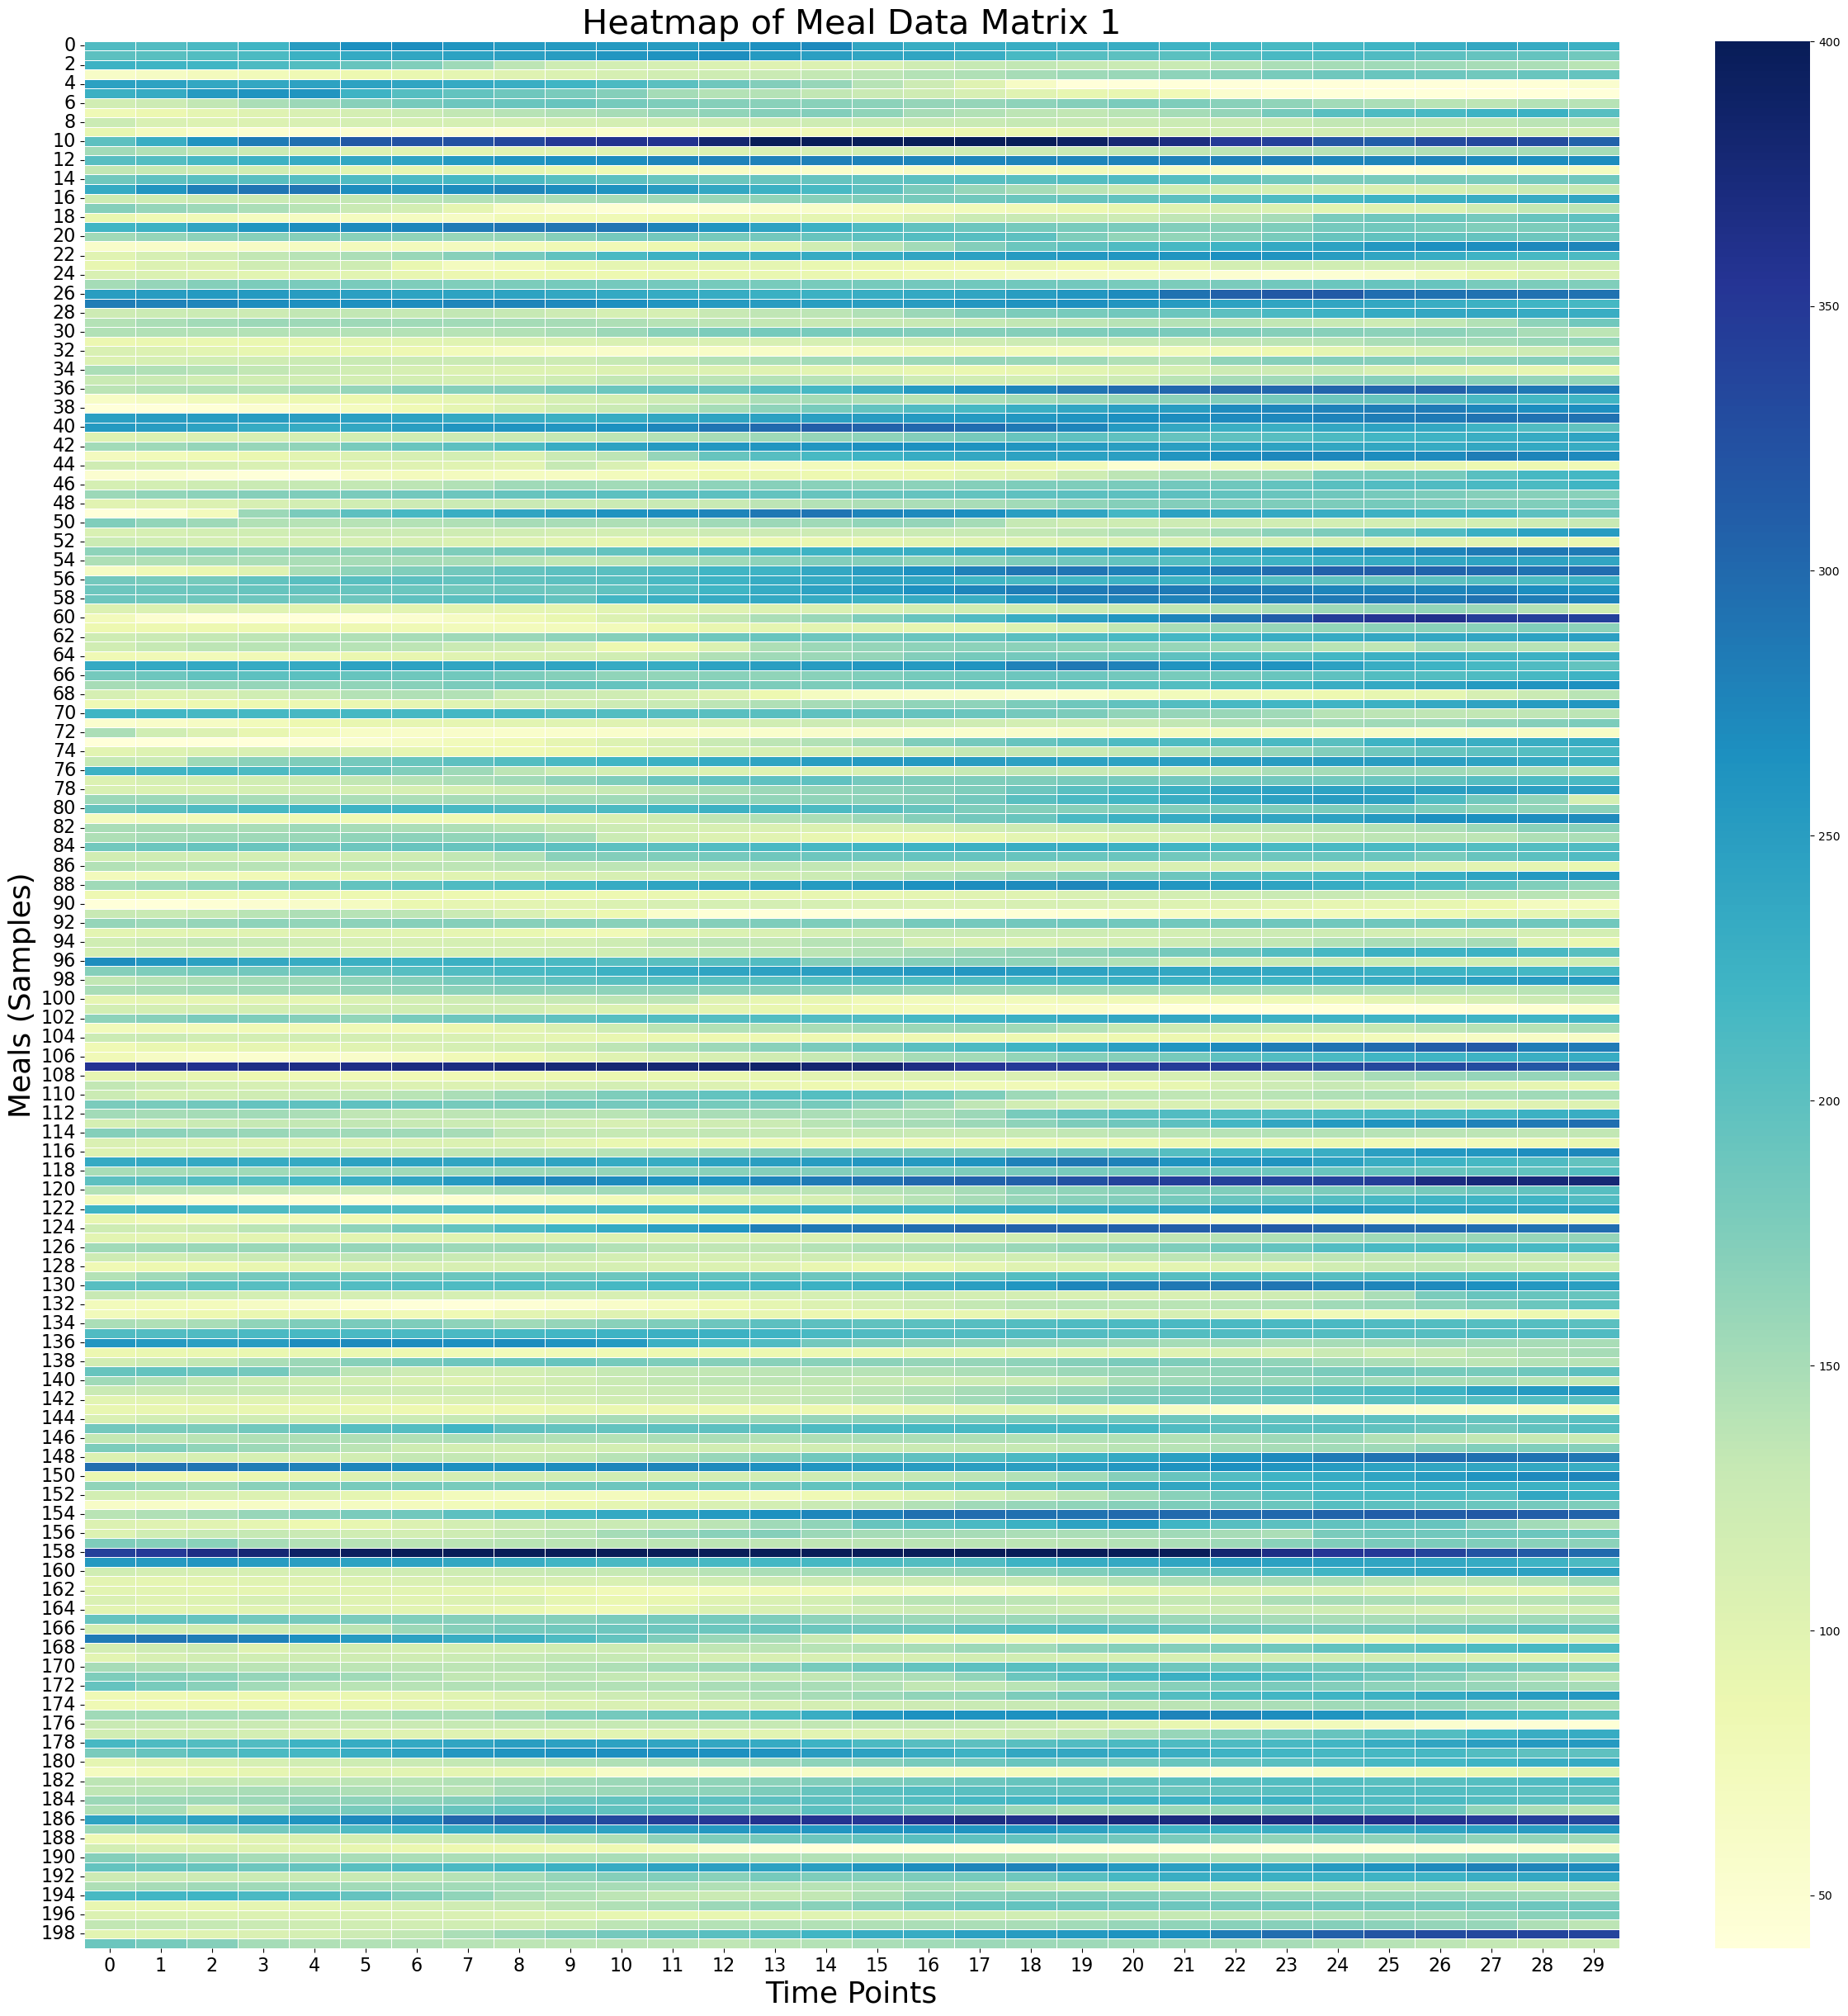
\includegraphics[width=0.7\linewidth]{files/CSE572_Fig_6-f6f24221ecee5c5fbd655b4ddecc543a.png}
\caption[]{Heatmap of Meal Data Matrix 1}
\label{CSE572_Fig_6}
\end{figure}

Features were extracted from the Meal Data Matrix using a feature~extractor function:

\begin{verbatim}
def feature_extractor(data_matrix):

    features = []

    for row in data_matrix:
        mean_glucose = np.mean(row)
        std_glucose  = np.std(row)
        max_glucose  = np.max(row)
        min_glucose  = np.min(row)
        
        first_derivative = compute_first_derivative(row)
        mean_first_derivate = np.mean(first_derivative)

        if len(row) > 2:
            second_derivative = compute_second_derivative(row)
            mean_second_derivative = np.mean(second_derivative)
        else:
            mean_second_derivative = 0

        AUC = compute_AUC(row)

        time_to_peak = np.argmax(row)

        features_vector = [
            mean_glucose,
            std_glucose,
            max_glucose,
            min_glucose,
            mean_first_derivate,
            mean_second_derivative,
            AUC,
            time_to_peak
        ]

        features.append(features_vector)
    
    return np.array(features)
\end{verbatim}

A moving average visulization of the row Maximum, Average, Minimum and Standard Deviation are shown in Figure~\ref{CSE572_Fig_7}: Moving Average of  the Maximum, Mean, Standard Deviation and Minimum of the Meal Features Matrix Rows.

\begin{figure}[!htbp]
\centering
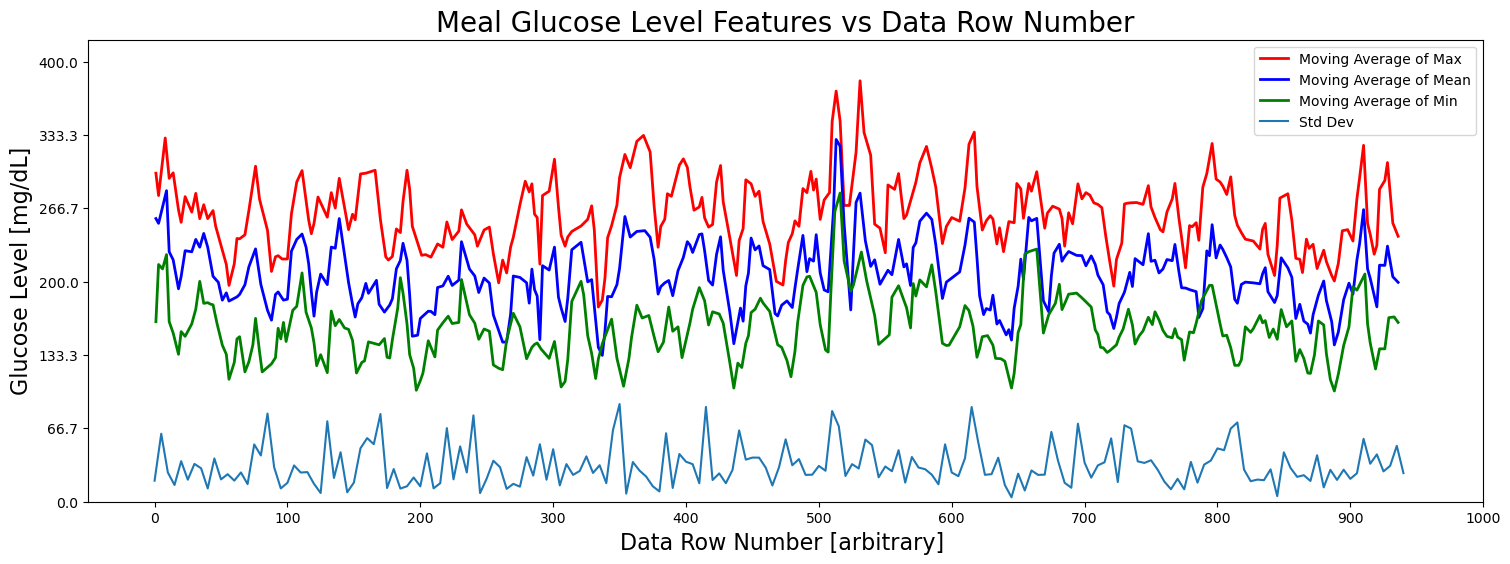
\includegraphics[width=0.7\linewidth]{files/CSE572_Fig_7-2f70bee886a530c03e30d9907acf9120.png}
\caption[]{Moving Average of  the Maximum, Mean, Standard Deviation and Minimum of the Meal Features Matrix Rows}
\label{CSE572_Fig_7}
\end{figure}

The \texttt{Seaborn}\footnote{\texttt{Seaborn} is a Python data visualization library based on Matplotlib that provides a high-level interface for creating attractive and informative statistical graphics. \href{https://seaborn.pydata.org/}{https://seaborn.pydata.org/}} \texttt{Pandas}\footnote{Pandas. \href{https://pandas.pydata.org/}{https://pandas.pydata.org/}} module was used to produce a \texttt{pairwise plot}\footnote{\texttt{Pairwise Plotting} is a data visualization technique that involves creating scatter plots for every possible pair of variables in a dataset, allowing for the examination of relationships and correlations between multiple variables simultaneously. \href{https://seaborn.pydata.org/generated/seaborn.pairplot.html}{https://seaborn.pydata.org/generated/seaborn.pairplot.html}} of the eight extrated features.  This plot is shown in Figure~\ref{CSE572_Fig_8}: Pairwise Plot of Meal Features Matrix.

\begin{figure}[!htbp]
\centering
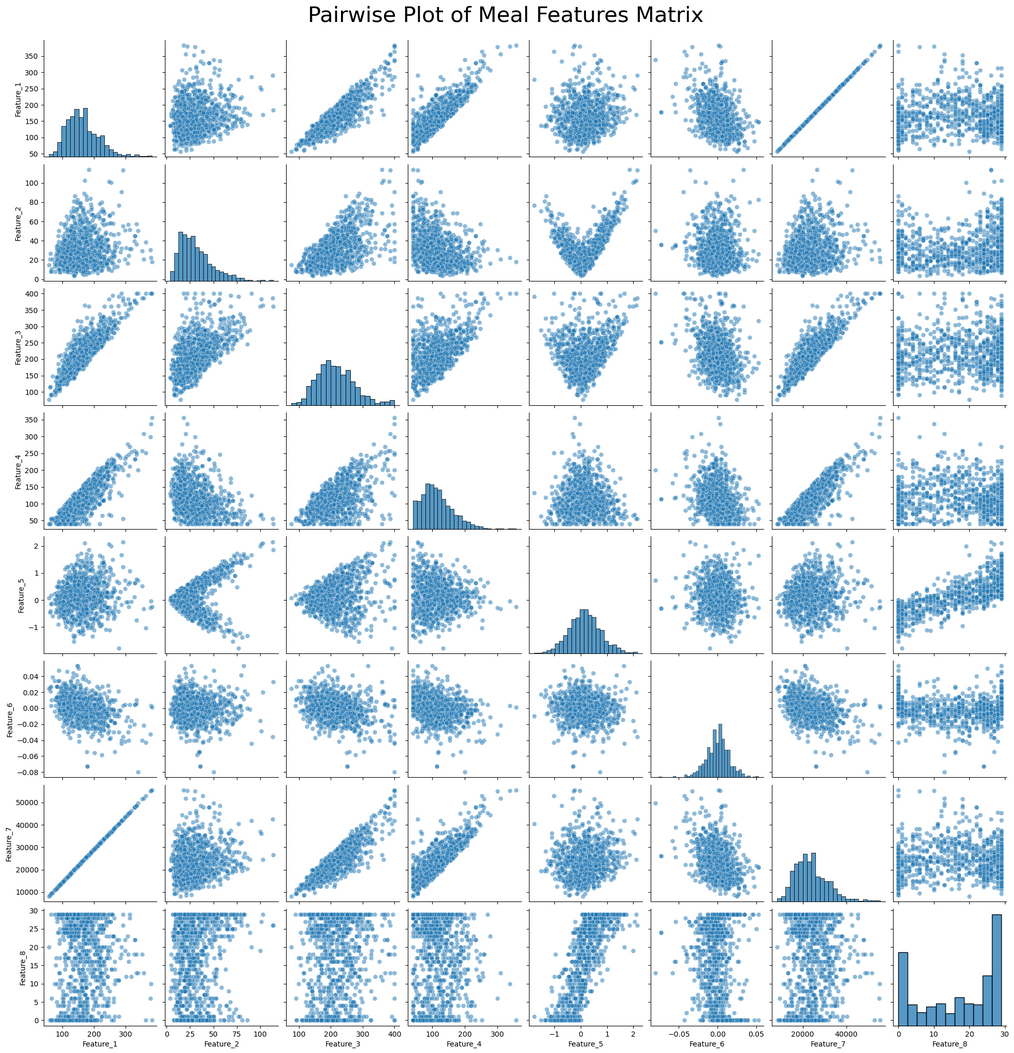
\includegraphics[width=0.7\linewidth]{files/CSE572_Fig_8-6e400a5896a5d383ce0182814998f4e4.png}
\caption[]{Pairwise Plot of Meal Features Matrix}
\label{CSE572_Fig_8}
\end{figure}

It can be seen in Figure~\ref{CSE572_Fig_8}: Pairwise Plot of Meal Features Matrix that there is a strong positive linear correlation between Feature 1 (row mean) and Feature 7 (area under curve).

For the No Meal Features Matrix, features were extracted from the using the same feature extractor function.  A moving average visulization of the row Maximum, Average, Minimum and Standard Deviation are shown in Figure~\ref{CSE572_Fig_9}: Moving Average of  the Maximum, Mean, Standard Deviation and Minimum of the No Meal Features Matrix Rows.

\begin{figure}[!htbp]
\centering
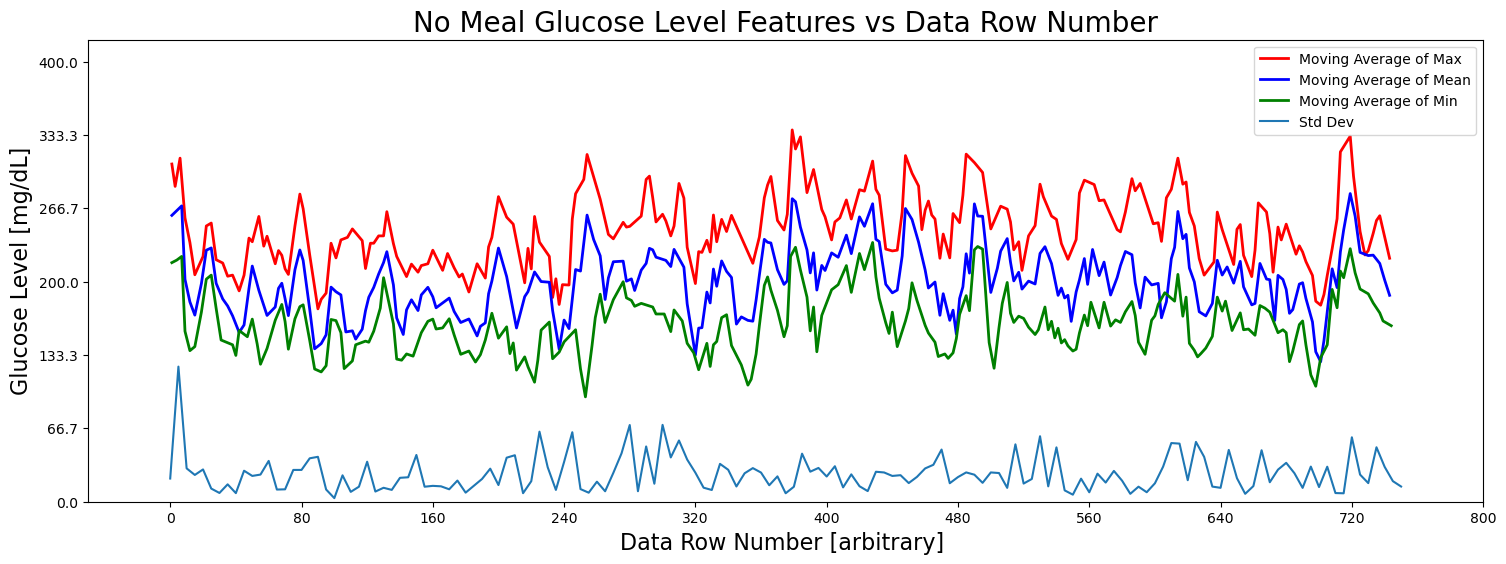
\includegraphics[width=0.7\linewidth]{files/CSE572_Fig_9-71442b7dd22546e55d13acbc051d50b9.png}
\caption[]{Moving Average of  the Maximum, Mean, Standard Deviation and Minimum of the No Meal Features Matrix Rows}
\label{CSE572_Fig_9}
\end{figure}

At first glance it appears that it would be difficult to visually discern whether a meal has occurred when comparing Figure~\ref{CSE572_Fig_7}: Moving Average of the Maximum, Mean, Standard Deviation and Minimum of the Meal Features Matrix Rows and Figure~\ref{CSE572_Fig_9}: Moving Average of  the Maximum, Mean, Standard Deviation and Minimum of the No Meal Features Matrix Rows.  As for the Meal Features Matrix, a \texttt{pairwise plot}\footnote{\texttt{Pairwise Plotting} is a data visualization technique that involves creating scatter plots for every possible pair of variables in a dataset, allowing for the examination of relationships and correlations between multiple variables simultaneously. \href{https://seaborn.pydata.org/generated/seaborn.pairplot.html}{https://seaborn.pydata.org/generated/seaborn.pairplot.html}} was created for the No Meal Features Matrix, shown in Figure~\ref{CSE572_Fig_10}: Pairwise Plot of No Meal Features Matrix.

\begin{figure}[!htbp]
\centering
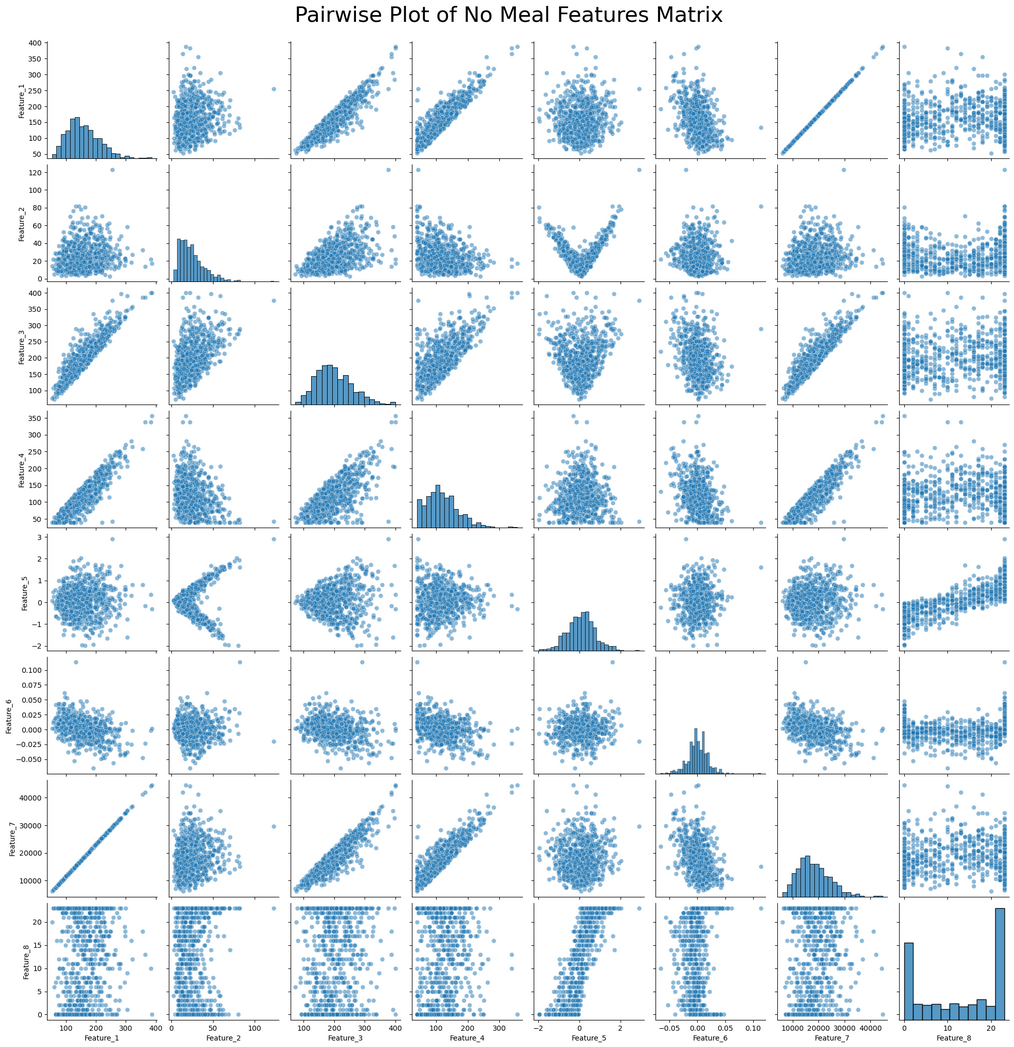
\includegraphics[width=0.7\linewidth]{files/CSE572_Fig_10-563e9e4cc992eab2a203317c2c0fe5bf.png}
\caption[]{Pairwise Plot of No Meal Features Matrix}
\label{CSE572_Fig_10}
\end{figure}

In Figure~\ref{CSE572_Fig_10}: Pairwise Plot of No Meal Features Matrix, we again observe a strong positive linear  correlation between Feature 1 (row mean) and Feature 7 (area under curve).

The meal and no meal feature matrices were vertically stacked, normalized and class lables were appended. A Sklearn\footnote{Scikit-learn. \href{https://scikit-learn.org/}{https://scikit-learn.org/}} \texttt{Support Vector Machine (SVM)}\footnote{A \texttt{Support Vector Machine (SVM)} is a supervised machine learning model that uses classification algorithms for two-group classification problems. After giving an SVM model sets of labeled training data for each category, they're able to categorize new text. \href{https://en.wikipedia.org/wiki/Support\_vector\_machine}{Support vector machine}} machine learning model was then trained on the features data using a train / test split ratio of 80\% / 20\%, respectively.

The \texttt{SVM}\footnote{A \texttt{Support Vector Machine (SVM)} is a supervised machine learning model that uses classification algorithms for two-group classification problems. After giving an SVM model sets of labeled training data for each category, they're able to categorize new text. \href{https://en.wikipedia.org/wiki/Support\_vector\_machine}{Support vector machine}} model was then tested on the test data and surprisingly had a test accuracy of 99.71\%, with an \href{https://grokipedia.com/page/F-score}{F1 score} of 1.00.  A visual representation of the model's prediction accuracy was generated by using \texttt{Principle Component Analysis (PCA)}\footnote{\texttt{Principal Component Analysis (PCA)} is a statistical procedure that uses an orthogonal transformation to convert a set of observations of possibly correlated variables into a set of values of linearly uncorrelated variables called principal components. \href{https://en.wikipedia.org/wiki/Principal\_component\_analysis}{Principal component analysis}} on the scaled test data.  The results are shown in Figure~\ref{CSE572_Fig_11}: SVM Classification Results: Correct vs Incorrect Predictions on Test Data.

\begin{figure}[!htbp]
\centering
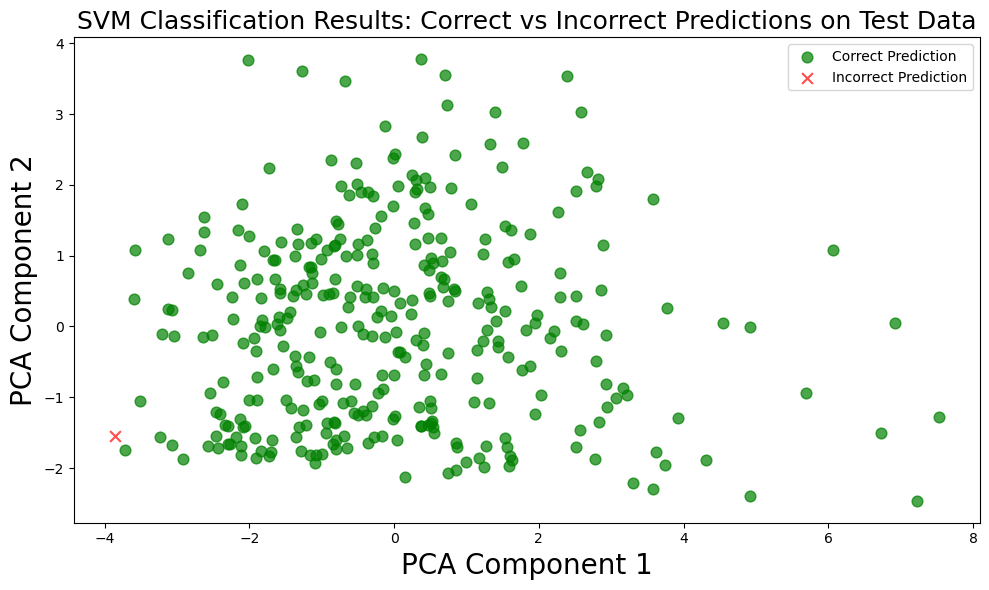
\includegraphics[width=0.7\linewidth]{files/CSE572_Fig_11-df72b07d5e4b8bccce782158459ba65f.png}
\caption[]{SVM Classification Results: Correct vs Incorrect Predictions on Test Data}
\label{CSE572_Fig_11}
\end{figure}

The reason for this remarkable result is thought to be the selection of features that enabled the SVM machine to definitively differentiate between a meal and a no meal data sample.  To test this theory, a Seaborn pair plot was generated on the features data and the predicted class.  This plot is shown in Figure~\ref{CSE572_Fig_12}: Pair Plot of SVM Classification Results.

\begin{figure}[!htbp]
\centering
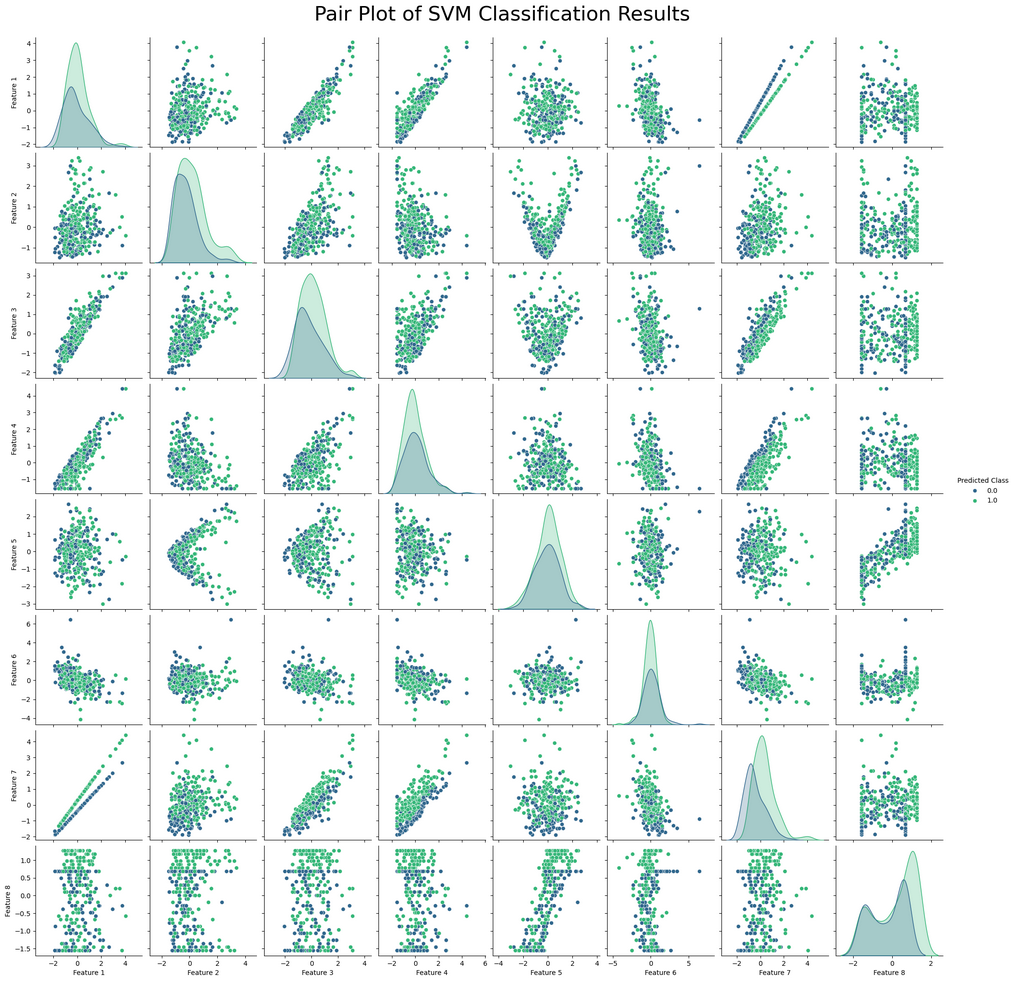
\includegraphics[width=0.7\linewidth]{files/CSE572_Fig_12-2afa079f836e264fdf0a9afeab0bdd0a.png}
\caption[]{Pair Plot of SVM Classification Results}
\label{CSE572_Fig_12}
\end{figure}

The pair plot in Figure~\ref{CSE572_Fig_12}: Pair Plot of \texttt{SVM}\footnote{A \texttt{Support Vector Machine (SVM)} is a supervised machine learning model that uses classification algorithms for two-group classification problems. After giving an SVM model sets of labeled training data for each category, they're able to categorize new text. \href{https://en.wikipedia.org/wiki/Support\_vector\_machine}{Support vector machine}} Classification Results again shows a strong positive linear correlation between Feature 1 (row mean) and Feature 7 (area under curve).  The plot also shows that for Feature 7 (area under curve), there is substantial non -- overlap of the histogram distributions.  This allows the \texttt{SVM} machine to accurately predict whether the features data object is a meal or a non -- meal data object.

Lastly, a \texttt{Confusion Matrix Heatmap}\footnote{\texttt{Principal Component Analysis (PCA)} is a statistical procedure that uses an orthogonal transformation to convert a set of observations of possibly correlated variables into a set of values of linearly uncorrelated variables called principal components. \href{https://en.wikipedia.org/wiki/Principal\_component\_analysis}{Principal component analysis}} was created to visualize the \texttt{SVM} machine's \href{https://grokipedia.com/page/Machine\_learning\#evaluation-and-validation}{\texttt{accuracy}}, \href{https://grokipedia.com/page/Precision\_and\_recall}{\texttt{recall}}, \href{https://grokipedia.com/page/Precision\_and\_recall}{\texttt{precision}} and \href{https://grokipedia.com/page/Machine\_learning\#evaluation-and-validation}{\texttt{F1 score}}.  These results are shown in Figure~\ref{CSE572_Fig_13}: Confusion Matrix Heatmap of Test Data:

\begin{figure}[!htbp]
\centering
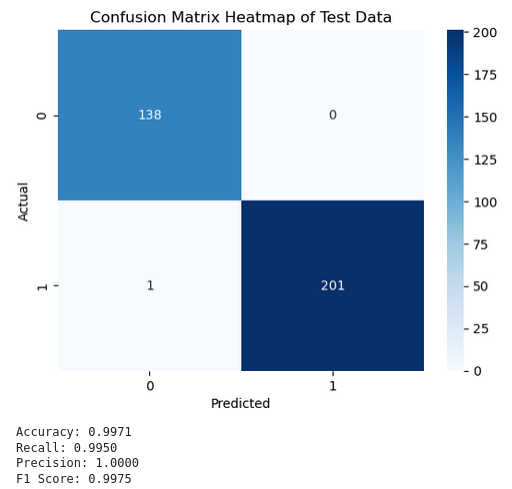
\includegraphics[width=0.7\linewidth]{files/CSE572_Fig_13-50184137761a5951b5d6f367525f48bd.png}
\caption[]{Confusion Matrix Heatmap of Test Data}
\label{CSE572_Fig_13}
\end{figure}

\subparagraph{Project 3: Cluster Validation Project}

A method similar to Project 2 was used to extract the meal carbohydrate ingestion data from the Insulin Pump dataset.  The extracted carbohydrate amounts were then binned into six bins that were bounded by the minimum and maximum carbohydrate ingestion amounts.  This resulted in the ``ground truth'' that will be later employed for cluster validation.

Addtionally, using methods similar to Project 2, the meal blood glucose levels were extracted from the CGM sensor dataset.  The data was then cleaned and missing data items were \href{https://grokipedia.com/page/Imputation\_(statistics)}{imputed} using Sklearn's\footnote{Scikit-learn. \href{https://scikit-learn.org/}{https://scikit-learn.org/}} \texttt{KNN Imputer}\footnote{The \texttt{KNNImputer} class in the Sklearn Python module provides imputation for completing missing values using the k-Nearest Neighbors approach. \href{https://scikit-learn.org/stable/modules/generated/sklearn.impute.KNNImputer.html}{https://scikit-learn.org/stable/modules/generated/sklearn.impute.KNNImputer.html}}.  Features were then extracted from the meal blood glucose sensor readins in a manner similar to what was employed in Project 2.  The features were then normalized to facilitate accurate clustering.

\texttt{K-Means Clustering}\footnote{\texttt{K-Means} is an unsupervised machine learning algorithm used for clustering data into K distinct groups based on feature similarity. \href{https://en.wikipedia.org/wiki/K-means\_clustering}{K-means clustering}} was employed first.  The clustering results were plotted against two \href{https://grokipedia.com/page/Principal\_component\_analysis}{Principle Components} features that were obtained using \href{https://grokipedia.com/page/Principal\_component\_analysis}{\texttt{Principle Component Analysis (PCA)}}\footnote{\texttt{Principal Component Analysis (PCA)} is a statistical procedure that uses an orthogonal transformation to convert a set of observations of possibly correlated variables into a set of values of linearly uncorrelated variables called principal components. \href{https://en.wikipedia.org/wiki/Principal\_component\_analysis}{Principal component analysis}} from \texttt{Sklearn's}\footnote{Scikit-learn. \href{https://scikit-learn.org/}{https://scikit-learn.org/}} \texttt{PCA}\footnote{The \texttt{PCA} class in the Sklearn Python module is used to perform Principal Component Analysis, a dimensionality reduction technique that transforms data into a new coordinate system by identifying the directions (principal components) that maximize variance. \href{https://scikit-learn.org/stable/modules/generated/sklearn.decomposition.PCA.html}{https://scikit-learn.org/stable/modules/generated/sklearn.decomposition.PCA.html}} class.  The plotted results are shown in Figure~\ref{CSE572_Fig_14}: K - Means Clusters vs PCA Components:

\begin{figure}[!htbp]
\centering
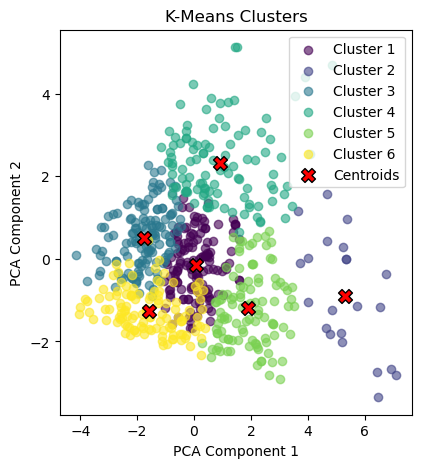
\includegraphics[width=0.7\linewidth]{files/CSE572_Fig_14-b51ef0a34aab48036b0de91972196857.png}
\caption[]{K - Means Clusters vs PCA Components}
\label{CSE572_Fig_14}
\end{figure}

In order to assess the validity of the clustering, a dual plot was generated of the original bins and the results of the K -- Means clustering.  The result is shown in Figure~\ref{CSE572_Fig_15}: Original Bins and K - Means Clustering Bins:

\begin{figure}[!htbp]
\centering
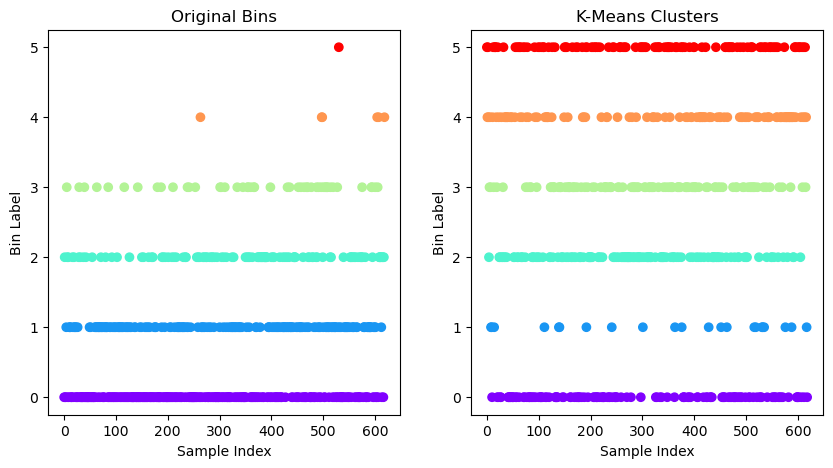
\includegraphics[width=0.7\linewidth]{files/CSE572_Fig_15-4369192b8511254bbb4fb7ca710d9be5.png}
\caption[]{Original Bins and K - Means Clustering Bins}
\label{CSE572_Fig_15}
\end{figure}

It can be seen from Figure~\ref{CSE572_Fig_15}: Original Bins and K - Means Clustering Bins heavily mis -- clustered bins 1 and 4.  The \texttt{Sum of the Squared Error (SSE)}\footnote{The \texttt{Sum of Squared Errors (SSE)} is a statistical measure used to quantify the total deviation of predicted values from the actual values in a dataset, calculated by summing the squares of the differences between each predicted value and its corresponding actual value. \href{https://en.wikipedia.org/wiki/Residual\_sum\_of\_squares}{Residual sum of squares}} for the \texttt{K -- Means Clustering}\footnote{\texttt{K-Means} is an unsupervised machine learning algorithm used for clustering data into K distinct groups based on feature similarity. \href{https://en.wikipedia.org/wiki/K-means\_clustering}{K-means clustering}} result is shown in  K~-~Means~SSE~Result.

\begin{verbatim}
# Compute SSE
SSE_kmeans = np.float64(kmeans.inertia_)
SSE_kmeans
\end{verbatim}

\begin{verbatim}
np.float64(1840.9904638055532)
\end{verbatim}

DBSCAN clustering was then performed.  A plot of the \texttt{DBSCAN}\footnote{\texttt{DBSCAN} (Density-Based Spatial Clustering of Applications with Noise) is an unsupervised machine learning algorithm used for clustering data points based on their density, allowing it to identify clusters of varying shapes and sizes while effectively handling noise and outliers. \href{https://en.wikipedia.org/wiki/DBSCAN}{DBSCAN}} clustering results were plotted against two \href{https://grokipedia.com/page/Principal\_component\_analysis}{Principle Components} of the features matrix and shown side -- by -- side with the \texttt{K -- Means Clustering}\footnote{\texttt{K-Means} is an unsupervised machine learning algorithm used for clustering data into K distinct groups based on feature similarity. \href{https://en.wikipedia.org/wiki/K-means\_clustering}{K-means clustering}} results for comparison.  This is shown in Figure~\ref{CSE572_Fig_16}: DBSCAN Clustering and K - Means Clustering Results:

\begin{figure}[!htbp]
\centering
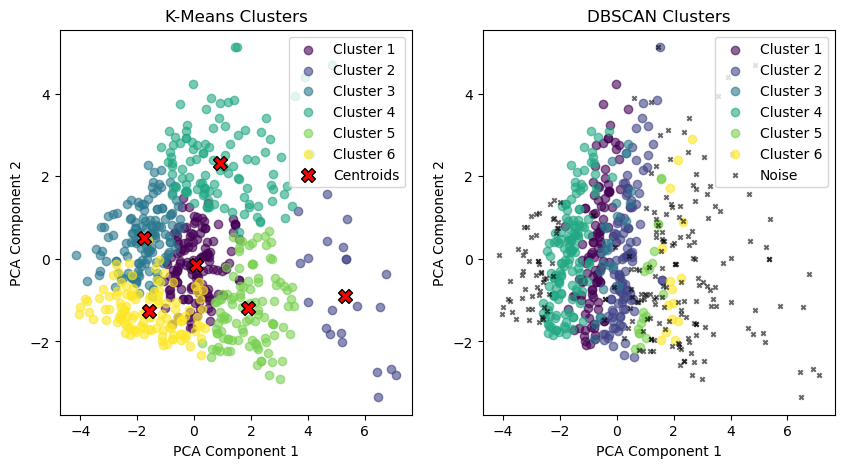
\includegraphics[width=0.7\linewidth]{files/CSE572_Fig_16-cd6b8f78b6363de68402b26390554727.png}
\caption[]{DBSCAN Clustering and K - Means Clustering Results}
\label{CSE572_Fig_16}
\end{figure}

Notably, the \texttt{DBSCAN}\footnote{\texttt{DBSCAN} (Density-Based Spatial Clustering of Applications with Noise) is an unsupervised machine learning algorithm used for clustering data points based on their density, allowing it to identify clusters of varying shapes and sizes while effectively handling noise and outliers. \href{https://en.wikipedia.org/wiki/DBSCAN}{DBSCAN}} clustering results shown in Figure~\ref{CSE572_Fig_16} are very different than the \texttt{K -- Means Clustering}\footnote{\texttt{K-Means} is an unsupervised machine learning algorithm used for clustering data into K distinct groups based on feature similarity. \href{https://en.wikipedia.org/wiki/K-means\_clustering}{K-means clustering}} results.  This can be explained because \texttt{DBSCAN} works off of data density rather than distance to the initially guessed \href{https://grokipedia.com/page/K-means\_clustering\#k--means-clustering}{\texttt{centroid}} as in \texttt{K -- Means Clustering}.  To assess whether the \texttt{DBSCAN} clustering was able to properly cluster the features data, a dual plot was generated of the original bins and the results of the \texttt{DBSCAN} clustering.  The result is shown in Figure~\ref{CSE572_Fig_17}: Original Bins and DBSCAN Clustering Bins:

\begin{figure}[!htbp]
\centering
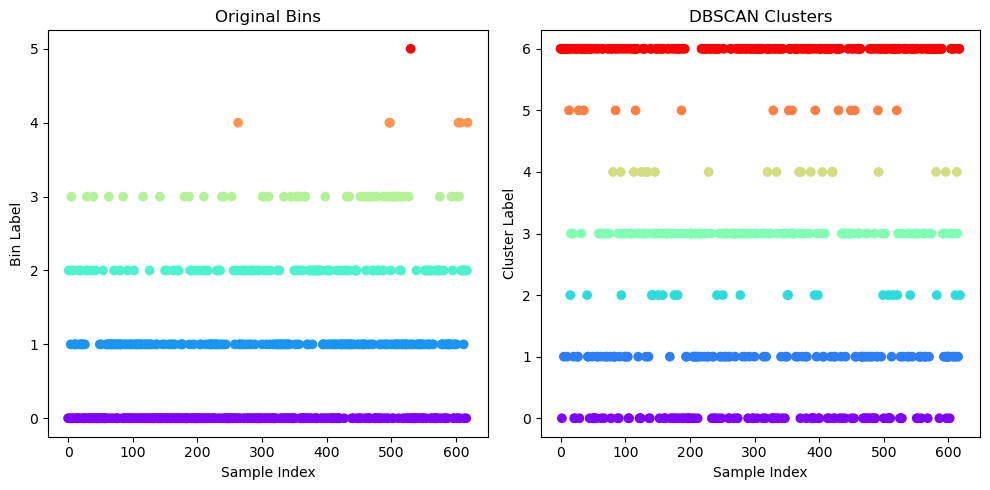
\includegraphics[width=0.7\linewidth]{files/CSE572_Fig_17-a8036b67a586d300d54445067f2aa045.png}
\caption[]{Original Bins and DBSCAN Clustering Bins}
\label{CSE572_Fig_17}
\end{figure}

It can be seen from Figure~\ref{CSE572_Fig_17}: Original Bins and DBSCAN Clustering Bins heavily mis -- clustered bins 1 and 4.  The \texttt{Sum of the Squared Error (SSE)}\footnote{The \texttt{Sum of Squared Errors (SSE)} is a statistical measure used to quantify the total deviation of predicted values from the actual values in a dataset, calculated by summing the squares of the differences between each predicted value and its corresponding actual value. \href{https://en.wikipedia.org/wiki/Residual\_sum\_of\_squares}{Residual sum of squares}} for the \texttt{DBSCAN}\footnote{\texttt{DBSCAN} (Density-Based Spatial Clustering of Applications with Noise) is an unsupervised machine learning algorithm used for clustering data points based on their density, allowing it to identify clusters of varying shapes and sizes while effectively handling noise and outliers. \href{https://en.wikipedia.org/wiki/DBSCAN}{DBSCAN}} clustering result is shown in DBSCAN~Clustering~SSE.

\begin{verbatim}
# Get unique clusters excluding noise ( -1)
unique_clusters = set(y_dbscan) - { -1}

# Initialize SSE
SSE_dbscan = 0

# Loop over each cluster to compute SSE
for cluster in unique_clusters:
    # Get points in the current cluster
    cluster_points = meal_glucose_features_matrix[y_dbscan == cluster]
    
    # Compute the pseudo -centroid (mean of points in the cluster)
    pseudo_centroid = np.mean(cluster_points, axis=0)
    
    # Compute SSE for this cluster
    sse_cluster = np.sum((cluster_points - pseudo_centroid) ** 2)
    
    # Add the cluster's SSE to the total SSE
    SSE_dbscan += sse_cluster

print(f"Approximate SSE for DBSCAN (excluding noise): {SSE_dbscan}")
\end{verbatim}

\begin{verbatim}
Approximate SSE for DBSCAN (excluding noise): 365871520.5756363
\end{verbatim}

The cluster and overall \href{https://towardsdatascience.com/evaluation-metrics-for-clustering-models-5dde821dd6cd/}{\texttt{Total Entropy and Purity}} were computed for both the \texttt{K -- Means Clustering}\footnote{\texttt{K-Means} is an unsupervised machine learning algorithm used for clustering data into K distinct groups based on feature similarity. \href{https://en.wikipedia.org/wiki/K-means\_clustering}{K-means clustering}} and \texttt{DBSCAN}\footnote{\texttt{DBSCAN} (Density-Based Spatial Clustering of Applications with Noise) is an unsupervised machine learning algorithm used for clustering data points based on their density, allowing it to identify clusters of varying shapes and sizes while effectively handling noise and outliers. \href{https://en.wikipedia.org/wiki/DBSCAN}{DBSCAN}} clustering results.  The results are shown in K~-~Means~Clustering~Total~Entropy, DBSCAN~Clustering~Total~Entropy, K~-~Means~Clustering~Total~Purity, and DBSCAN~Clustering~Total~Purity.

\begin{verbatim}
k_means_total_entropy = \
    np.sum(k_means_cluster_sizes * k_means_entropy_values) / total_data_points
k_means_total_entropy
\end{verbatim}

\begin{verbatim}
np.float64(1.807039149934111)
\end{verbatim}

\begin{verbatim}
dbscan_total_entropy = \
    np.sum(dbscan_cluster_sizes * dbscan_entropy_values) / total_data_points
dbscan_total_entropy
\end{verbatim}

\begin{verbatim}
np.float64(1.161879812576486)
\end{verbatim}

\begin{verbatim}
k_means_total_purity = \
    np.sum(k_means_cluster_sizes * k_means_purity_values) / total_data_points
k_means_total_purity
\end{verbatim}

\begin{verbatim}
np.float64(0.44264943457189015)
\end{verbatim}

\begin{verbatim}
dbscan_total_purity = \
    np.sum(dbscan_cluster_sizes * dbscan_purity_values) / total_data_points
dbscan_total_purity
\end{verbatim}

\begin{verbatim}
np.float64(0.28917609046849757)
\end{verbatim}

From K~-~Means~Clustering~Total~Entropy, DBSCAN~Clustering~Total~Entropy, K~-~Means~Clustering~Total~Purity, and DBSCAN~Clustering~Total~Purity, we can observe that the DBSCAN entropy is lower than the K -- Means entropy, while the K -- Means purity is higher than the DBSCAN purity.

\begin{framed}
\textbf{Additional Context from Copilot}\\
Interpreting Entropy and Purity Results in Clustering:

Entropy measures the impurity or randomness in a cluster. Lower entropy indicates more homogeneous clusters.
Purity measures the dominance of a single class within a cluster. Higher purity indicates more homogeneous clusters.

In this case, DBSCAN has lower entropy (more homogeneous clusters) but lower purity (less dominance of a single class), while K-Means has higher purity (more dominance of a single class) but higher entropy (less homogeneous clusters).

\begin{itemize}
\item What the numbers mean

\begin{itemize}
\item Lower DBSCAN entropy \rightarrow on average DBSCAN clusters have less class‑mix (more homogeneous class distributions) --- good.
\item Higher K‑Means purity \rightarrow K‑Means clusters contain a larger fraction of the dominant (most common) class per cluster --- also ``good'' but measures a different aspect.
\end{itemize}


\item Why they can disagree

\begin{itemize}
\item Entropy and purity capture different things: entropy measures full class distribution within clusters (penalizes mixed clusters); purity only looks at the largest class in each cluster (ignores how the remainder is distributed) and is sensitive to cluster sizes and splits.
\item K‑Means can produce many small, single‑class clusters that inflate purity but leave some large mixed clusters that raise entropy.
\item DBSCAN can leave ambiguous points as noise or merge dense regions into relatively homogeneous clusters, lowering entropy but (depending on cluster sizes/noise handling) yielding lower overall purity.
\end{itemize}
\end{itemize}
\end{framed}

\subparagraph{Description of My Contributions to the Project}

My experience with \texttt{Python}, \texttt{Jupyter Lab} and \texttt{Data Science} has enabled me to probe a bit further than the strict requirements of the three Projects.  In addition to writing the baseline code to fullfill the Project requirements, I have thought about and implemented various visualizations to get a better understanding of the data and extracted features.  There were many more visualizations that I could have included, but for the sake of brevity, only the most salient visualizations were included.

\subparagraph{Explanation of New Skills, Techniques, or Knowledge Acquired from the Project}

In neither my engineering employement nor Data Science studies, have I ever encountered a dataset with so many columns and rows.  This presented a unique challenge when it came to \href{https://grokipedia.com/page/Exploratory\_data\_analysis}{\texttt{Exploratory Data Analysis (EDA)}} and \href{https://grokipedia.com/page/Data\_cleansing}{\texttt{Data Cleaning}}.  For example, it was meaningless to display small snippets of the CGM Sensor \texttt{dataframe}\footnote{A \texttt{DataFrame} is a two-dimensional, size-mutable, and potentially heterogeneous tabular data structure provided by the Pandas Python module, which allows for easy data manipulation, analysis, and storage in rows and columns. \href{https://pandas.pydata.org/pandas-docs/stable/reference/api/pandas.DataFrame.html}{https://pandas.pydata.org/pandas-docs/stable/reference/api/pandas.DataFrame.html}}.  Dealing with missing values was definitely an interesting learning point, because this is somewhat an arbitrary decision that has profound effects on the accuracy of the analysis, particularly in Project 1's calculation of the distinct means, and Project 3's cluster validation.

For high -- dimensional data, I learned to use \href{https://grokipedia.com/page/Principal\_component\_analysis}{\texttt{Principle Component Analysis (PCA)}} to extract the two features with the most \href{https://grokipedia.com/page/Variance}{\texttt{variance}}.  These two features can then be used to make two -- dimensional visualizations that assist in understanding the data and results.  I also learned about creating the ``ground truth'' prior to performing data clustering.  Comparison to ground truth makes allot more sense than an \texttt{SSE}\footnote{The \texttt{Sum of Squared Errors (SSE)} is a statistical measure used to quantify the total deviation of predicted values from the actual values in a dataset, calculated by summing the squares of the differences between each predicted value and its corresponding actual value. \href{https://en.wikipedia.org/wiki/Residual\_sum\_of\_squares}{Residual sum of squares}}, \href{https://towardsdatascience.com/evaluation-metrics-for-clustering-models-5dde821dd6cd/}{entropy or purity calculations}.